\input{setup.tex}

% Режим шаблона (должен быть включен один из трех)
\ВКРtrue
%\Практикаtrue
%\Курсоваяtrue

\newcommand{\Дисциплина}{<<Проектирование и архитектура программных систем>>} % для курсовой
\newcommand{\КодСпециальности}{09.03.04} % Курсовая
\newcommand{\Специальность}{Программная инженерия} % Курсовая
\newcommand{\Тема}{Бизнес-проект «Кроссплатформенная программная система поиска } % ВКР Курсовая
\newcommand{\ТемаВтораяСтрока}{попутчиков для автомобильных поездок». Разработка серверной части}
\newcommand{\ГдеПроводитсяПрактика}{Юго-Западном государственном университете} % для практики
\newcommand{\РуководительПрактПредпр}{Куркина А. В.} % для практики
\newcommand{\ДолжнРуководительПрактПредпр}{директор} % для практики
\newcommand{\РуководительПрактУнивер}{Чаплыгин А. А.} % для практики
\newcommand{\ДолжнРуководительПрактУнивер}{к.т.н. доцент} % для практики
\newcommand{\Автор}{М.Е. Шеховцов}
\newcommand{\АвторРод}{Шеховцова М.Е.}
\newcommand{\АвторПолностьюРод}{Шеховцова Максима Евгеньевича} % для практики
\newcommand{\Шифр}{19-06-0284}
\newcommand{\Курс}{4} % для практики
\newcommand{\Группа}{ПО-01б}
\newcommand{\Руководитель}{Е. П. Кочура} % для ВКР и курсовой
\newcommand{\Нормоконтроль}{А. А. Чаплыгин} % для ВКР
\newcommand{\ЗавКаф}{А. В. Малышев} % для ВКР
\newcommand{\ДатаПриказа}{«04» апреля 2024~г.} % для ВКР
\newcommand{\НомерПриказа}{1620-с} % для ВКР
\newcommand{\СрокПредоставления}{«11» июня 2024~г.} % для ВКР, курсового

\begin{document}
\maketitle
\ifПрактика{}\else{
   \input{ЛистЗадания}
   \abstract{РЕФЕРАТ}

Объем работы равен \formbytotal{lastpage}{страниц}{е}{ам}{ам}. Работа содержит \formbytotal{figurecnt}{иллюстраци}{ю}{и}{й}, \formbytotal{tablecnt}{таблиц}{у}{ы}{}, \arabic{bibcount} библиографических источников и \formbytotal{числоПлакатов}{лист}{}{а}{ов} графического материала. Количество приложений – 2. Графический материал представлен в приложении А. Фрагменты исходного кода представлены в приложении Б.

Перечень ключевых слов: кроссплатформенная система, поиск попутчиков, автомобильные поездки, серверная часть, информатизация, автоматизация, информационные технологии, автоматический сервис, классы, база данных, компонент, модуль, сущность, метод, попутчик, пользователь, водитель, маршруты, транспорт.

Объектом разработки является кроссплатформенная программная система для поиска попутчиков для автомобильных поездок.

Целью выпускной квалификационной работы является создание удобного и функционального сервиса для поиска попутчиков, что способствует экономии ресурсов, снижению транспортных расходов и уменьшению нагрузки на окружающую среду.

В процессе разработки системы были выделены основные сущности, такие как пользователи, маршруты и поездки, и созданы соответствующие классы и методы модулей, обеспечивающие взаимодействие с данными сущностями и корректную работу системы. Были разработаны и реализованы функциональные компоненты, такие как регистрация пользователей, создание и поиск маршрутов, бронирование мест в поездках, а также мессенджер.

Для реализации серверной части системы использовались технологии C\#, ASP.net MVC и Microsoft SQL для создания надежной и производительной базы данных. Обеспечена поддержка различных платформ и устройств благодаря адаптивному дизайну и оптимизации запросов к серверу.

\selectlanguage{english}
\abstract{ABSTRACT}
  
The volume of work is \formbytotal{lastpage}{page}{}{s}{s}. The work contains \formbytotal{figurecnt}{illustration}{}{s}{s}, \formbytotal{tablecnt}{table}{}{s}{s}, \arabic{bibcount} bibliographic sources and \formbytotal{числоПлакатов}{sheet}{}{s}{s} of graphic material. The number of applications is 2. The graphic material is presented in annex A. The layout of the site, including the connection of components, is presented in annex B.
The list of keywords: cross-platform system, travel companion search, car trips, backend, informatization, automation, information technology, automatic service, classes, database, component, module, entity, method, travel companion, user, driver, routes, transport.

The object of the development is a cross-platform software system for finding travel companions for car trips.

The purpose of the final qualification work is to create a convenient and functional service for finding travel companions, which helps to save resources, reduce transport costs and reduce the burden on the environment.

During the development of the system, the main entities such as users, routes and trips were identified, and appropriate classes and methods of modules were created to ensure interaction with these entities and the correct operation of the system. Functional components have been developed and implemented, such as user registration, route creation and search, travel reservations, and messenger.

C\# technologies were used to implement the server part of the system, ASP.net MVC and Microsoft SQL to create a reliable and productive database. Support for various platforms and devices is provided thanks to adaptive design and optimization

\selectlanguage{russian}
}\fi
\tableofcontents
\section*{ОБОЗНАЧЕНИЯ И СОКРАЩЕНИЯ}

ASP.NET -- технология для разработки серверной части от компании Microsoft.

БД -- база данных.

JSON -- текстовый формат обмена данными.

MVC -- шаблон проектирования, разделяющий приложение на три взаимосвязанные компоненты: модель, представление и контроллер.

ПО -- программное обеспечение.

Сервер -- компьютер или программа, предоставляющие сервисы другим компьютерам или программам в сети.

T-SQL -- расширение языка SQL, разработанное компанией Microsoft для работы с базами данных.

ТЗ -- техническое задание.

ТП -- технический проект.

UML -- язык графического описания для объектного моделирования в области разработки программного обеспечения.

URI -- унифицированный идентификатор ресурса, строка символов, определяющая идентификатор ресурса в интернете.

\ifПрактика{}\else{\section*{ВВЕДЕНИЕ}
\addcontentsline{toc}{section}{ВВЕДЕНИЕ}

Сфера приложений для подбора попутчиков набирает популярность и становится важной частью современной транспортной экосистемы. С каждым годом все больше людей предпочитают использовать онлайн-сервисы для поиска попутчиков, что приводит к снижению затрат на поездки и уменьшению нагрузки на дороги. Благодаря развитию информационных технологий, процесс поиска и бронирования поездок стал удобным и доступным для всех пользователей.

Пользователи таких приложений получают возможность быстро найти попутчиков, ознакомиться с их профилями и выбрать оптимальный маршрут и удобное время отправления. Водители, в свою очередь, могут заполнить свободные места в своем автомобиле, сократив расходы на топливо и автомобильные расходы. Это создает взаимовыгодные условия для обеих сторон.

Одним из ключевых факторов успешного функционирования приложений для подбора попутчиков является удобство использования и функциональность. Современные приложения предлагают пользователям встроенный мессенджер для быстрого и удобного общения, возможность создавать и управлять аккаунтами, а также инструменты для планирования маршрута и выбора попутчиков. Эти функции значительно упрощают процесс поиска и бронирования поездок.

В условиях высокой конкуренции на рынке транспортных приложений, разработчики стремятся обеспечить кроссплатформенную доступность своих сервисов. Это позволяет пользователям независимо от используемого устройства получать доступ ко всем функциям приложения и наслаждаться комфортом использования.

Особое внимание уделяется удобству интерфейса и качеству предоставляемых сервисов. Современные приложения используют интуитивно понятные интерфейсы и предлагают пользователям разнообразные функции для удобства планирования поездок, такие как автоматическое определение оптимального маршрута и расчет времени в пути.

Однако, несмотря на все преимущества, пользователи могут столкнуться с некоторыми трудностями. Например, в пиковые часы спрос на поездки может превышать предложение, что приводит к задержкам и увеличению стоимости. Кроме того, важно учитывать географические особенности и наличие инфраструктуры для удобного доступа к месту встречи с водителем.

В целом, мобильные приложения для подбора попутчиков представляют собой инновационное решение, способствующее развитию устойчивого и эффективного транспорта. Благодаря им пользователи могут экономить время и деньги, а также вносить свой вклад в снижение выбросов CO2 и улучшение экологической ситуации.


\emph{Цель настоящей работы} – разработка серверной части кроссплатформенного приложения для поиска попутчиков. Для достижения поставленной цели необходимо решить \emph{следующие задачи:}
\begin{itemize}
\item провести анализ предметной области;
\item разработать концептуальную модель программно-информационной системы;
\item спроектировать и реализовать серверную часть программной системы;
\item провести тестирование серверной части программной системы.
\end{itemize}

\emph{Структура и объем работы.} Отчет состоит из введения, 4 разделов основной части, заключения, списка использованных источников, 2 приложений. Текст выпускной квалификационной работы равен \formbytotal{lastpage}{страниц}{е}{ам}{ам}.

\emph{Во введении} сформулирована цель работы, поставлены задачи разработки, описана структура работы, приведено краткое содержание каждого из разделов.

\emph{В резюме стартап-проекта} содержится основная информация о стартап-проекте: название, цели и стратегия, уникальность продукта, результаты, риски и перспективы проекта

\emph{В первом разделе} на стадии описания технической характеристики предметной области приводится сбор информации об аналогах, а так же производится пользовательское исследование, на основе которого осуществляется разработка программной системы.

\emph{Во втором разделе} на стадии технического задания приводятся требования к серверной части.

\emph{В третьем разделе} на стадии технического проектирования представлены проектные решения для разрабатываемого приложения.

\emph{В четвертом разделе} приводится список классов и их методов, использованных при разработке API, производится тестирование разработанного решения.

В заключении излагаются основные результаты работы, полученные в ходе разработки.

В приложении А представлен графический материал.
В приложении Б представлены фрагменты исходного кода. 
}\fi
\section*{РЕЗЮМЕ СТАРТАП-ПРОЕКТА}
\addcontentsline{toc}{section}{РЕЗЮМЕ СТАРТАП-ПРОЕКТА}

Название: «Бизнес-проект «Кроссплатформенная программная система поиска попутчиков для автомобильных поездок»».
Кроссплатформенное приложение для поиска попутчиков AutoStop -- это программа, где все пользователи делятся на попутчиков и водителей. Водитель может создавать поезки и размещать их внутри приложения, в свою очередь, попутчики могут находить поездки и бронировать их. В приложении можно выстраивать коммуникацию между пользователями для обсуждения планов поездки через чаты.

Были проанализированы современные аналоги и выявлены основные проблемы, с которыми сталкиваются пользователи приложений поиска попутчиков для автомобильных поездок:

\begin{enumerate}
	\item Высокая стоимость сервисного сбора и услуг, которые предоставляют приложения для поиска попутчиков. Основная часть приложений данной сферы, запрашивает сервисный сбор, который может достигать 30\% от цены, которую указал водитель. Это побуждает пользователей действовать в обход системы, снимая бронь с поездки. Эти действия создают сложности для комфортного использования подобных сервисов.
	\item Отсутствие desktop версий под операционные системы Mac os и Windows. Большинство сервисов имеет web сайты для бронирования поездок, однако этот подход создает уязвимость для неопытных пользователей, которые ошибочно могут зайти на сайт мошенников.
	\item Некоторые сервисы имеют проблемы с оптимизацией и плохо адаптированы под слабые устройства.
	\item Низкая пользовательская база. Так как практически все приложения для поиска попутчиков требуют сервисный сбор, база пользователей не растет. Для приложения, специализирующегося на автомобильных поездках, очень важно иметь активных пользователей. В противном случае, использование сервиса становится невозможным.
\end{enumerate}

Кроссплатформенная программная система поиска попутчиков для автомобильных поездок AutoStop призвана решить эти проблемы, и стать удобным сервисом для взаимодействия попутчиков и водителей.

Актуальность данного сервиса связана с растущей потребностью в удобных и экономичных способах организации совместных автомобильных поездок. На сегодняшний день на рынке отсутствуют кроссплатформенные решения, которые бы полностью удовлетворяли потребности пользователей. Существующие приложения часто обременены высокими сервисными сборами и имеют ограниченные функциональные возможности. AutoStop решает эти проблемы, предлагая доступный и удобный сервис для водителей и попутчиков, который поддерживает популярные операционные системы и устройства.

Отличительные особенности программной системы по сравнению с существующими решениями и технологиями:

\begin{enumerate}
	\item На данном этапе весь функционал приложения предоставляется бесплатно. Это решение направлено на привлечение потенциальных пользователей и быстрое расширение базы активных пользователей для обеспечения успешного функционирования сервиса в будущем.
	\item AutoStop поддерживает популярные операционные системы и устройства, включая Mac OS, Windows, и Android. Это обеспечивает пользователям максимальную гибкость и удобство при использовании сервиса, позволяя им бронировать поездки и общаться с другими участниками независимо от используемого устройства.
\end{enumerate}

В разработанном приложении реализованы следующие возможности:

Регистрация пользователей при помощи номера телефона под аккаунтом водителя или попутчика, изменения данных профиля, добавление автомобилей под учетной записью водителя, смена фотографии профиля, создание поездки под аккаунтом водителя, удаление созданной поездки, просмотр архива пользовательских поездок, поиск поездки, бронирование активных поездок, отмена бронирования, встроенный мессенджер позволяет поддерживать связь между водителем и попутчиком.

Идея создания проекта «AutoStop» возникла в январе 2023 года, однако разработка началась позже в связи с принятием решений, касательно концепции работы приложения. С июля 2024 года планируется расширение функционала приложения и развертывание на общедоступном сервере для тестирования работы приложения под нагрузкой, на этом этапе принимать участие в тестировании смогут пользователи по всей стране, с октября 2024 планируется полноценное оказание услуг. Оказание услуг не зависит от региона Российской Федерации.

Для защиты исключительных прав и правовой охраны необходимо в дальнейшем осуществить регистрацию программного средства.

Самыми значительными и высоковероятными рисками для проекта «AutoStop» являются приложения аналоги, у которых есть схожий функционал и большая аудитория пользователей. Перспективой дальнейшей разработки программной системы является наращивание аудитории, увеличение количества поездок, размещенных на сервере, а также расширение функционала посредством обновлений приложения.

Бизнес-цели:

\begin{enumerate}
\item Увеличить число зарегистрированных пользователей: 5000 пользователей через год. Для достижения этой цели можно использовать различные методы привлечения пользователей, например, рекламные кампании в
социальных сетях, поисковую оптимизацию и т.д.
\item Увеличить колличество поддерживаемых платформ до максимума, добавив в поддержку устройства на базе платформы IOS.
\item Добавить систему отзывов и рейтингов. Для повышения надежности и уверенности в успешном исходе каждой поездки.
\item Обеспечить надежную и бесперебойную работу серверной части. Необходимо провести исследование и расчеты рисков разных вариантов хостинга.
\item Выйти на стабильную прибыль через 2 года. Для достижения этой цели можно использовать различные методы монетизации системы, например, рекламу, введение комиссии за дальние поездки, и т.д.
\end{enumerate}
\section{Анализ предметной области}
\subsection{Общие принципы и понятия поиска попутчиков для поездки}

Поиск попутчиков для поездки — это концепция, направленная на оптимизацию транспортных ресурсов путем совместного использования транспортных средств несколькими людьми, имеющими схожие маршруты и временные рамки. Эта практика получила новый импульс благодаря развитию цифровых технологий и увеличению осведомленности об экологических проблемах.

Принципы поиска попутчиков:

\begin{itemize}
\item Экономическая выгода. Совместные поездки позволяют участникам делить расходы, что делает путешествия более доступными. В условиях постоянно растущих цен на топливо и обслуживание автомобилей возможность снизить затраты становится важным преимуществом.

\item Экологическая устойчивость. Совместные поездки способствуют снижению количества автомобилей на дорогах, что уменьшает выбросы вредных веществ в атмосферу. Это важный аспект в контексте глобальной борьбы с изменением климата.

\item Социальные аспекты. Поиск попутчиков способствует укреплению социальных связей и взаимодействию между людьми. Социальные контакты, установленные в процессе совместных поездок, могут перерасти в крепкие дружеские отношения.

\item Гибкость и адаптивность. Совместные поездки предоставляют участникам возможность выбирать наиболее удобные для них маршруты и время отправления, делая процесс путешествия более гибким и адаптивным к потребностям каждого.
\end{itemize}

Понятия, связанные с поиском попутчиков:

\begin{itemize}
\item Совместное использование транспорта. Основная концепция, подразумевающая использование одного транспортного средства несколькими людьми, что позволяет оптимизировать затраты и уменьшить нагрузку на дорожную инфраструктуру.

\item Маршруты и расписание. Важным аспектом является согласование маршрутов и времени отправления между участниками. Это требует координации и планирования для обеспечения максимального удобства для всех попутчиков.

\item Экономия на расходах. Деление расходов на топливо и обслуживание транспортного средства является значительным стимулом для участия в совместных поездках.

\item Социальные взаимодействия. В процессе совместных поездок люди имеют возможность общаться, делиться опытом и устанавливать новые социальные связи.
\end{itemize}

Преимущества поиска попутчиков:

\begin{itemize}
\item Снижение нагрузки на дороги. Меньшее количество автомобилей на дорогах способствует уменьшению заторов и улучшению дорожной ситуации.

\item Улучшение экологической обстановки. Уменьшение выбросов вредных веществ способствует улучшению качества воздуха и снижению негативного воздействия на окружающую среду.

\item Повышение социальной активности. Поиск попутчиков способствует развитию социальных контактов и взаимодействий, что может быть полезно для личностного роста и создания новых дружеских связей.
\end{itemize}

Вызовы и трудности

\begin{itemize}
\item Координация участников. Согласование маршрутов и времени отправления может быть сложным процессом, особенно если участники имеют разные графики и предпочтения. Это требует гибкости и готовности к компромиссам.

\item Непредвиденные обстоятельства. Изменения планов одного из участников могут повлиять на весь маршрут, требуя перестройки планов и поиска новых попутчиков.

\item Доверие и безопасность. Одним из ключевых факторов успешного поиска попутчиков является доверие между участниками. Важно, чтобы все участники чувствовали себя комфортно и безопасно в процессе совместных поездок.
\end{itemize}

\subsection{Приложения для поиска попутчиков, их классификация}

Приложения для поиска попутчиков -- это цифровые платформы, предназначенные для объединения людей, которые хотят совершить совместные поездки. Эти приложения служат посредниками между водителями и пассажирами, предоставляя удобный интерфейс для поиска, бронирования и планирования поездок.

Основная цель приложений для поиска попутчиков -- упростить процесс организации совместных поездок, обеспечивая комфорт и экономичность для всех участников. Водители, имеющие свободные места в автомобиле, могут размещать информацию о предстоящих поездках, а пассажиры, нуждающиеся в транспорте, могут искать и бронировать подходящие поездки.

Основные функции приложений для поиска попутчиков:

\begin{itemize}
	\item Регистрация и создание профиля. Пользователи регистрируются в приложении, создают свои профили, указывая личную информацию и предпочтения по поездкам. Это позволяет другим участникам ознакомиться с профилем пользователя перед поездкой.
	
	\item Поиск и бронирование поездок. Водители размещают объявления с информацией о маршруте, времени отправления и количестве свободных мест. Пассажиры могут искать подходящие поездки, используя фильтры по различным параметрам, таким как местоположение, дата и время отправления, цена и предпочтения по уровню комфорта.
	
	\item Коммуникация между пользователями. Встроенные мессенджеры позволяют водителям и пассажирам уточнять детали поездки, договариваться о времени и месте встречи, а также обмениваться необходимой информацией.
	
	\item Оплата поездок. Приложения могут предлагать различные способы оплаты, включая предоплату через электронные платежные системы или оплату наличными по факту поездки. Это обеспечивает гибкость и удобство для пользователей.
\end{itemize}

Преимущества приложений для поиска попутчиков:

\begin{itemize}
	\item Быстрота поиска. В системах приложений уже есть размещенные поездки, которые попутчики могут забронировать в любую секунду, что ускоряет процесс поиска и бронирования.
	
	\item Удобство. Приложения предоставляют пользователям удобный интерфейс для поиска и бронирования поездок, что экономит время и усилия.
	
	\item Гибкость. Пользователи могут выбирать маршруты и время отправления, которые лучше всего соответствуют их потребностям и предпочтениям.
\end{itemize}

Модели взаимодействия.
Приложения для поиска попутчиков могут использовать различные модели взаимодействия между водителями и пассажирами:

\begin{itemize}
	\item Долгосрочные поездки. Пользователи могут находить попутчиков для регулярных и длительных поездок, таких как поездки на работу или учебу.
	
	\item Краткосрочные поездки. Приложения также позволяют находить попутчиков для разовых поездок на короткие расстояния, например, для поездок на мероприятия или в соседние города.
	
	\item Специальные маршруты. Некоторые приложения предлагают специализированные маршруты, такие как трансферы до аэропортов или курортов, что позволяет пользователям планировать свои поездки заранее.
\end{itemize}

Разновидности приложений.
Существует несколько разновидностей приложений для поиска попутчиков в зависимости от их специализации и модели взаимодействия с пользователями:

\begin{itemize}
	\item Городские поездки. Приложения, ориентированные на совместные поездки в пределах города, помогают разгрузить транспортную инфраструктуру и снизить заторы.
	
	\item Междугородные поездки. Эти приложения фокусируются на длительных поездках между городами, предоставляя пользователям возможность экономить на транспорте.
	
	\item Тематика путешествий. Некоторые приложения специализируются на поездках для определенных целей, таких как путешествия, туризм или деловые поездки.
\end{itemize}

Приложения для поиска попутчиков играют важную роль в современной транспортной экосистеме, предлагая удобные, экономичные и гибкие решения для совместных поездок. Они способствуют улучшению качества жизни пользователей, снижению транспортных расходов и оптимизации использования транспортных ресурсов.

\subsection{Исследование аналогов}
\subsubsection{BlablaCar}
BlablaСar – Приложение позиционирует себя как инструмент для поиска попутчиков. Является лидером на рынке среди приложений в данной сфере. Позволяет связываться с попутчиками через личные сообщения внутри приложения, а также через средства мобильной связи, после подтверждения поездки.

Основные плюсы данного аналога:

\begin{itemize}
\item Популярный сервис для поиска попутчиков. Является приложением лидером в данной сфере и практически не имеет конкурентов.
\item Богатый функционал приложения.
\item Продуманный дизайн.
\item Имеет встроенный мессенджер для обсуждения планов поездки.
\item Большая база попутчиков и водителей.
\item Возможность бронирования поездки заранее.
\item Позволяет искать попутчиков по системе «Буст», когда водитель может взять попутчика, проездом.
\item Имеет систему рейтинга.
\item Понятный сайт.
\item Имеет приложение на OC андроид.
\item Встроенная интеграция с поиском автобусов.
\item Возможность ставить точки на карте, для уточнения места встречи попутчика и водителя.
\item Имеет поддержку пользователя.
\end{itemize}


Минусами сервиса BlaBlacar являются следующие критерии:

\begin{itemize}
\item Возможны проблемы при использовании приложения на слабых android устройствах.
\item Сервис платный. При использовании приложения, может взыматься плата при поездках между населенными пунктами на расстояние в более чем 100км.
\item Не имеет desktop версию на Windows и Mac OS.
\end{itemize}

\subsubsection{Едем.рф}
Еще одним приложением для поиска попутчиков, является сервис Едем.рф. Данный сервис тоже пользуется большой популярностью и во многом схож с главный конкурентом – BlablaCar. Особенностью данного приложения является реализации грузоперевозок межгород.
Приложение позволяет связываться с попутчиками 2 способами:

\begin{itemize}
\item Через внутренний чат приложения.
\item Через средства мобильной связи в формате звонка.
\end{itemize}

Плюсы данного приложения:

\begin{itemize}
\item Популярный сервис для поиска попутчиков.
\item Продуманный дизайн приложения.
\item Имеет встроенный мессенджер для обсуждения планов поездки.
\item Большая база попутчиков и водителей.
\item Возможность бронирования поездки заранее.
\item Имеет систему рейтинга.
\item Встроенная интеграция с поиском автобусов.
\item Возможность ставить точки на карте, для уточнения точки встречи попутчика и водителя.
\item Имеет поддержку пользователя.
\item Система отзывов и рейтингов.
\end{itemize}

Минусами сервиса едем.рф являются следующие критерии:

\begin{itemize}
\item Приложение имеет некоторые баги.
\item Сервис платный. При использовании приложения взымается плата для водителей, при создании объявления о поездке.
\item Не имеет desktop версию на Windows и Mac
\end{itemize}

\subsubsection{Попутка.рус}

Последним аналогом в данной предметной области является приложение Попутка.рус. Данное приложения не пользуется большой популярностью. Так же приложение имеет возможность публикации объявлений с предоставлением контактных данных. 

Приложение позволяет поддерживать диалог между попутчиком и водителем 3 способами:

\begin{itemize}
\item Телефонная связь.
\item Внутренний мессенджер внутри приложения.
\item Сообщения в формате sms на телефон.
\end{itemize}

Приложение имеет следующие плюсы:

\begin{itemize}
\item Есть возможность создавать объявления, в том числе и для осуществления сделки купли/продажи.
\item Функционал для связи водителя и попутчиков.
\item Простое приложение, которое имеет малый вес и без проблем может работать даже на слабых устройствах.
\item Есть возможность авторизации и создания аккаунта с привязкой только к номеру телефона.
\item В процессе поиска водителя позволяет выбрать категорию поездки.
\end{itemize}

Минусы приложения Попутка.рус:

\begin{itemize}
\item Маленькая база пользователей. Найти попутчика проблематично.
\item Функционал данного приложения в плане поиска попутчиков уступает аналогам.
\item Менее привлекательный интерфейс.
\end{itemize}

\subsection{Пользовательское исследование}
В данном разделе описаны варианты использования приложения для поиска попутчиков, в зависимости от требований пользователей и различных ситуаций. Был проведен опрос, в котором пользователи подробно описали свой вариант использования приложения для достижения определенных целей, в виду особенностей и требованиям к системе.

Первый вариант использования приложения:

Мужчина среднего возраста планирует дальнюю поездку на своем автомобиле. Ему необходимо найти попутчиков для того, чтобы поездка на была слишком накладной. Мужчина до этого не использовал приложение, и планирует набрать небольшую базу попутчиков. Автомобиль: renault logan.

Он заходит в play market и скачивает приложение, проходит простую регистрацию, в ходе которой указывает свой номер телефона и личную информацию. Далее в самом приложении мужчина находит раздел размещения поездки. Система понимает, что у данного водителя еще не было осуществлено поездок и предлагает пройти дополнительную регистрацию для водителей, в ходе которой мужчина регистрирует свой автомобиль, указывает опыт вождения и дополнительную информацию, необходимую для осуществления поездки.

После прохождения всех этапов регистрации, мужчина размещает поездку через вышеупомянутый раздел. В качестве информации, он указывает точку, откуда он собирается начать свой путь, конечную точку маршрута, дату и время поездки. А также, указывает автомобиль, на котором собирается осуществить поездку.

Так как у данного водителя небольшой опыт использования приложения, водитель указывает цену поездки чуть ниже рыночной. Через некоторое время, водителю удается найти несколько попутчиков, которые звонят на его контактный номер телефона и обсуждают планы проведения поездки.

Попутчики и водитель встречаются в указанной точке в соответствии со временем начала поездки. После успешного проведения поездки, водитель получает денежные средства от попутчиков.

Второй вариант использования приложения:

Молодому парню требуется передать посылку для матери, которая находится в другом городе. У него нет необходимости в передачи посылки из рук в руки. Он решает воспользоваться приложением AutoStop. Для осуществления передачи.

Парень заходит в приложение и осуществляет поиск водителя через соответствующий раздел. В качестве информации, он указывает город отправления, конченую точку маршрута и дату начала поездки. В результате чего находит несколько водителей. Далее парень осуществляет выборку водителей.

Для осуществления передачи посылки парню не требуется бронировать место в автомобиле. Вместо этого он решает вести диалог через сообщения внутри приложения с водителем. В ходе диалога, водитель договаривается с парнем о передачи посылки за соответствующую плату. И обменивается контактными данными для осуществления передачи.
Далее они встречаются на месте начальной точки маршрута, и парень передает посылку водителю. Водитель, в свою очередь, по окончанию поездки вручает посылку в руки матери молодого человека и получает за это плату.

Третий вариант использования приложения:

Супружеская пара почтенного возраста планирует добраться из точки А в точку Б. Для них использования приложения вызывает множество трудностей в силу возраста. Вместо бронирования мест, для осуществления поездки со своего телефона, они просят свою дочь забронировать им места.

Для бронирования поездки, дочка входит в приложение и осуществляет подбор водителей в соответствующем разделе. Она тщательно просматривает водителей в соответствии с указанными критериями. Одним из таких является комфортный автомобиль. 

После недолгих поисков, она находит водителя Михаила с достаточно большим стажем вождения на Volvo XC90. Понимая, что автомобиль может обеспечить комфортную поездку её родителям, она указывает в качестве брони 2 места. И пишет водителю о том, что в качестве попутчиков, будут её родители. На что Михаил соглашается.
После чего, у девушки появляется возможность позвонить Михаилу и обсудить тонкости поездки. В ходе обсуждения узнается, что у водителя полностью заполнен багажник и в салоне автомобиля будут ехать еще 3 человека. Такой вариант, не устраивает девушку, и она отменяет бронь на данную поездку.

В процессе поиска, девушка находит водителя с достаточным стажем и комфортным автомобилем. В чате с водителем она обсуждает все тонкости и в итоге они договариваются о поездке.

Четвертый вариант использования приложения:

Женщина среднего возраста планирует деловую поездку в другой город и решает воспользоваться приложением для поиска попутчиков на своем компьютере с операционной системой Windows. Ей важно найти надежного водителя и комфортный автомобиль для поездки.

Женщина запускает приложение AutoStop, которое уже установлено на её компьютере. Она проходит стандартную процедуру регистрации, указав свою личную информацию и номер телефона. После успешной регистрации она переходит в раздел поиска поездок.

В интерфейсе поиска она указывает точку отправления, конечный пункт назначения, дату поездки. Система отображает список доступных водителей, которые соответствуют её запросу.

После тщательного изучения она выбирает водителя с комфортным автомобилем, Audi A6. Женщина отправляет запрос на бронирование места, указав, что она путешествует одна и у нее будет небольшой багаж.

Женщина обсуждает детали поездки через встроенный чат в приложении. Они договариваются о месте встречи.

\section{Техническое задание}
\subsection{Основание для разработки}

Основанием для разработки является задание на выпускную квалификационную работу бакалавра "<Бизнес-проект \textquotedbl Кроссплатформенная программная система поиска попутчиков для автомобильных поездок\textquotedbl. Разработка серверной части">.

\subsection{Назначение разработки}

Функциональное назначение разрабатываемой кроссплатформенной программной системы заключается в предоставлении пользователям функциональных возможностей для поиска и создания автомобильных поездок.

Предполагается, что разрабатываемая программная система будет использоваться широким кругом лиц, заинтересованных в соместных поезках по России.

\subsection{Требования к программной системе}
\subsubsection{Требования к данным программной системы}

Входными данными для серверной части программной системы являются:

\begin{itemize}
	\item данные пользователя при регистрации;
	\item запрос регистрацию пользователя как водителя;
	\item данные пользователя для входа в систему;
	\item запрос на добаление автомобиля;
	\item запрос на удаление автомобиля;
	\item запрос на изменение пользовательских данных;
	\item запрос на изменение данных об автомобилях;
	\item фото профиля;
	\item данные о планируемой поездке;
	\item запрос на удаление поездки;
	\item запрос на поиск активных поездок;
	\item запрос на добаление попутчика к поездке;
	\item запрос на удаление пользователя из поездки;
	\item запрос на создание чата;
	\item запрос на просмотр активных чатов;
	\item текст сообщения;
	\item запрос на просмотр сообщений по чату;
	\item текст комментария;
	\item запрос просмотр комментариев по профилю пользователя.
\end{itemize} 

Выходными данными для серверной части программной системы являются:

\begin{itemize}
	\item данные профиля для попутчика;
	\item данные профиля для водителя;
	\item информация об автомобилях;
	\item данные об активных поездках для попутчика;
	\item данные об активнх поездках для водителя;
	\item информацию об архивных поездках;
	\item фото профиля;
	\item список активных чатов;
	\item список сообщений по чату;
	\item список доступных поездок по заданным критериям поиска;
	\item отзывы и рейтинг пользователя;
\end{itemize}

\subsubsection{Функциональные требования к программной системе}

В разрабатываемой программной системе для пользовательской части должны быть реализованы следующие функции:

\begin{enumerate}
	\item Регистрация пользователя под аккаунтом попутчика. 
	\item Регистрация пользователя под аккаунтом водителя.
	\item Получение информации о пользовательских данных.
	\item Редактирование сведений о пользователе.
	\item Получение информации об автомобилях водителя.
	\item Добавление автомобиля если пользователь является водителем.
	\item Редактирование сведений об автомобиле.
	\item Удаление автомобиля.
	\item Отправка фотографии на пользовательскую часть программной системы.
	\item Смена фотографии пользователя.
	\item Получение информации о пользовательских поездках.
	\item Создание поездки под аккаунтом водителя.
	\item Удаление поездки под аккаунтом водителя.
	\item Добавление в архив не актуальных поездок.
	\item Поиск поездки по заданным критериям.
	\item Бронирование поездки.
	\item Отмена брони.
	\item Создание чата с водителем под аккаунтном попутчика.
	\item Получение информации о пользовательских чатах.
	\item Получение сообщений по указанному чату.
	\item Добавление нового сообщения.
	\item Получение информации об отзывах и оценках.
	\item Добавление отзыва и оценки.
	\item Удаление отзыва.
\end{enumerate}

На рисунках 2.1-2.3 представлены функциональные требования к системе в виде диаграммы прецедентов нотации UML.

\begin{figure}[H]
	\centering
	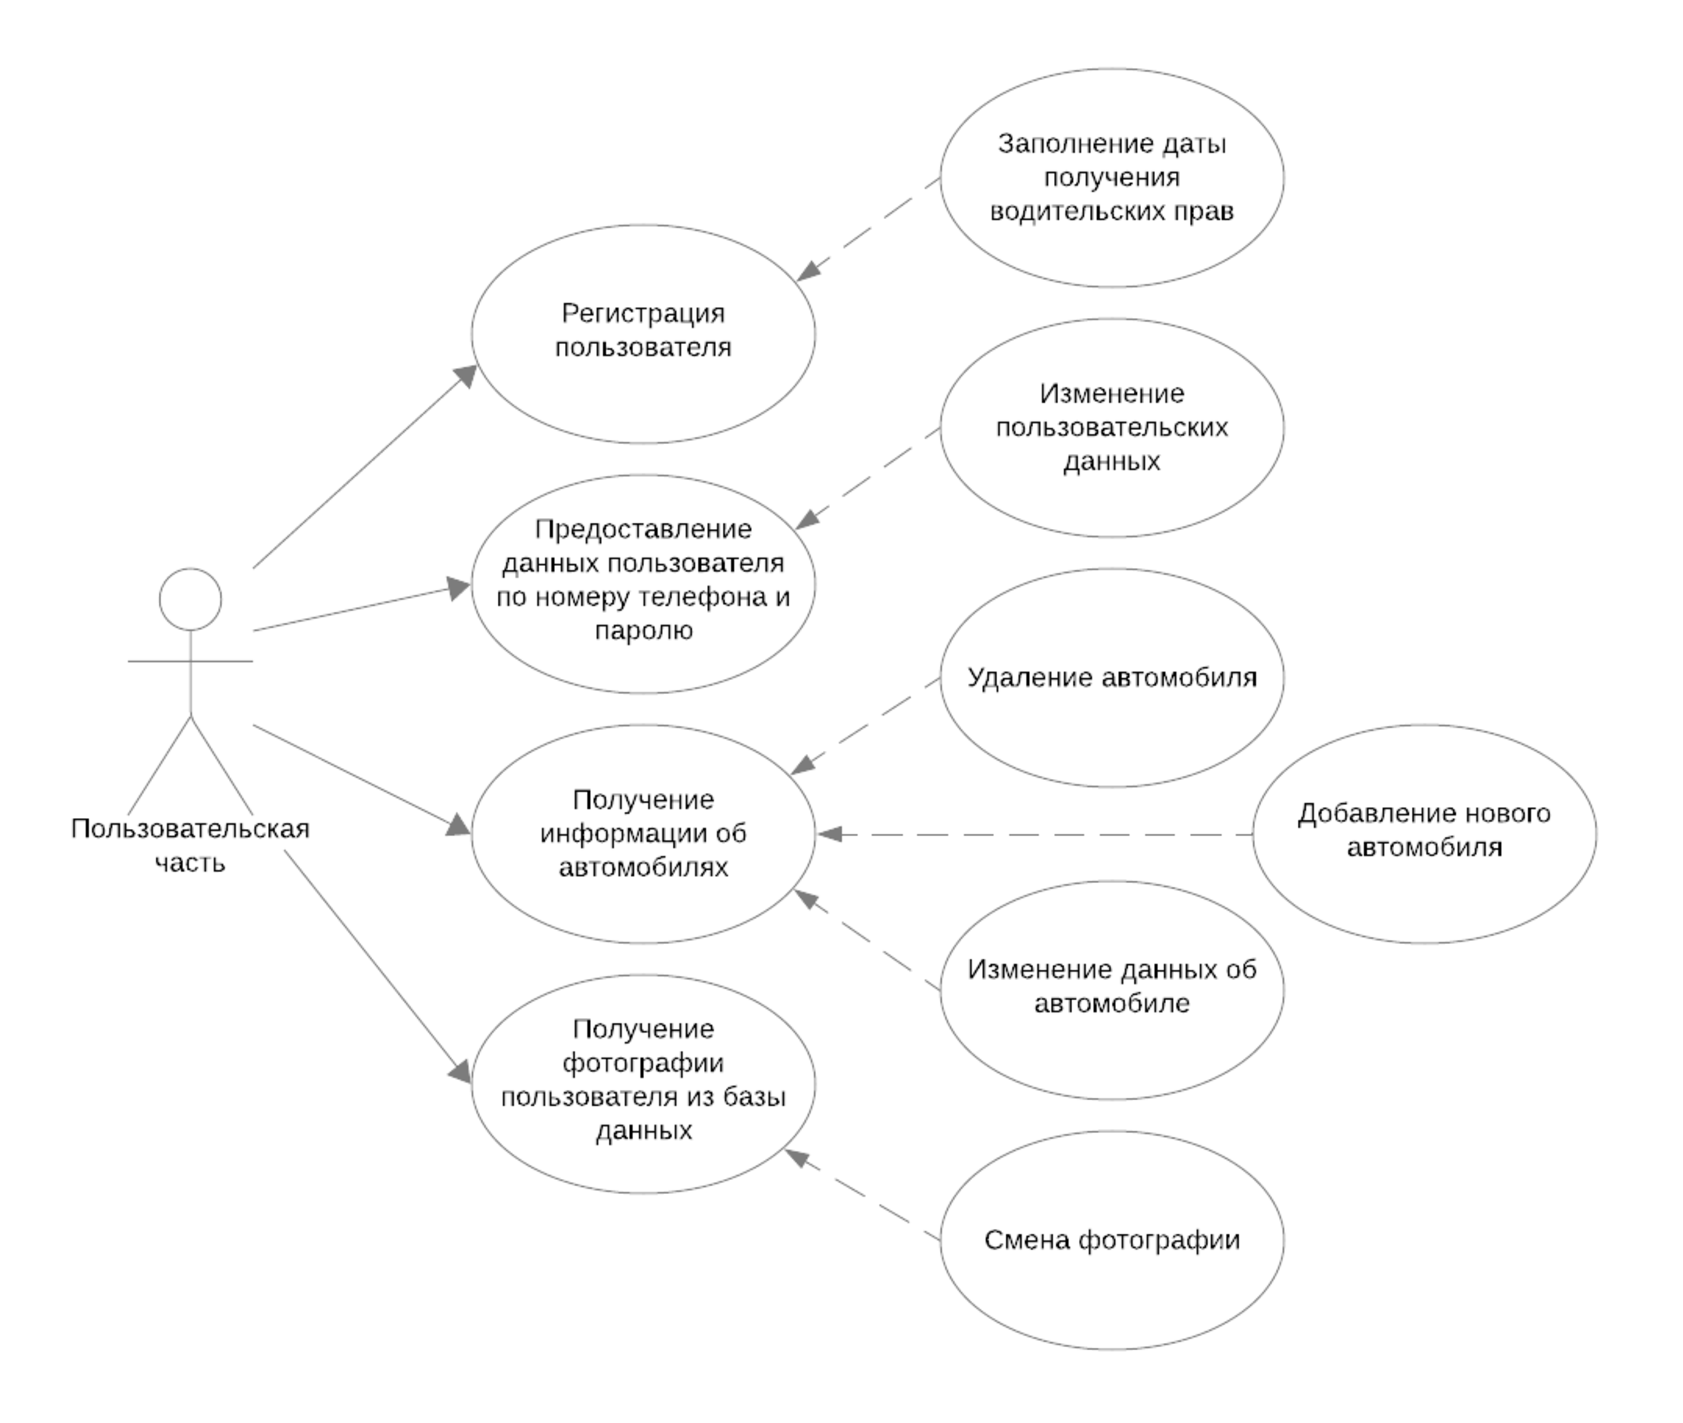
\includegraphics[width=0.7\linewidth]{images/Precedent1}
	\caption{Диаграмма вариантов использования, часть 1}
	\label{fig:precedent1}
\end{figure}

\begin{figure}[H]
	\centering
	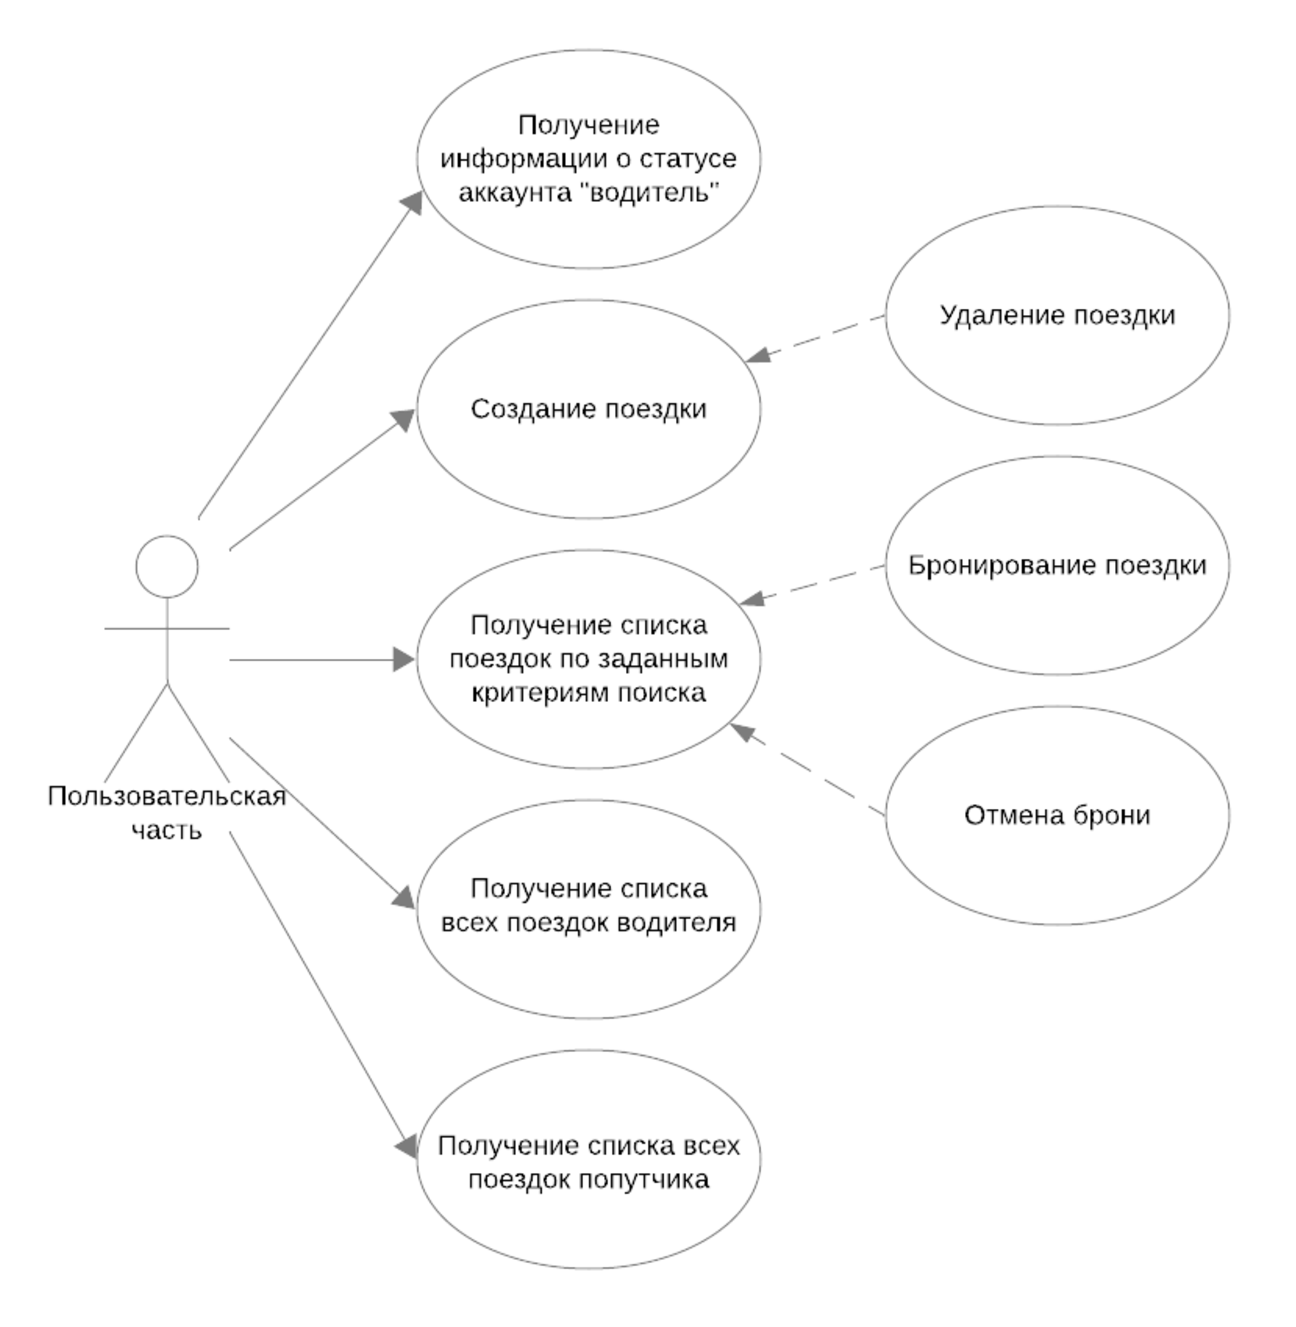
\includegraphics[width=0.7\linewidth]{images/Precedent2}
	\caption{Диаграмма вариантов использования, чать 2}
	\label{fig:precedent2}
\end{figure}

\begin{figure}[H]
	\centering
	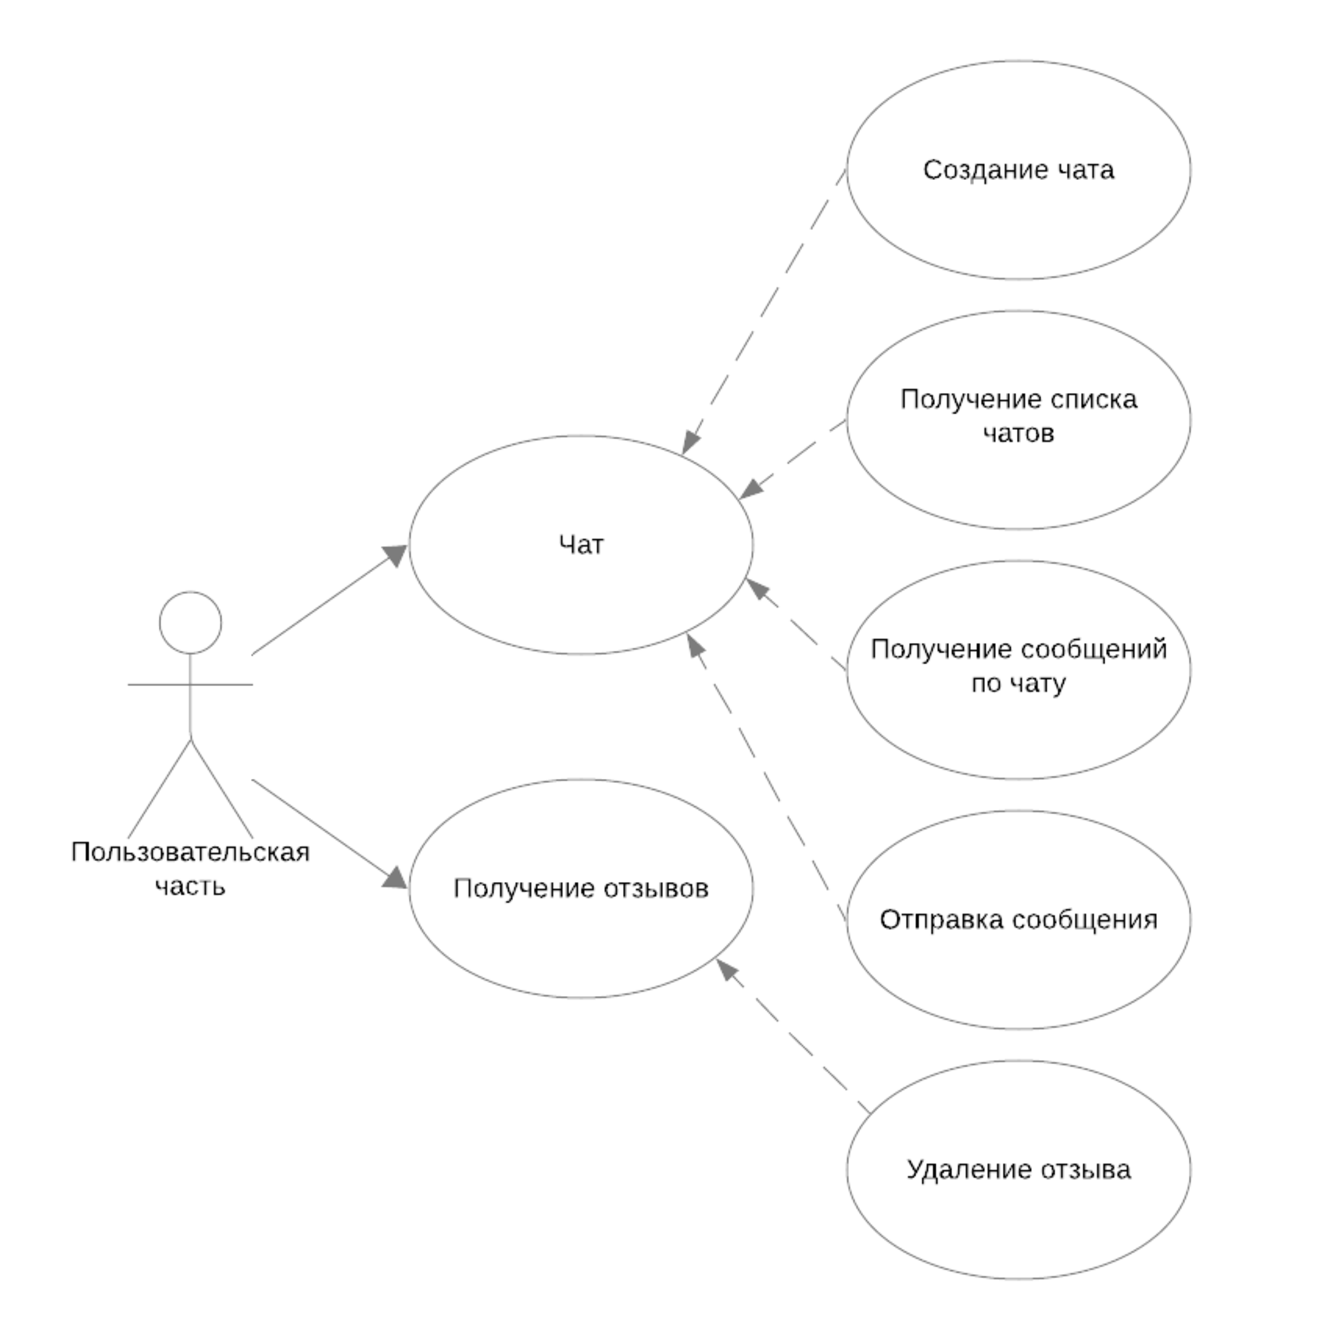
\includegraphics[width=0.7\linewidth]{images/Precedent3}
	\caption{Диаграмма вариантов использования, часть 3}
	\label{fig:precedent3}
\end{figure}

\paragraph{Вариант использования «Регистрация пользователя»}
Заинтересованные лица и их требования: пользователи программной системы, которые хотят зарегистрировать аккаунт, с целью получения возможности использовать функционал приложения для подбора попутчиков. Предусловие: на пользовательском устройстве открыто приложение AutoStop. Постусловие: пользователь регистрирует аккаунт как попутчик.
Основной успешный сценарий:

\begin{enumerate}
	\item Со стороны пользовательской части на сервер отправеляется URI запрос с пользовательскими данными в формате json файла.
	\item Сервер отслеживает запрос, проверяя возможность регистрации под переданным номером телефона.
	\item Сервер запускает скрипт на добавление пользователя в базу данных.
	\item Сервер отправляет на frontend статус OK.
\end{enumerate}

\paragraph{Вариант использования «Регистрация водителя»}
Заинтересованные лица и их требования: пользователи программной системы, которые хотят расширить возможности своей учетной записи, с целью создания поездок в используемом приложении. Предусловие: пользователь уже осуществил базовую регистрацию аккаунта. Постусловие: пользователь регистрирует аккаунт как водитель.
Основной успешный сценарий:

\begin{enumerate}
	\item Со стороны пользовательской части на сервер отправеляется URI запрос с номером телефона пользователя и датой получения водительского удостоверения.
	\item Сервер отслеживает запрос, и дополняет информацию по аккаунту пользователя.
	\item Сервер отправляет на frontend статус OK.
\end{enumerate}

\paragraph{Вариант использования «Авторизация»}
Заинтересованные лица и их требования: пользователи программной системы, которые хотят войти в систему подбора попутчиков для автомобильных поездок под своей учетной записью. Предусловие: пользователь прошел регистрацию и имеет аккаунт. Постусловие: пользователь входит в систему.
Основной успешный сценарий:

\begin{enumerate}
	\item Со стороны пользовательской части на сервер отправеляется URI запрос с номером телефона пользователя и паролем в формате json файла.
	\item Сервер отслеживает запрос, и находит пользователя по переданным данным.
	\item Сервер отправляет на frontend json файл с пользовательскими данными.
\end{enumerate}

\paragraph{Вариант использования «Изменение пользовательских данных»}
Заинтересованные лица и их требования: пользователи программной системы, которые хотят изменить личные данные в системе подбора попутчиков для автомобильных поездок. Предусловие: пользователь осуществил вход под своей учетной записью. Постусловие: пользователь изменяет данные аккаунта.
Основной успешный сценарий:

\begin{enumerate}
	\item Со стороны пользовательской части на сервер отправеляется URI запрос с номером телефона пользователя и измененными данными в формате json файла.
	\item Сервер отслеживает запрос, и находит пользователя по переданным данным.
	\item Сервер запускает скрипт на изменение в БД.
	\item Сервер отправляет на frontend статус OK.
\end{enumerate}

\paragraph{Вариант использования «Получение информации об автомобилях»}
Заинтересованные лица и их требования: пользователи программной системы, которые хотят получить список всех автомобилей, доступных под используемым профилем. Предусловие: пользователь осуществил вход под своей учетной записью и является водителем в системе. Постусловие: пользователь получает список машин.
Основной успешный сценарий:

\begin{enumerate}
	\item Со стороны пользовательской части на сервер отправеляется URI запрос с номером телефона пользователя.
	\item Сервер отслеживает запрос, и находит все автомобили зарегистрированные на данного пользователя.
	\item Сервер отправляет на frontend список всех найденых машин.
\end{enumerate}

\paragraph{Вариант использования «Добавление нового автомобиля»}
Заинтересованные лица и их требования: пользователи программной системы, которые хотят добавить автомобиль, для дальнейшего использования в поездках. Предусловие: пользователь осуществил вход под своей учетной записью и является водителем в системе. Постусловие: пользователь добавляет автомобиль в свой профиль.
Основной успешный сценарий:

\begin{enumerate}
	\item Со стороны пользовательской части на сервер отправеляется URI запрос с номером телефона пользователя и данными об автомобиле в формате json файла.
	\item Сервер отслеживает запрос, и добавляет сведения об автомобиле указанному пользователю.
	\item Сервер отправляет на frontend сообщение со статусом OK.
\end{enumerate}

\paragraph{Вариант использования «Изменение данных об автомобиле»}
Заинтересованные лица и их требования: пользователи программной системы, которые изменить указанные данные о машине в профиле. Предусловие: пользователь осуществил вход под своей учетной записью и является водителем в системе. У пользователя есть хотя бы 1 автомобиль в профиле. Постусловие: пользователь изменяеь данные о машине.
Основной успешный сценарий:

\begin{enumerate}
	\item Со стороны пользовательской части на сервер отправеляется URI запрос с ГРЗ автомобиля и обновленными данными в формате json файла.
	\item Сервер отслеживает запрос, и обновляет данные, на новые.
	\item Сервер отправляет на frontend сообщение со статусом OK.
\end{enumerate}

\paragraph{Вариант использования «Удаление автомобиля»}
Заинтересованные лица и их требования: пользователи программной системы, которые хотят удалить существующий автомобиль из профиля. Предусловие: пользователь осуществил вход под своей учетной записью и является водителем в системе. У пользователя есть хотя бы 1 автомобиль в профиле. Постусловие: пользователь удаляет данные о машине.
Основной успешный сценарий:

\begin{enumerate}
	\item Со стороны пользовательской части на сервер отправеляется URI запрос с ГРЗ автомобиля который необходимо удалить.
	\item Сервер отслеживает запрос, и находит указанную машину.
	\item Сервер запускает скрипт на удаление автомобиля из БД.
	\item Сервер отправляет на frontend сообщение со статусом OK.
\end{enumerate}

\paragraph{Вариант использования «Получение фото профиля»}
Заинтересованные лица и их требования: пользователи программной системы, которые осуществляют вход под своей учетной записью. Предусловие: пользователь прошел базовую регистрацию и имеет аккаунт в системе. Постусловие: пользователь получает фотографию своего профиля.
Основной успешный сценарий:

\begin{enumerate}
	\item Со стороны пользовательской части на сервер отправеляется URI запрос с номером телефона пользователя.
	\item Сервер отслеживает запрос, и находит фото профиля в базе данных.
	\item Сервер отправляет на frontend изображение.
\end{enumerate}

\paragraph{Вариант использования «Смена фото профиля»}
Заинтересованные лица и их требования: пользователи программной системы, которые хотят заменить фотографию профиля на новую. Предусловие: пользователь прошел базовую регистрацию и имеет аккаунт в системе. Постусловие: пользователь изменяет фотографию своего профиля.
Основной успешный сценарий:

\begin{enumerate}
	\item Со стороны пользовательской части на сервер отправеляется URI запрос с номером телефона пользователя и фографией в формате json файла.
	\item Сервер отслеживает запрос, и находит пользователя с указанным номером телефона.
	\item Сервер запускает скрипт на изменение фотографии в БД.
	\item Сервер отправляет на frontend сообщение со статусом OK.
\end{enumerate}

\paragraph{Вариант использования «Получение информации о статусе аккаунта}
Заинтересованные лица и их требования: пользователи программной системы, которые хотят создать новую поездку в системе. Предусловие:  пользователь вошел под своим аккунтом в приложение. Постусловие: пользователь получает возможность создать поездку в системе.
Основной успешный сценарий:

\begin{enumerate}
	\item Со стороны пользовательской части на сервер отправеляется URI запрос с номером телефона пользователя.
	\item Сервер отслеживает запрос, и находит запись с датой получения водительского удостоверения.
	\item Сервер отправляет на frontend json файл с датой получения прав.
\end{enumerate}

\paragraph{Вариант использования «Создание поездки»}
Заинтересованные лица и их требования: пользователи программной системы, которые хотят создать новую поездку в системе. Предусловие:  пользователь вошел под своим аккунтом в приложение и прошел проверку на наличие водительского удостоверения. Постусловие: пользователь создает поезку в системе для подбора попутчиков.
Основной успешный сценарий:

\begin{enumerate}
	\item Со стороны пользовательской части на сервер отправеляется URI запрос с данными о поездке, которую необходимо создать, в формате json файла.
	\item Сервер отслеживает запрос, и добавляет данные о поездке в БД.
	\item Сервер отправляет на frontend сообщение со статусом  OK.
\end{enumerate}

\paragraph{Вариант использования «Удаление поездки»}
Заинтересованные лица и их требования: пользователи программной системы, у которых есть необходимость у далении существующей поездки. Предусловие:  пользователь вошел под своим аккунтом в приложение. В системе есть хотя бы одна поездка созданная до данным профилем. Постусловие: пользователь удаляет поезку в системе для подбора попутчиков.
Основной успешный сценарий:

\begin{enumerate}
	\item Со стороны пользовательской части на сервер отправеляется URI запрос уникальным идентификатором удаляемой поездки.
	\item Сервер отслеживает запрос, и удаляет поездку из системы.
	\item Сервер отправляет на frontend сообщение со статусом  OK.
\end{enumerate}

\paragraph{Вариант использования «Получение списка поездок по заданным критериям поиска»}
Заинтересованные лица и их требования: пользователи программной системы, у которых есть необходимость в поиске подходящей поездки. Предусловие:  пользователь вошел под своим аккунтом в приложение. Постусловие: попутчик получает список поездок по заданным условиям поиска.
Основной успешный сценарий:

\begin{enumerate}
	\item Со стороны пользовательской части на сервер отправеляется URI запрос с данными, на основе которых необходимо осуществить выборку из существующих поездок в системе.
	\item Сервер отслеживает запрос, и находит все поездки, удовлетворящие условиям поиска.
	\item Сервер отправляет на frontend список всех найденых поездок в формате json файла.
\end{enumerate}

\paragraph{Вариант использования «Бронирование поездки»}
Заинтересованные лица и их требования: пользователи программной системы, целью которых является бронирование поездки в системе для подбора попутчиков. Предусловие:  пользователь вошел под своим аккунтом в приложение. В системе имеются активные поездки. Постусловие: попутчик бронирует поездку.
Основной успешный сценарий:

\begin{enumerate}
	\item Со стороны пользовательской части на сервер отправеляется URI запрос с пользовательскими данные и информацией о бронируемой поездке.
	\item Сервер отслеживает запрос, и записывает пользователя в поездку.
	\item Сервер отправляет на frontend ответ со статусом OK.
\end{enumerate}

\paragraph{Вариант использования «Отмена брони»}
Заинтересованные лица и их требования: пользователи программной системы, которые хотят отменить бронирование поездки. Предусловие:  пользователь вошел под своим аккунтом в приложение. У пользователя есть бронь. Постусловие: попутчик отменяет бронь.
Основной успешный сценарий:

\begin{enumerate}
	\item Со стороны пользовательской части на сервер отправеляется URI запрос с пользовательскими данные и информацией о бронируемой поездке.
	\item Сервер отслеживает запрос, и удаляет из базы данных информацию о брони.
	\item Сервер отправляет на frontend ответ со статусом OK.
\end{enumerate}

\paragraph{Вариант использования «Получения списка всех поездок для водителя»}
Заинтересованные лица и их требования: пользователи программной системы, получить список всех созданных поездок данным водителем. Предусловие:  пользователь вошел под своим аккунтом в приложение. У пользователя есть хотя бы одна созданная поездка. Постусловие: водитель получает список всех созданных поездок.
Основной успешный сценарий:

\begin{enumerate}
	\item Со стороны пользовательской части на сервер отправеляется URI запрос с номером телефона водителя.
	\item Сервер отслеживает запрос, и находит пользовательские поездки.
	\item Сервер отправляет на frontend список всех созданных поездок со статусом "<водитель"> в формате json файла.
\end{enumerate}

\paragraph{Вариант использования «Получения списка всех поездок для водителя»}
Заинтересованные лица и их требования: пользователи программной системы, получить список всех созданных поездок данным водителем. Предусловие:  пользователь вошел под своим аккунтом в приложение. У пользователя есть хотя бы одна созданная поездка. Постусловие: водитель получает список всех созданных поездок.
Основной успешный сценарий:

\begin{enumerate}
	\item Со стороны пользовательской части на сервер отправеляется URI запрос с номером телефона водителя.
	\item Сервер отслеживает запрос, и находит пользовательские поездки.
	\item Сервер отправляет на frontend список всех созданных поездок со статусом "<водитель"> в формате json файла.
\end{enumerate}

\paragraph{Вариант использования «Получения списка всех поездок для попутчика»}
Заинтересованные лица и их требования: пользователи программной системы, получить список всех забронированных поездок. Предусловие:  пользователь вошел под своим аккунтом в приложение. У пользователя есть хотя бы одна забронированная поездка. Постусловие: попутчик получает список всех созданных поездок.
Основной успешный сценарий:

\begin{enumerate}
	\item Со стороны пользовательской части на сервер отправеляется URI запрос с номером телефона попутчика.
	\item Сервер отслеживает запрос, и находит пользовательские поездки.
	\item Сервер отправляет на frontend список всех забронированных поездок в формате json файла.
\end{enumerate}

\paragraph{Вариант использования «Создание чата»}
Заинтересованные лица и их требования: пользователи программной системы, которые хотят свзяаться с водителем для обсуждения планов поездки. Предусловие:  пользователь вошел под своим аккунтом в приложение и осуществил поиск поездок. Постусловие: попутчик создает чат с водителем.
Основной успешный сценарий:

\begin{enumerate}
	\item Со стороны пользовательской части на сервер отправеляется URI запрос с номеромами телефона попутчика и водителя.
	\item Сервер отслеживает запрос, и проверяет наличие чата.
	\item Сервер создает новый чат.
	\item Сервер отправляет на frontend информацию о новом созданном чате в формате json файла.
\end{enumerate}

\paragraph{Вариант использования «Получение списка чатов»}
Заинтересованные лица и их требования: пользователи программной системы, которые хотят получить полную информацю по имеющимся чатам. Предусловие:  пользователь вошел под своим аккунтом в приложение и имеет хотя бы 1 чат. Постусловие: пользователь получает полный список чатов.
Основной успешный сценарий:

\begin{enumerate}
	\item Со стороны пользовательской части на сервер отправеляется URI запрос с номеромами телефона пользователя.
	\item Сервер отслеживает запрос, и находит информацю по чатам.
	\item Сервер отправляет на frontend список всех чатов в формате json файла.
\end{enumerate}

\paragraph{Вариант использования «Получение сообщений по чату»}
Заинтересованные лица и их требования: пользователи программной системы, которые хотят получить все сообщения по выбранному чату. Предусловие:  пользователь вошел под своим аккунтом в приложение и имеет хотя бы 1 чат с сообщениями. Постусловие: пользователь получает полный список сообщений.
Основной успешный сценарий:

\begin{enumerate}
	\item Со стороны пользовательской части на сервер отправеляется URI запрос с уникальным идентификатором чата.
	\item Сервер отслеживает запрос, и находит сообщения по указанному чату.
	\item Сервер отправляет на frontend список всех сообщений в формате json файла.
\end{enumerate}

\paragraph{Вариант использования «Отправка сообщения»}
Заинтересованные лица и их требования: пользователи программной системы, которые хотят установисть связь с собеседником через отправку сообщений. Предусловие:  пользователь вошел под своим аккунтом в приложение и имеет хотя бы 1 чат. Постусловие: пользователь отправляет сообщение собеседнику.
Основной успешный сценарий:

\begin{enumerate}
	\item Со стороны пользовательской части на сервер отправеляется URI запрос с уникальным идентификатором чата и текстом сообщения в формате json файла.
	\item Сервер отслеживает запрос, и добавляет сообщение в БД.
	\item Сервер отправляет на frontend ответ со статусом OK.
\end{enumerate}

\paragraph{Вариант использования «Получение отзывов»}
Заинтересованные лица и их требования: пользователи программной системы, которые хотят просмотреть список всех отзывов по профилю. Предусловие:  пользователь имеет хотя бы 1 отзыв. Постусловие: пользователь получает список всех отзывов.
Основной успешный сценарий:

\begin{enumerate}
	\item Со стороны пользовательской части на сервер отправеляется URI запрос с номером телефона пользователя.
	\item Сервер отслеживает запрос, и производит поик всех отзывов.
	\item Сервер отправляет на frontend список всех отзывов.
\end{enumerate}

\paragraph{Вариант использования «Удаление отзыва»}
Заинтересованные лица и их требования: пользователи программной системы, которые хотят удалить оставленный отзыв. Предусловие:  пользователь имеет хотя бы 1 отзыв. Постусловие: пользователь удаляет свой отзывов.
Основной успешный сценарий:

\begin{enumerate}
	\item Со стороны пользовательской части на сервер отправеляется URI запрос с уникальным идентификатором отзыва.
	\item Сервер отслеживает запрос, и производит удаление отзыва.
	\item Сервер отправляет на frontend ответ со статусом OK.
\end{enumerate}

\subsubsection{Нефункциональные требования к программной системе}
\paragraph{Требования к надежности}

В процессе работы серверной части программной системы могут произойти следующие аварийные ситуации:

\begin{itemize}
\item Потеря доступа к сети Интернет. Возможные причины включают проблемы с сетью, сбои маршрутизаторов или изменения в конфигурации сети.
\item Аварийное отключение электропитания. Это может произойти из-за технических проблем в дата-центре, аварий на электросетях или природных катаклизмов.
\item Сбой операционной системы сервера. Операционная система может выйти из строя по причине аппаратных или программных сбоев, ошибок обновлений или атак вредоносного ПО.
\end{itemize}

Для минимизации вероятности возникновения аварийных событий серверные компоненты программной системы должны быть размещены на выделенных серверах в дата-центрах хостинг-провайдеров. Операционная система должна получать регулярные накопительные обновления.

\paragraph{Требования к безопасности}
Для защиты системы от несанкционированного доступа каждый запрос к базе данных должен проходить через специальный набор правил. Пользователь, не имеющий доступа к определенным данным должен не
иметь возможности взаимодействовать с ними.

Для доступа к приложению пользователю необходимо пройти авторизацию в системе.

Для возможности авторизации в системе, пользователь должен пройти регистрацию.

Фунции доступные водительскому акаунту не должны быть доступны для попутчика.

\paragraph{Требования к программному обеспечению}

Для реализации серверной части программной системы должен быть использован язык высокого уровня C\#.

В качестве системы управления базой данных (СУБД) должна быть использована система Microsoft SQL Server, разработанная компанией Microsoft.

Для реализации модуля чатов и сообщений необходим асинхронный подход, для ускорения работы системы и оптимизации используемых ресурсов сервера.

За обеспечение целостности данных должнен отвечать автоматический сервис, который запускается на сервере каждые 10 минут. С целью добавления неактуальных поездок в архив. Это снизит нагрузку при поиске данных, связанных с пользовательскими поездками.

\paragraph{Требования к аппаратному обеспечению}

Для обеспечения стабильной и эффективной работы написанной программной реализации, сервер должен соответствовать следующим требованиям к аппаратному обеспечению:

Процессор (CPU)
\begin{itemize}
	\item Тип: Многоядерный процессор с поддержкой технологии многопоточности.
	\item Рекомендуемые модели: Intel Xeon серии E5 или выше, AMD EPYC или Ryzen 7 и выше.
	\item Частота: Минимум 2.4 ГГц на ядро.
	\item Количество ядер: Минимум 4 физических ядра.
\end{itemize}

Оперативная память (RAM)
\begin{itemize}
	\item Объем: Минимум 16 ГБ, рекомендуется 32 ГБ и выше в зависимости от нагрузки и количества одновременно работающих приложений.
	\item Тип: DDR4 с частотой не ниже 2400 МГц.
\end{itemize}

Накопитель (SSD/HDD)
\begin{itemize}
	\item Тип: SSD для основной системы и данных, HDD можно использовать для хранения архивов и резервных копий.
	\item Объем: Минимум 500 ГБ для SSD, рекомендуется 1 ТБ и более.
	\item Скорость чтения/записи: Не менее 500 МБ/с для SSD.
\end{itemize}

Сетевое оборудование
\begin{itemize}
	\item Сетевая карта: Гигабитная Ethernet-карта (1 Gbps).
	\item Дополнительно: Поддержка резервирования сетевых подключений для обеспечения отказоустойчивости.
\end{itemize}

Источник бесперебойного питания (ИБП)
\begin{itemize}
	\item Мощность: Достаточная для поддержания работы сервера в течение минимум 30 минут при отключении электропитания.
	\item Функции: Возможность автоматического корректного завершения работы сервера при длительном отключении питания.
\end{itemize}

Система охлаждения
\begin{itemize}
	\item Тип: Эффективная система охлаждения для поддержания стабильной температуры процессора и других компонентов.
	\item Дополнительно: Наличие нескольких вентиляторов и/или жидкостной системы охлаждения для серверов с высокими нагрузками.
\end{itemize}

Корпус и питание
\begin{itemize}
	\item Корпус: Серверный корпус форм-фактора Tower или Rack, обеспечивающий хорошую вентиляцию.
	\item Блок питания: Сертифицированный блок питания с мощностью не менее 750 Вт, с запасом мощности для дополнительного оборудования.
\end{itemize}

Дополнительные требования
\begin{itemize}
	\item Резервирование: Возможность установки резервных блоков питания и дисков для обеспечения отказоустойчивости.
	\item Мониторинг: Встроенные системы мониторинга состояния компонентов и температуры.
\end{itemize}

\subsection{Требования к оформлению документации}
Требования к стадиям разработки программ и программной документации для вычислительных машин, комплексов и систем независимо от их
назначения и области применения, этапам и содержанию работ устанавливаются ГОСТ 19.102–77.
Программная документация должна включать в себя:
\begin{itemize}
\item Анализ предметной области.
\item Техническое задание.
\item Технический проект.
\item Рабочий проект.
\end{itemize}
\section{Технический проект}
\subsection{Общая характеристика организации решения задачи}

Полное наименование системы: кроссплатформенная программная система подбора попутчиков для автомобильных поездок.

Разрабатываемая программная система представляет собой платформу, позволяющую пользователям находить попутчиков для созданных автомобильных поездок. Данная система построена на клиент-серверной архитектуре.

Сервер – backend-модуль[{21}][{11}][{31}], обрабатывающий запросы клиентов. Сервер в данной программной системе один.

Функции, выполняемые на стороне сервера:

\begin{itemize}
	\item хранение, защита и доступ к данным;
	\item обработка поступающих клиентских запросов;
	\item поддержание целостности и актуальности данных;
	\item формирование и отправка ответов клиентам.
\end{itemize}

Одним из основных компонентов системы является база данных. В ней хранится практически вся информация, необходимая для работы системы, от данных пользователей до информации о предлагаемых и запрашиваемых поездках, а так же сведения об автомобилях, мессенджер, отзывы и рейтинг.

Задачи разработки включают:

\begin{itemize}
	\item проектирование и создание базы данных;
	\item разработка фонового сервиса для поддержания актуальности данных о поездках;
	\item проектирование и создание моделей данных;
	\item разработку контроллеров для обработки запросов;
	\item реализацию функционала для взаимодействия с базой данных.
\end{itemize}

\subsection{Обоснование выбора технологий проектирования}

Используемые для создания программно-информационной системы
языки и технологии отвечают современным практикам разработки, позволяют достичь высокой производительности и отказоустойчивости программы.

\subsubsection{Язык программирования C\#}

C\#[{1}][{2}][{3}] является одним из наиболее популярных и мощных языков программирования, который был разработан корпорацией Microsoft в рамках платформы .NET[{5}][{6}][{7}][{8}]. Одним из основных преимуществ C\# является его современный синтаксис, который сочетает в себе простоту и выразительность, что делает его удобным для изучения и использования как начинающими, так и опытными программистами. Этот язык позволяет разработчикам писать чистый, понятный и поддерживаемый код, что особенно важно при создании крупных и сложных приложений.

Еще одной значимой чертой C\# является его поддержка объектно-ориентированного программирования (ООП){[22]}{[23]}{[24]}. Это позволяет разработчикам создавать приложения, основываясь на принципах инкапсуляции, наследования и полиморфизма, что способствует созданию гибких и масштабируемых программных решений. ООП также облегчает повторное использование кода, что снижает затраты на разработку и поддержку программного обеспечения.

Богатый набор библиотек и инструментов, доступных для C\#, существенно упрощает разработку программ. Эти библиотеки покрывают широкий спектр задач — от работы с базами данных и сетевыми взаимодействиями до создания пользовательских интерфейсов и работы с файлами. Благодаря этому разработчики могут сосредоточиться на решении бизнес-задач, не тратя много времени на создание базовой функциональности с нуля.

Среда разработки Visual Studio[{9}][{10}][{13}][{14}], в которой часто ведется разработка на C\#, предлагает мощные средства для написания, отладки и тестирования кода. Интегрированные средства автоматизации, рефакторинга и анализа кода помогают разработчикам повышать продуктивность и качество конечного продукта. Это позволяет быстро находить и исправлять ошибки, а также оптимизировать код для повышения его производительности.

C\# также обладает высокой безопасностью типов, что предотвращает многие распространенные ошибки, такие как доступ к неинициализированным переменным или некорректное приведение типов. Управление памятью в C\# осуществляется с помощью сборщика мусора, что упрощает процесс управления ресурсами и снижает вероятность утечек памяти.

Кроме того, сообщество разработчиков C\# активно и постоянно растет, предоставляя богатый выбор ресурсов для обучения и обмена опытом. Это включает в себя форумы, блоги, видеоуроки и другие формы поддержки, которые помогают разработчикам быстро находить ответы на возникающие вопросы и постоянно совершенствовать свои навыки.

Таким образом, выбор C\# в качестве языка программирования предоставляет разработчикам мощные инструменты для создания современных, эффективных и надежных приложений, что делает его отличным выбором для самых разнообразных проектов.

\subsubsection{Фреймворк ASP.net}

ASP.NET[{15}][{16}][{17}][{18}] — это мощная и гибкая платформа для разработки веб-приложений, созданная корпорацией Microsoft. Один из основных факторов, делающих ASP.NET привлекательным выбором для разработчиков, — это его интеграция с экосистемой .NET. Это позволяет использовать все возможности языка программирования C\#, а также широкий набор библиотек и инструментов, что существенно ускоряет процесс разработки и упрощает создание высокопроизводительных и масштабируемых веб-приложений.

ASP.NET предоставляет разработчикам множество возможностей для создания динамических веб-страниц и приложений. Он поддерживает модель программирования, которая включает в себя серверные элементы управления, такие как формы и сетки данных, что позволяет создавать интерактивные и отзывчивые пользовательские интерфейсы с минимальными усилиями. Это особенно важно для создания сложных веб-приложений, которые требуют высокого уровня интерактивности и пользовательского опыта.

Одним из ключевых преимуществ ASP.NET является его высокая производительность. Платформа оптимизирована для обработки больших объемов запросов и может эффективно управлять ресурсами, что позволяет создавать быстрые и отзывчивые веб-приложения. ASP.NET также поддерживает асинхронное программирование, что улучшает масштабируемость приложений и снижает нагрузку на серверы.

Безопасность является еще одной важной чертой ASP.NET. Платформа предоставляет встроенные механизмы защиты от распространенных угроз веб-безопасности, таких как межсайтовый скриптинг (XSS)[{19}][{20}], SQL-инъекции[{25}][{26}]и другие виды атак. Это позволяет разработчикам сосредоточиться на функциональности приложений, не беспокоясь о внедрении сложных мер безопасности.

ASP.NET также поддерживает модульность и повторное использование кода. Это достигается благодаря компонентам, таким как контроллеры и представления в ASP.NET MVC[{27}][{28}][{29}][{32}], которые могут быть легко переработаны и использованы в различных частях приложения. Это способствует более эффективной разработке и снижает затраты на поддержку кода.

Кроме того, сообщество разработчиков ASP.NET активно и постоянно растет. Это обеспечивает обширную базу знаний и ресурсов, доступных для обучения и обмена опытом. Форумы, блоги, документация и видеоуроки помогают разработчикам быстро находить решения для возникающих проблем и улучшать свои навыки.

Таким образом, выбор ASP.NET в качестве платформы для разработки веб-приложений предоставляет разработчикам мощные инструменты и возможности для создания надежных, безопасных и высокопроизводительных веб-приложений. Платформа сочетает в себе современные технологии и подходы, что делает её отличным выбором для самых разнообразных проектов, от небольших сайтов до крупных корпоративных приложений.

\subsubsection{Расширение T-SQL}

T-SQL (Transact-SQL) — это расширение стандартного языка SQL (Structured Query Language), разработанное корпорацией Microsoft для управления и манипулирования данными в реляционных базах данных, таких как Microsoft SQL Server. Одной из ключевых причин выбора T-SQL{[30]}{[33]} является его тесная интеграция с Microsoft SQL Server{[34]}{[35]}, что делает его мощным инструментом для разработки сложных запросов, процедур и скриптов, необходимых для управления данными и обеспечения их целостности.

Одним из значимых преимуществ T-SQL является его расширенные возможности по сравнению с обычным SQL. T-SQL включает в себя дополнительные конструкции, такие как циклы, условные операторы и встроенные функции, что позволяет разработчикам создавать более сложные и функциональные запросы. Это особенно важно для выполнения сложных бизнес-логик и операций с данными, которые требуют более гибких и мощных инструментов.

T-SQL также поддерживает создание хранимых процедур, триггеров и пользовательских функций. Хранимые процедуры позволяют выполнять сложные операции над данными, объединяя несколько SQL-запросов в один логический блок, что упрощает управление кодом и повышает его повторное использование. Триггеры позволяют автоматически выполнять определенные действия при изменении данных в таблице, что помогает поддерживать целостность данных и автоматизировать рутинные задачи.

Еще одной важной чертой T-SQL является его мощные средства для обработки и анализа данных. T-SQL предоставляет широкий набор функций для работы с текстом, датами, числами и другими типами данных, что облегчает выполнение различных операций над данными. Кроме того, T-SQL поддерживает создание временных таблиц и курсоров, что позволяет разработчикам эффективно управлять временными данными и выполнять сложные операции над ними.

Производительность также является важным аспектом T-SQL. Разработчики могут оптимизировать запросы с помощью индексов, оптимизатора запросов и других инструментов, что позволяет значительно повысить скорость выполнения операций над данными. Это особенно важно для работы с большими объемами данных, где производительность имеет критическое значение.

T-SQL также обеспечивает высокую степень безопасности данных. Разработчики могут использовать механизмы управления правами доступа, чтобы контролировать, кто и какие операции может выполнять над данными. Это помогает защитить данные от несанкционированного доступа и обеспечивать их конфиденциальность и целостность.

Кроме того, сообщество разработчиков T-SQL активно и постоянно растет, что обеспечивает широкий доступ к ресурсам для обучения и обмена опытом. Форумы, блоги, документация и видеоуроки помогают разработчикам быстро находить ответы на возникающие вопросы и совершенствовать свои навыки.

Таким образом, выбор T-SQL в качестве языка для работы с базами данных предоставляет разработчикам мощные и гибкие инструменты для управления данными, выполнения сложных операций и обеспечения их целостности и безопасности. Это делает T-SQL отличным выбором для разработки и поддержки надежных и эффективных решений для управления данными в корпоративных и других приложениях.

\subsubsection{Протокол связи HTTP}

HTTP (Hypertext Transfer Protocol) — это основополагающий протокол для передачи данных в интернете, который служит базой для обмена информацией между веб-серверами и клиентами, такими как браузеры. Протокол был разработан в начале 1990-х годов в Европейской организации по ядерным исследованиям (CERN) под руководством Тима Бернерса-Ли и Роберта Кайо, и с тех пор HTTP{[36]}{[37]} стал стандартом для передачи гипертекстовых документов в сети.

Одним из ключевых аспектов HTTP является его простота и универсальность. HTTP использует текстовый формат для передачи данных, что делает его легко читаемым и понятным как для машин, так и для людей. Запросы и ответы в HTTP формируются в виде строк, что упрощает процесс их анализа и отладки. Клиент (обычно браузер) отправляет запрос серверу, который обрабатывает его и возвращает ответ, содержащий запрашиваемые данные, статус выполнения запроса и метаинформацию.

HTTP — это протокол уровня приложения, который работает поверх других протоколов, таких как TCP/IP{[38]}{[39]}. Это позволяет ему обеспечивать надежную и последовательную доставку данных, а также корректировать ошибки передачи. HTTP поддерживает широкий спектр методов, каждый из которых предназначен для выполнения определенных действий. Наиболее распространенные из них — GET, POST, PUT и DELETE. Метод GET используется для запроса данных с сервера, POST — для отправки данных на сервер, PUT — для обновления существующих данных, а DELETE — для удаления данных.

Преимущество HTTP в его гибкости и способности адаптироваться под различные нужды. Например, современные веб-приложения используют HTTP для взаимодействия с API, что позволяет обмениваться данными между различными системами и сервисами. HTTP также поддерживает работу с мультимедийным контентом, таким как изображения, видео и аудио, что делает его идеальным для создания разнообразных веб-приложений.

Безопасность передачи данных является важным аспектом HTTP. Для обеспечения конфиденциальности и целостности данных используется протокол HTTPS, который представляет собой HTTP, работающий поверх SSL/TLS. HTTPS обеспечивает шифрование данных, передаваемых между клиентом и сервером, что защищает их от перехвата и изменения злоумышленниками. В наши дни использование HTTPS стало стандартом для большинства веб-сайтов, особенно тех, которые обрабатывают конфиденциальную информацию, такую как личные данные или данные кредитных карт.

Кроме того, HTTP поддерживает кэширование, что позволяет сохранять копии веб-страниц и других ресурсов для ускорения их загрузки при повторных обращениях. Это существенно улучшает пользовательский опыт, так как сокращает время ожидания и уменьшает нагрузку на серверы. Также HTTP поддерживает возможность сжатия данных, что снижает объем передаваемых данных и ускоряет их доставку.

HTTP продолжает развиваться, предлагая новые возможности и улучшения, которые позволяют разрабатывать более эффективные, безопасные и производительные веб-приложения. Независимо от сложности и масштабов проекта, HTTP остается фундаментальным инструментом для передачи данных в интернете.

\subsection{Проект данных программной системы}

На основании анализа предметной области из технического задания была разработана база данных.

База данных включает в себя следующие таблицы:

\begin{enumerate}
	\item Users - пользователи системы.
	\item Cars - пользовательские автомобили.
	\item Passengers - пассажиры забронировавшие поездку.
	\item Travels - поездки созданные водителем.
	\item DriverTravel - таблица связи, необходимая для привязки водителя и поездки.
	\item Chats - пользовательские чаты.
	\item Messages - сообщения в чате.
	\item Comments - комментарии под профилем.
\end{enumerate}

На рисунке 3.1 изображена ER-диаграмма базы данных.

\begin{figure}[H]
	\centering
	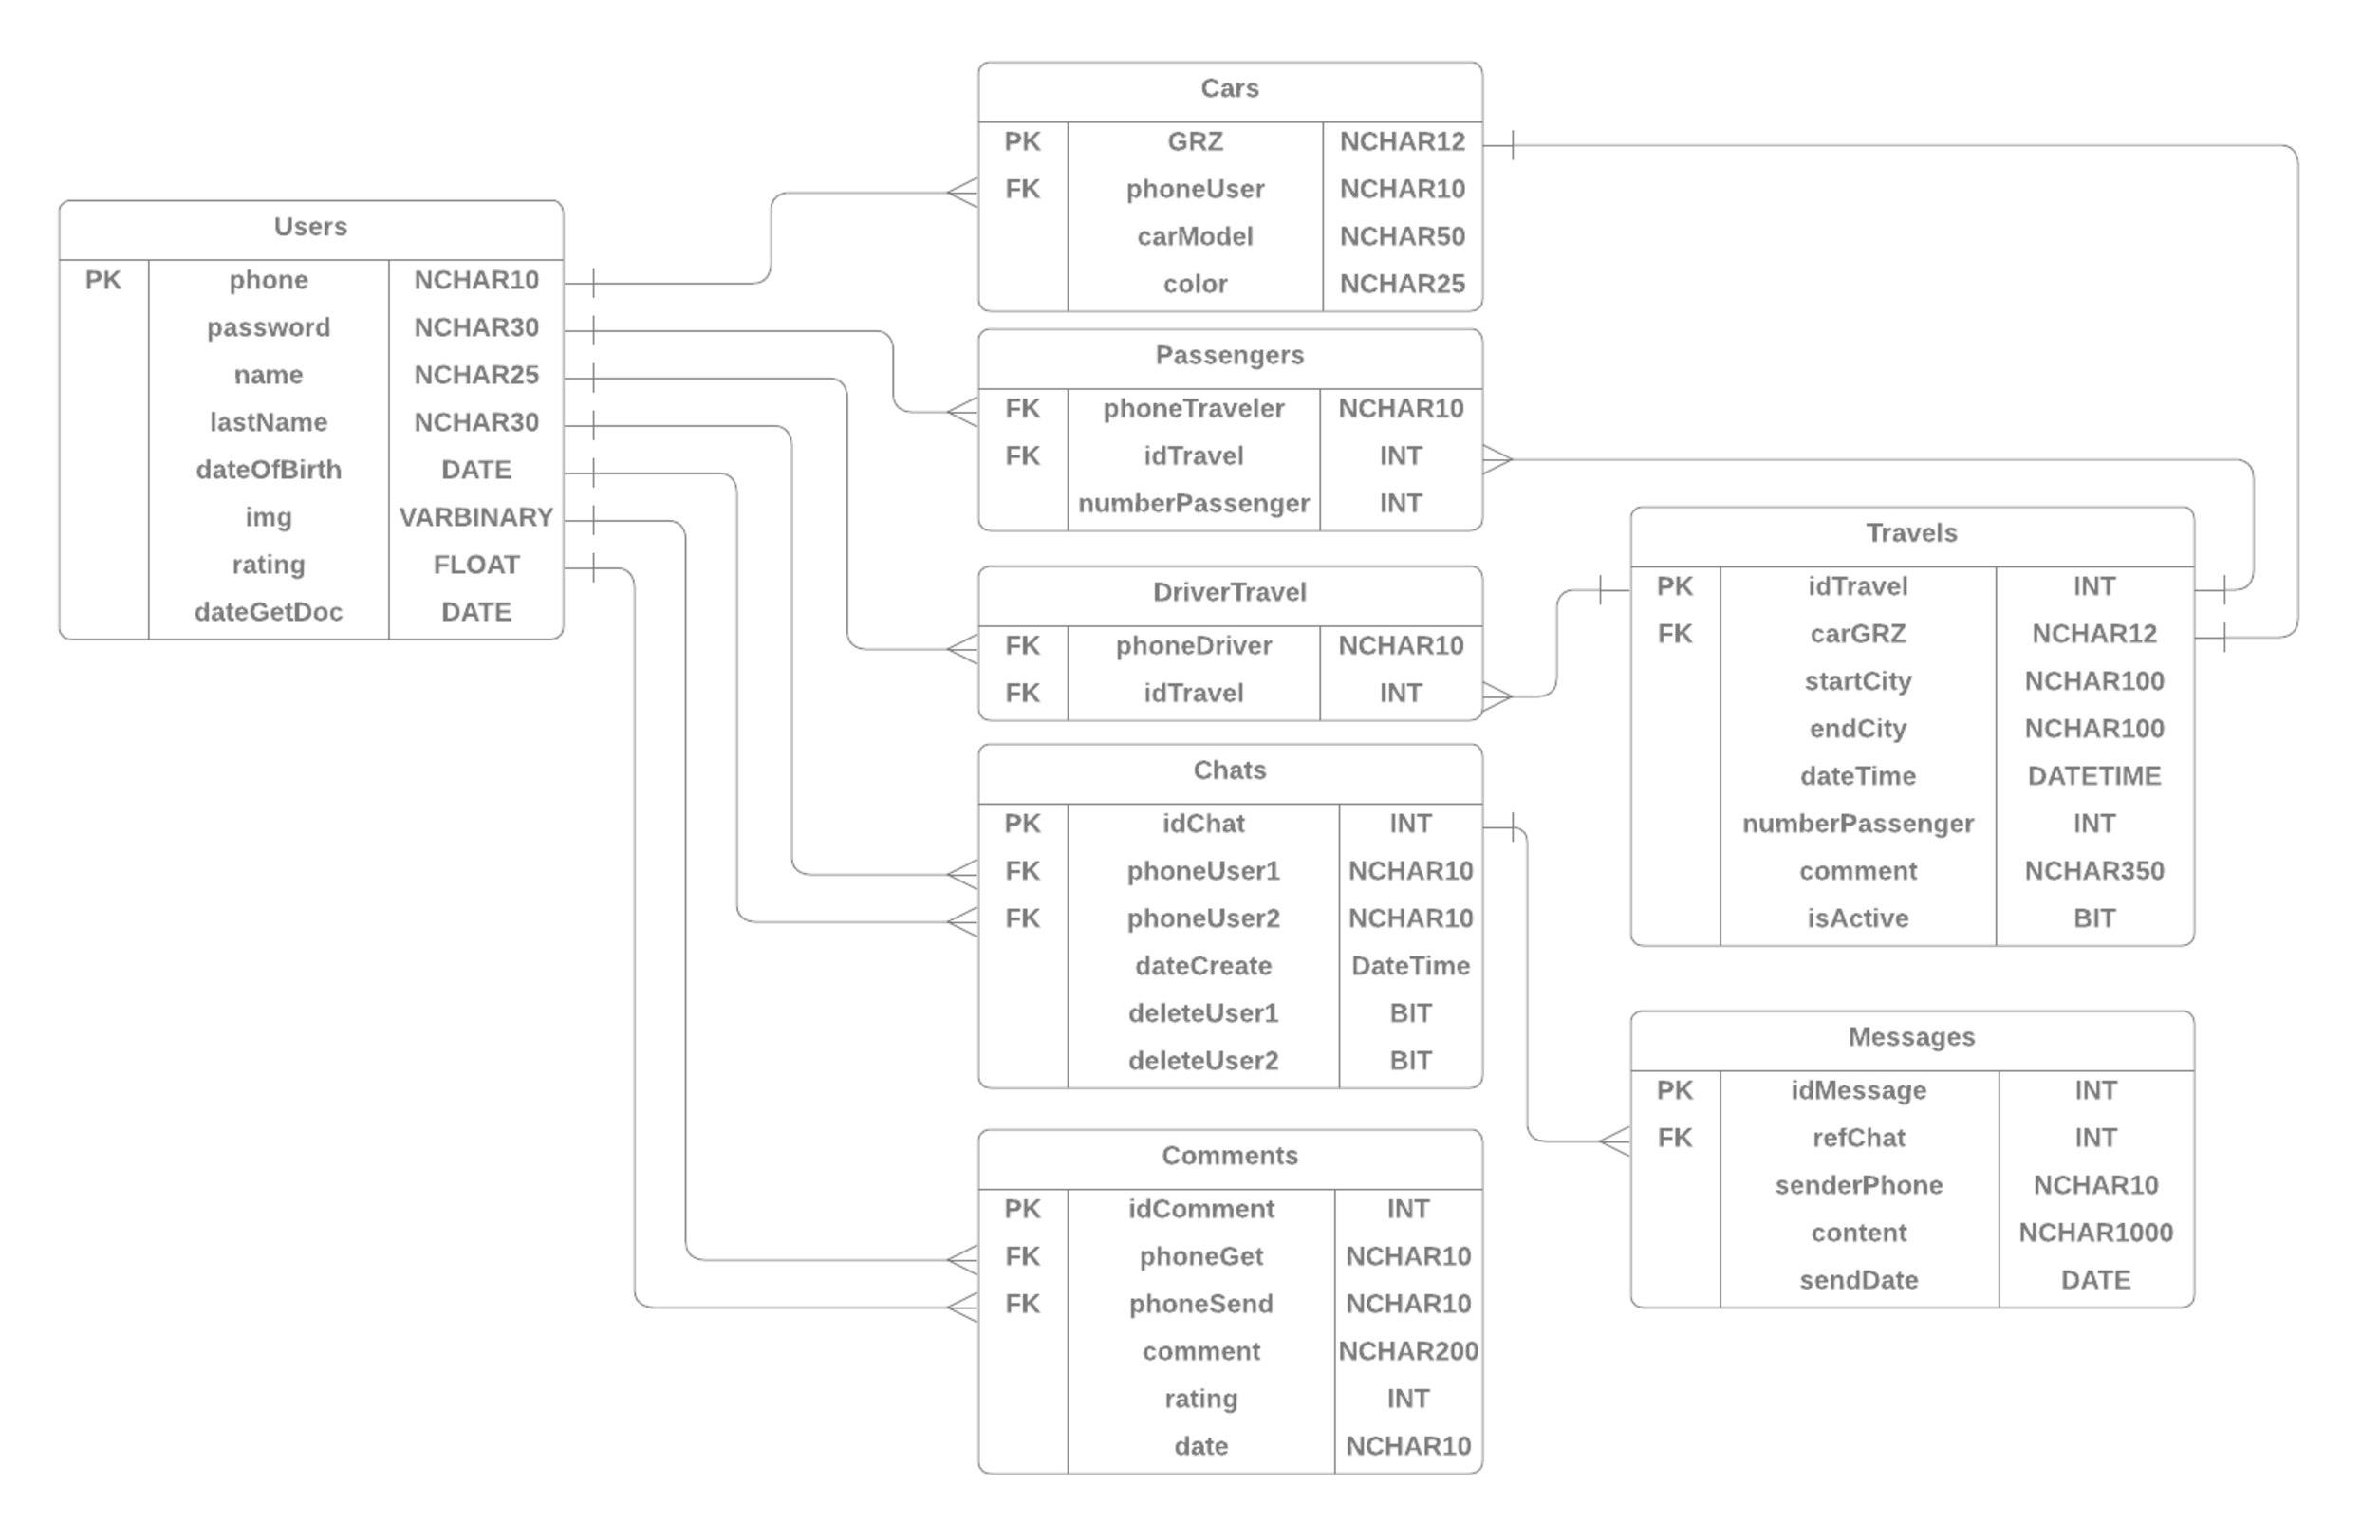
\includegraphics[width=0.9\linewidth]{images/ErDiagramDB}
	\caption{ER-диаграмма базы данных}
	\label{fig:erdiagramdb}
\end{figure}

В таблицах 3.1-3.8 представлены атрибуты таблиц базы данных.

\begin{xltabular}{\textwidth}{|X|X|X|}
	\caption{Атрибуты таблицы Users\label{ssevsws:table}}\\ \hline
	\centrow Название атрибута & \centrow Тип данных & \centrow Описание \\ \hline
	\endfirsthead
	\continuecaption{Продолжение таблицы \ref{ssevsws:table}}
	\centrow Название атрибута & \centrow Тип данных & \centrow Описание \\ \hline 
	\finishhead
	phone & NVARCHAR(10) & Номер телефона пользователя\\ \hline 
	password & NVARCHAR(30) & Пароль от учетной записи \\ \hline 
	name & NVARCHAR(25) & Имя пользователя \\ \hline 
	lastName & NVARCHAR(30) & Фамилия пользователя \\ \hline
	dateOfBirth & DATE & Дата рождения \\ \hline
	img & VARBINARY(MAX) & Фотография пользователя \\ \hline 
	rating & FLOAT & Рейтинг \\ \hline 
	dateGetDoc & DATE & Дата получения водительского удостоверения \\ \hline 
\end{xltabular}

\begin{xltabular}{\textwidth}{|X|X|X|}
	\caption{Атрибуты таблицы Cars\label{ssevsws:table}}\\ \hline
	\centrow Название атрибута & \centrow Тип данных & \centrow Описание \\ \hline
	\endfirsthead
	\continuecaption{Продолжение таблицы \ref{ssevsws:table}}
	\centrow Название атрибута & \centrow Тип данных & \centrow Описание \\ \hline 
	\finishhead
	GRZ & NVARCHAR(12) & Государственный регистрационный знак автомобиля \\ \hline 
	phoneUser & NVARCHAR(10) & FK на номер телефона \\ \hline 
	carModel & NVARCHAR(50) & Модель автомобиля \\ \hline 
	color & NVARCHAR(25) & Цвет автомобиля \\ \hline 
\end{xltabular}

\begin{xltabular}{\textwidth}{|X|X|X|}
	\caption{Атрибуты таблицы Passengers\label{ssevsws:table}}\\ \hline
	\centrow Название атрибута & \centrow Тип данных & \centrow Описание \\ \hline
	\endfirsthead
	\continuecaption{Продолжение таблицы \ref{ssevsws:table}}
	\centrow Название атрибута & \centrow Тип данных & \centrow Описание \\ \hline 
	\finishhead
	phoneTraveler & NVARCHAR(10) & FK на номер телефона попутчика \\ \hline 
	idTravel & INT & FK на уникальный идентификатор поездки \\ \hline 
	numberPassenger & INT & Количество пассажиров \\ \hline  
\end{xltabular}

\begin{xltabular}{\textwidth}{|X|X|X|}
	\caption{Атрибуты таблицы Travels\label{tb}}\\ \hline
	\centrow Название атрибута & \centrow Тип данных & \centrow Описание \\ \hline
	\endfirsthead
	\continuecaption{Продолжение таблицы \ref{tb}}
	\centrow Название атрибута & \centrow Тип данных & \centrow Описание \\ \hline 
	\finishhead
	idTravel & INT & Уникальнаый идентификатор поездки \\ \hline 
	carGRZ & NVARCHAR(12) & FK на ГРЗ автомобиля \\ \hline 
	startCity & NVARCHAR(100) & Город начала маршрута \\ \hline
	endCity & NVARCHAR(100) & Город окончания маршрута \\ \hline
	dateTime & DATETIME & Дата и время поездки \\ \hline
	numberPassenger & INT & Количество пассажиров в поездке \\ \hline
	comment & NVARCHAR(350) & Комментарий к поездке \\ \hline
	isActive & BIT & Статус активности \\ \hline  
\end{xltabular}

\begin{xltabular}{\textwidth}{|X|X|X|}
	\caption{Атрибуты таблицы DriverTravel\label{ssevsws:table}}\\ \hline
	\centrow Название атрибута & \centrow Тип данных & \centrow Описание \\ \hline
	\endfirsthead
	\continuecaption{Продолжение таблицы \ref{ssevsws:table}}
	\centrow Название атрибута & \centrow Тип данных & \centrow Описание \\ \hline 
	\finishhead
	phoneDriver & NVARCHAR(10) & FK на номер телефона водителя \\ \hline 
	idTravel & INT & FK на уникальный идентификатор поездки \\ \hline 
\end{xltabular}

\begin{xltabular}{\textwidth}{|X|X|X|}
	\caption{Атрибуты таблицы Chats\label{ssevsws:table}}\\ \hline
	\centrow Название атрибута & \centrow Тип данных & \centrow Описание \\ \hline
	\endfirsthead
	\continuecaption{Продолжение таблицы \ref{ssevsws:table}}
	\centrow Название атрибута & \centrow Тип данных & \centrow Описание \\ \hline 
	\finishhead
	idChat & INT & Уникальный идентификатор чата \\ \hline 
	phoneUser1 & NVARCHAR(10) & FK на номер телефона \\ \hline 
	phoneUser2 & NVARCHAR(10) & FK на номер телефона \\ \hline
	dateCreate & DateTime & Дата и время создания чата \\ \hline
	deleteUser1 & BIT & Статус удаленного чата у первого собесденика \\ \hline
	deleteUser2 & BIT & Статус удаленного чата у второго собесденика \\ \hline
\end{xltabular}

\begin{xltabular}{\textwidth}{|X|X|X|}
	\caption{Атрибуты таблицы Messages\label{ssevsws:table}}\\ \hline
	\centrow Название атрибута & \centrow Тип данных & \centrow Описание \\ \hline
	\endfirsthead
	\continuecaption{Продолжение таблицы \ref{ssevsws:table}}
	\centrow Название атрибута & \centrow Тип данных & \centrow Описание \\ \hline 
	\finishhead
	idMessage & INT & Уникальный идентификатор сообщения \\ \hline 
	refChat & INT & FK на чат \\ \hline 
	senderPhone & NVARCHAR(10) & Номер телефона отправителя \\ \hline
	content & NVARCHAR(1000) & Текст сообщения \\ \hline
	sendDate & DateTime & дата и время отправки \\ \hline
\end{xltabular}

\begin{xltabular}{\textwidth}{|X|X|X|}
	\caption{Атрибуты таблицы Comments\label{ssevsws:table}}\\ \hline
	\centrow Название атрибута & \centrow Тип данных & \centrow Описание \\ \hline
	\endfirsthead
	\continuecaption{Продолжение таблицы \ref{ssevsws:table}}
	\centrow Название атрибута & \centrow Тип данных & \centrow Описание \\ \hline 
	\finishhead
	idComment & INT & Уникальный идентификатор комментария \\ \hline 
	phoneGet & NVARCHAR(10) & Телефон получателя \\ \hline 
	phoneSend & NVARCHAR(10) & Телефон отправителя \\ \hline
	comment & NVARCHAR(200) & Текст комментария \\ \hline
	rating & INT & Оценка \\ \hline
	date & DATE & Дата комментария \\ \hline 
\end{xltabular}

\subsection{Проектирование архитектуры программной системы}
\subsubsection{Компоненты программной системы}

Разрабатываемая система представляет из себя серверное приложение.
Для разработки backend-модуля будет использоваться язык программирования C\# 10.0{[40]} с применением фреймворка ASP.Net для создания серверного модуля и фреймворка SqlClient{[39]} для обеспечения доступа к базе данных.

Используемая среда разработки – Visual Studio 2022.

В качестве СУБД необходимо использовать Microsoft SQL Server.

В качестве системы управления версиями для командной разработки необходимо использовать Git{[41]}{[42]}{[43]}.

Диаграмма развёртывания программы представлена на рисунке 3.2

\begin{figure}[H]
	\centering
	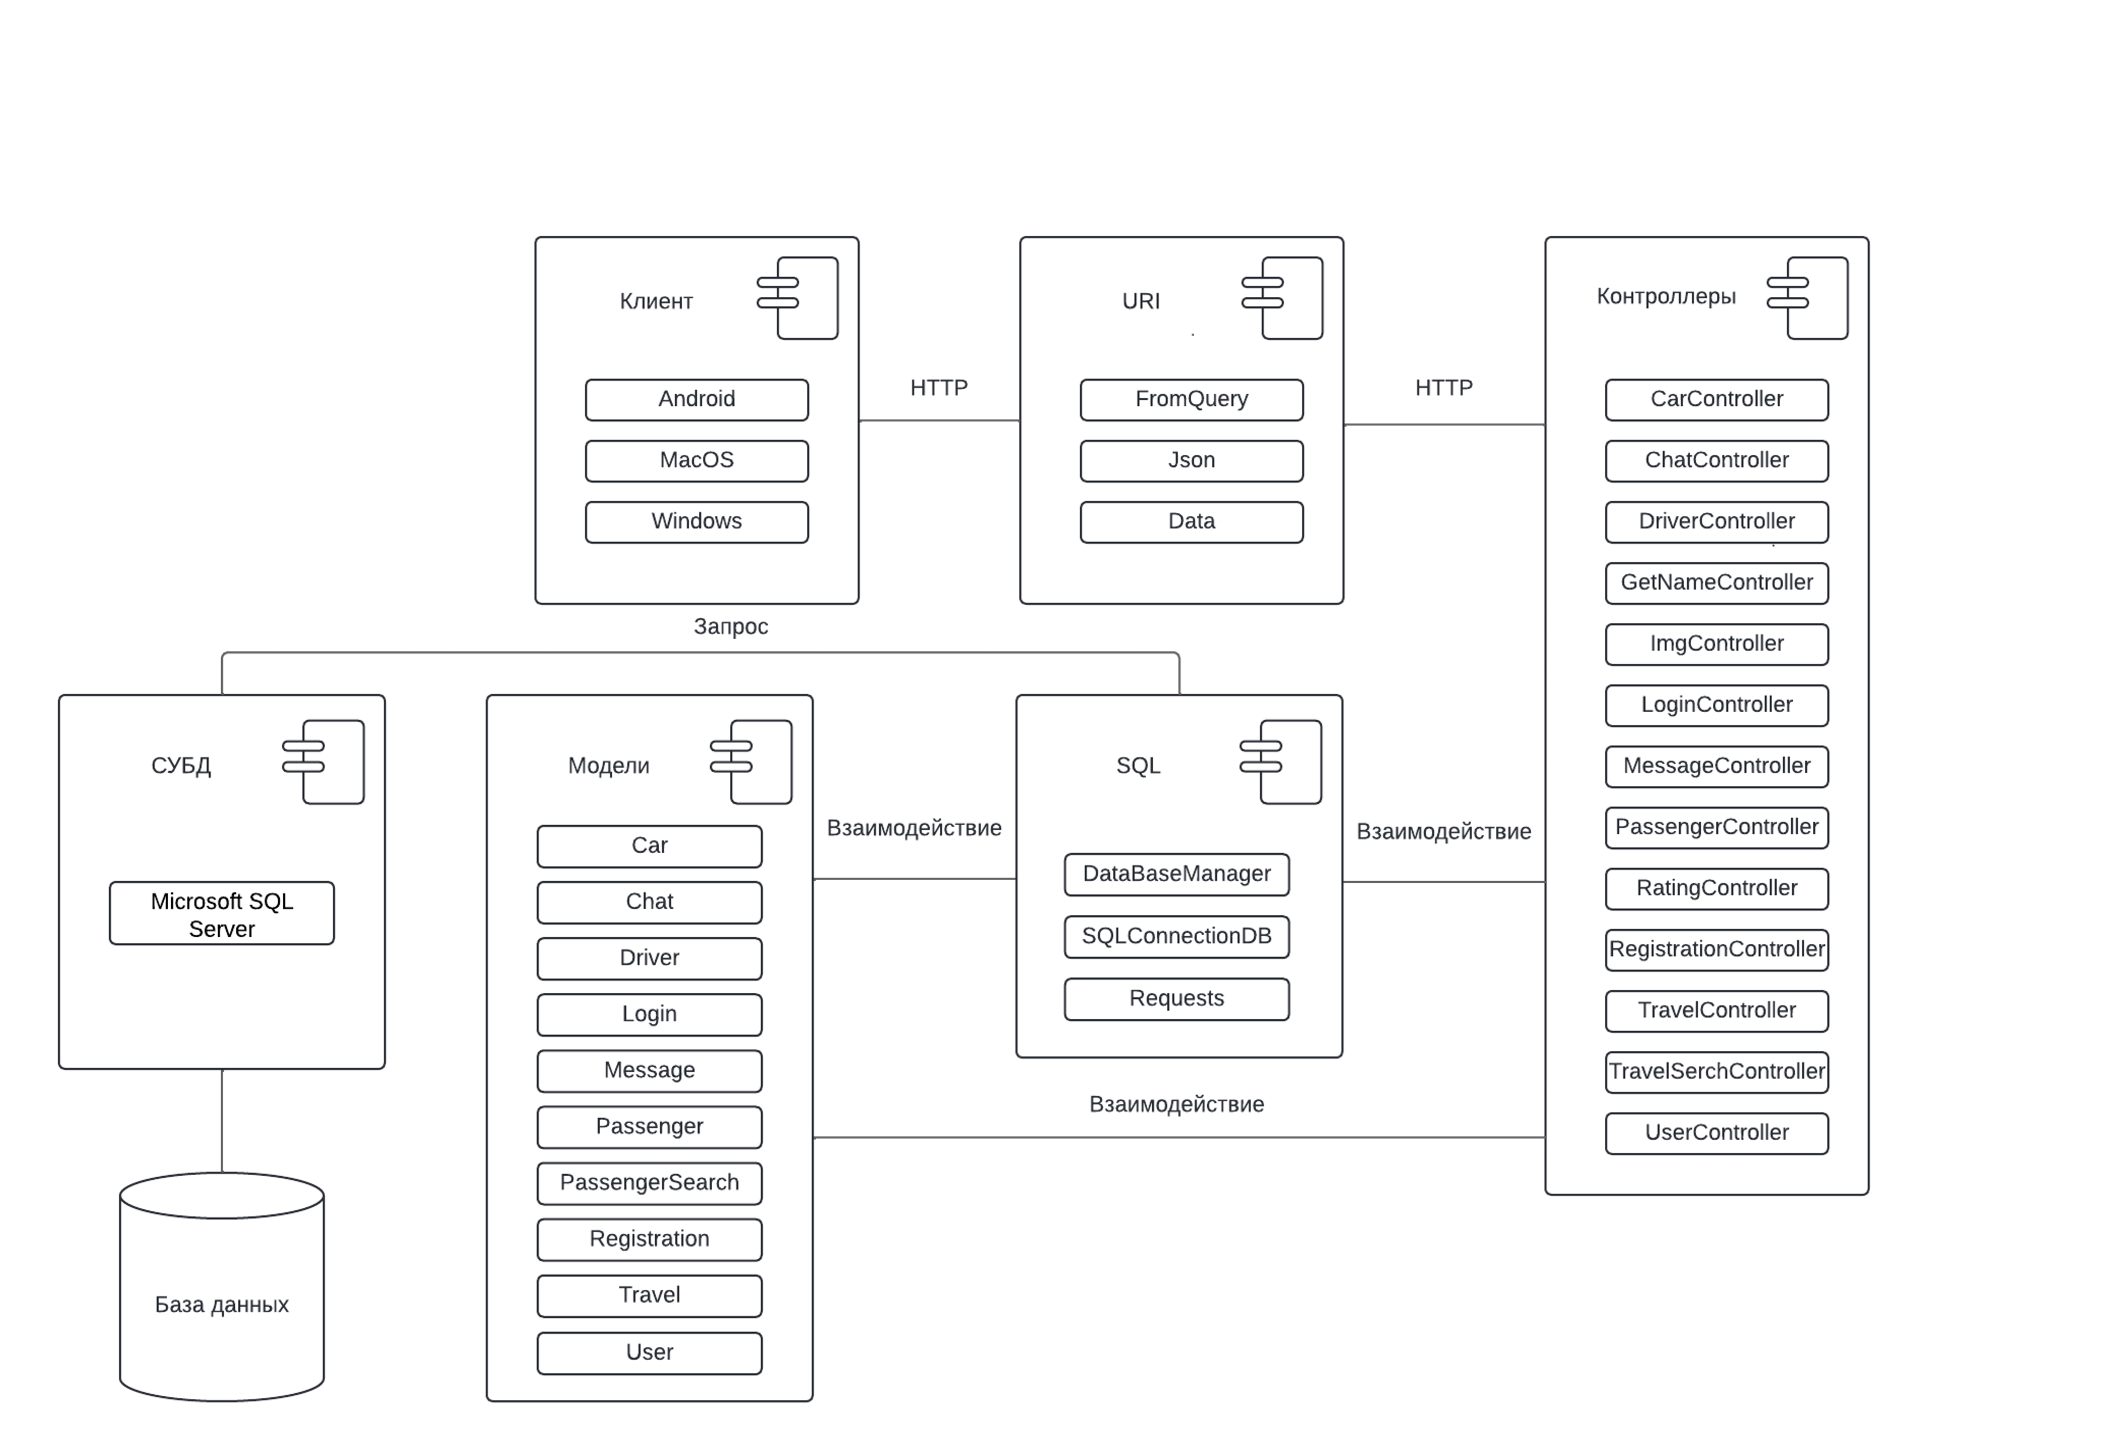
\includegraphics[width=0.9\linewidth]{images/diagramArch}
	\caption{Диаграмма развертывания программы}
	\label{fig:diagramarch}
\end{figure}

Программно-информационная система состоит из нескольких ключевых компонентов, каждый из которых выполняет свои уникальные функции, обеспечивая бесперебойную работу всей платформы. В центре этой системы находится клиентская часть, представленная приложениями для различных операционных систем, таких как Android, MacOS и Windows. Эти приложения позволяют пользователям взаимодействовать с системой через HTTP-запросы, обеспечивая доступ к необходимым функциям и данным.

Одним из важнейших компонентов системы является URI, который обрабатывает запросы, поступающие от клиентов. URI играет ключевую роль в маршрутизации и управлении данными, обрабатывая параметры запросов, работая с JSON-данными[{44}][{45}] и управляя передаваемыми данными. Благодаря этому компоненту, система может эффективно и безопасно обмениваться информацией между клиентами и серверами. URI, в свою очередь, направляет запросы к соответствующим контроллерам, которые отвечают за выполнение конкретных задач.

Контроллеры представляют собой еще один важный элемент системы. Они отвечают за выполнение различных операций, связанных с функциональностью системы. Контроллеры управляют данными о транспортных средствах, чатами между пользователями, информацией о водителях, а также процессами аутентификации и регистрации пользователей. Они также занимаются управлением сообщениями, пассажирами, рейтингами, поездками и данными пользователей, обеспечивая координацию и выполнение всех основных функций системы. Каждый запрос, поступающий от клиента через URI, направляется к соответствующему контроллеру для обработки и выполнения необходимых операций.

Модели представляют собой набор компонентов, которые описывают основные сущности системы. Они включают в себя такие важные элементы, как транспортные средства, чаты, водители, пассажиры, поездки и пользователи. Эти модели играют ключевую роль в взаимодействии с базой данных, обеспечивая структурированный и организованный подход к хранению и обработке данных. Взаимодействие моделей с базой данных осуществляется через слой SQL, который включает в себя управление базой данных, установление и управление соединениями, а также обработку запросов к базе данных. Контроллеры взаимодействуют с моделями для выполнения операций чтения и записи данных, обеспечивая тем самым актуальность и консистентность данных в системе.

СУБД, используемая в системе, представлена Microsoft SQL Server. Эта система управления базами данных обеспечивает надежное и эффективное хранение всех данных, необходимых для работы платформы. Взаимодействие с базой данных осуществляется через SQL-компоненты, что позволяет обеспечить высокую производительность и надежность при работе с большими объемами данных. Модели обращаются к SQL для выполнения операций с данными, таких как запросы, обновления и удаления, гарантируя, что все данные, хранящиеся в базе данных, актуальны и доступны для обработки.

Таким образом, программно-информационная система представляет собой сложную и многоуровневую структуру, включающую в себя клиентскую часть, URI, контроллеры, модели, слой SQL и СУБД. Взаимодействие между этими компонентами осуществляется через четко определенные интерфейсы и протоколы, обеспечивая функциональность, надежность и безопасность всей платформы. Клиентские приложения отправляют запросы через URI, который маршрутизирует их к соответствующим контроллерам. Контроллеры, в свою очередь, взаимодействуют с моделями и SQL для выполнения необходимых операций с данными. Все данные хранятся в надежной СУБД, обеспечивая целостность и доступность информации. Взаимодействие между этими компонентами позволяет системе эффективно выполнять свои задачи и обеспечивать пользователям доступ к необходимым данным и функциям.

\subsubsection{Архитектура программной системы}

Архитектура MVC (Model-View-Controller) является широко распространенной парадигмой проектирования программного обеспечения, которая способствует разделению приложения на три взаимосвязанных компонента: модель, представление и контроллер. Эта архитектура позволяет улучшить управляемость, модульность и тестируемость кода.

Модель (Model)

Модель отвечает за управление данными и бизнес-логикой приложения. Она представляет собой центральную часть архитектуры, где происходят все операции с данными. Модель определяет структуру данных, правила их обработки и взаимодействие с базами данных или другими источниками данных. В модели реализуются основные функции, такие как получение, сохранение, обновление и удаление данных. Модель также уведомляет представление о необходимости обновления данных, чтобы обеспечить синхронизацию между состоянием данных и их отображением.

Представление (View)

Представление отвечает за отображение данных пользователю. Оно получает данные от модели и отображает их в удобной и понятной форме. Представление не содержит логики обработки данных; его задача — только визуализация информации. В веб-приложениях это могут быть HTML-страницы, шаблоны или компоненты пользовательского интерфейса. Важно отметить, что представление не взаимодействует напрямую с моделью, а получает данные через контроллер, что способствует снижению зависимости между компонентами.

Контроллер (Controller)

Контроллер служит посредником между моделью и представлением. Он обрабатывает входные данные от пользователя, вызывает соответствующие методы модели для обработки этих данных и обновляет представление в соответствии с результатами работы модели. Контроллеры принимают запросы от пользователей, определяют, какие действия должны быть выполнены, и управляют потоком данных между моделью и представлением. Благодаря этому контроллеры обеспечивают логическую связь между компонентами системы и позволяют изолировать бизнес-логику от пользовательского интерфейса.

Взаимодействие между компонентами:

\begin{itemize}
	\item Модель и Представление. Модель обновляет данные и уведомляет представление о необходимости изменения отображения. Представление запрашивает данные у модели и обновляется в соответствии с изменениями.
	\item Модель и Контроллер. Контроллер взаимодействует с моделью для выполнения операций над данными. Он отправляет запросы модели на изменение данных и получает обновленные данные для последующей передачи представлению.
	\item Контроллер и Представление. Контроллер управляет отображением данных, передавая модели необходимые запросы и обновляя представление в соответствии с результатами работы модели. Контроллер обрабатывает пользовательские запросы и определяет, какие действия нужно предпринять, чтобы ответить на эти запросы.
\end{itemize}

Преимущества архитектуры MVC:

\begin{itemize}
	\item Разделение обязанностей. Разделение кода на три компонента улучшает управляемость и упрощает сопровождение приложения.
	\item Модульность. Каждый компонент можно разрабатывать и тестировать независимо от других, что ускоряет процесс разработки.
	\item Повышенная тестируемость. Благодаря четкому разделению обязанностей проще писать и выполнять автоматические тесты для каждого компонента.
	\item Масштабируемость. Архитектура MVC облегчает добавление новых функций и компонентов без значительного изменения существующего кода.
	\item Гибкость. Легче менять или обновлять отдельные компоненты системы, такие как пользовательский интерфейс, не затрагивая бизнес-логику.
\end{itemize}

Архитектура MVC, благодаря своему структурированному подходу и разделению обязанностей, помогает создавать более надежные, поддерживаемые и масштабируемые приложения.

\subsubsection{Архитектура программных классов моделей и контроллеров}

IActionResult - это интерфейс, который представляет результат действия в ASP.NET Core. Контроллеры возвращают объекты, реализующие этот интерфейс, чтобы сообщить о результате выполнения запроса. Например, это может быть возвращение данных, сообщение об ошибке или перенаправление.

На рисунке 3.3 представлена UML-диаграмма классов программной системы, отражающих взаимодействие моделей и контроллеров.

\begin{figure}[H]
	\centering
	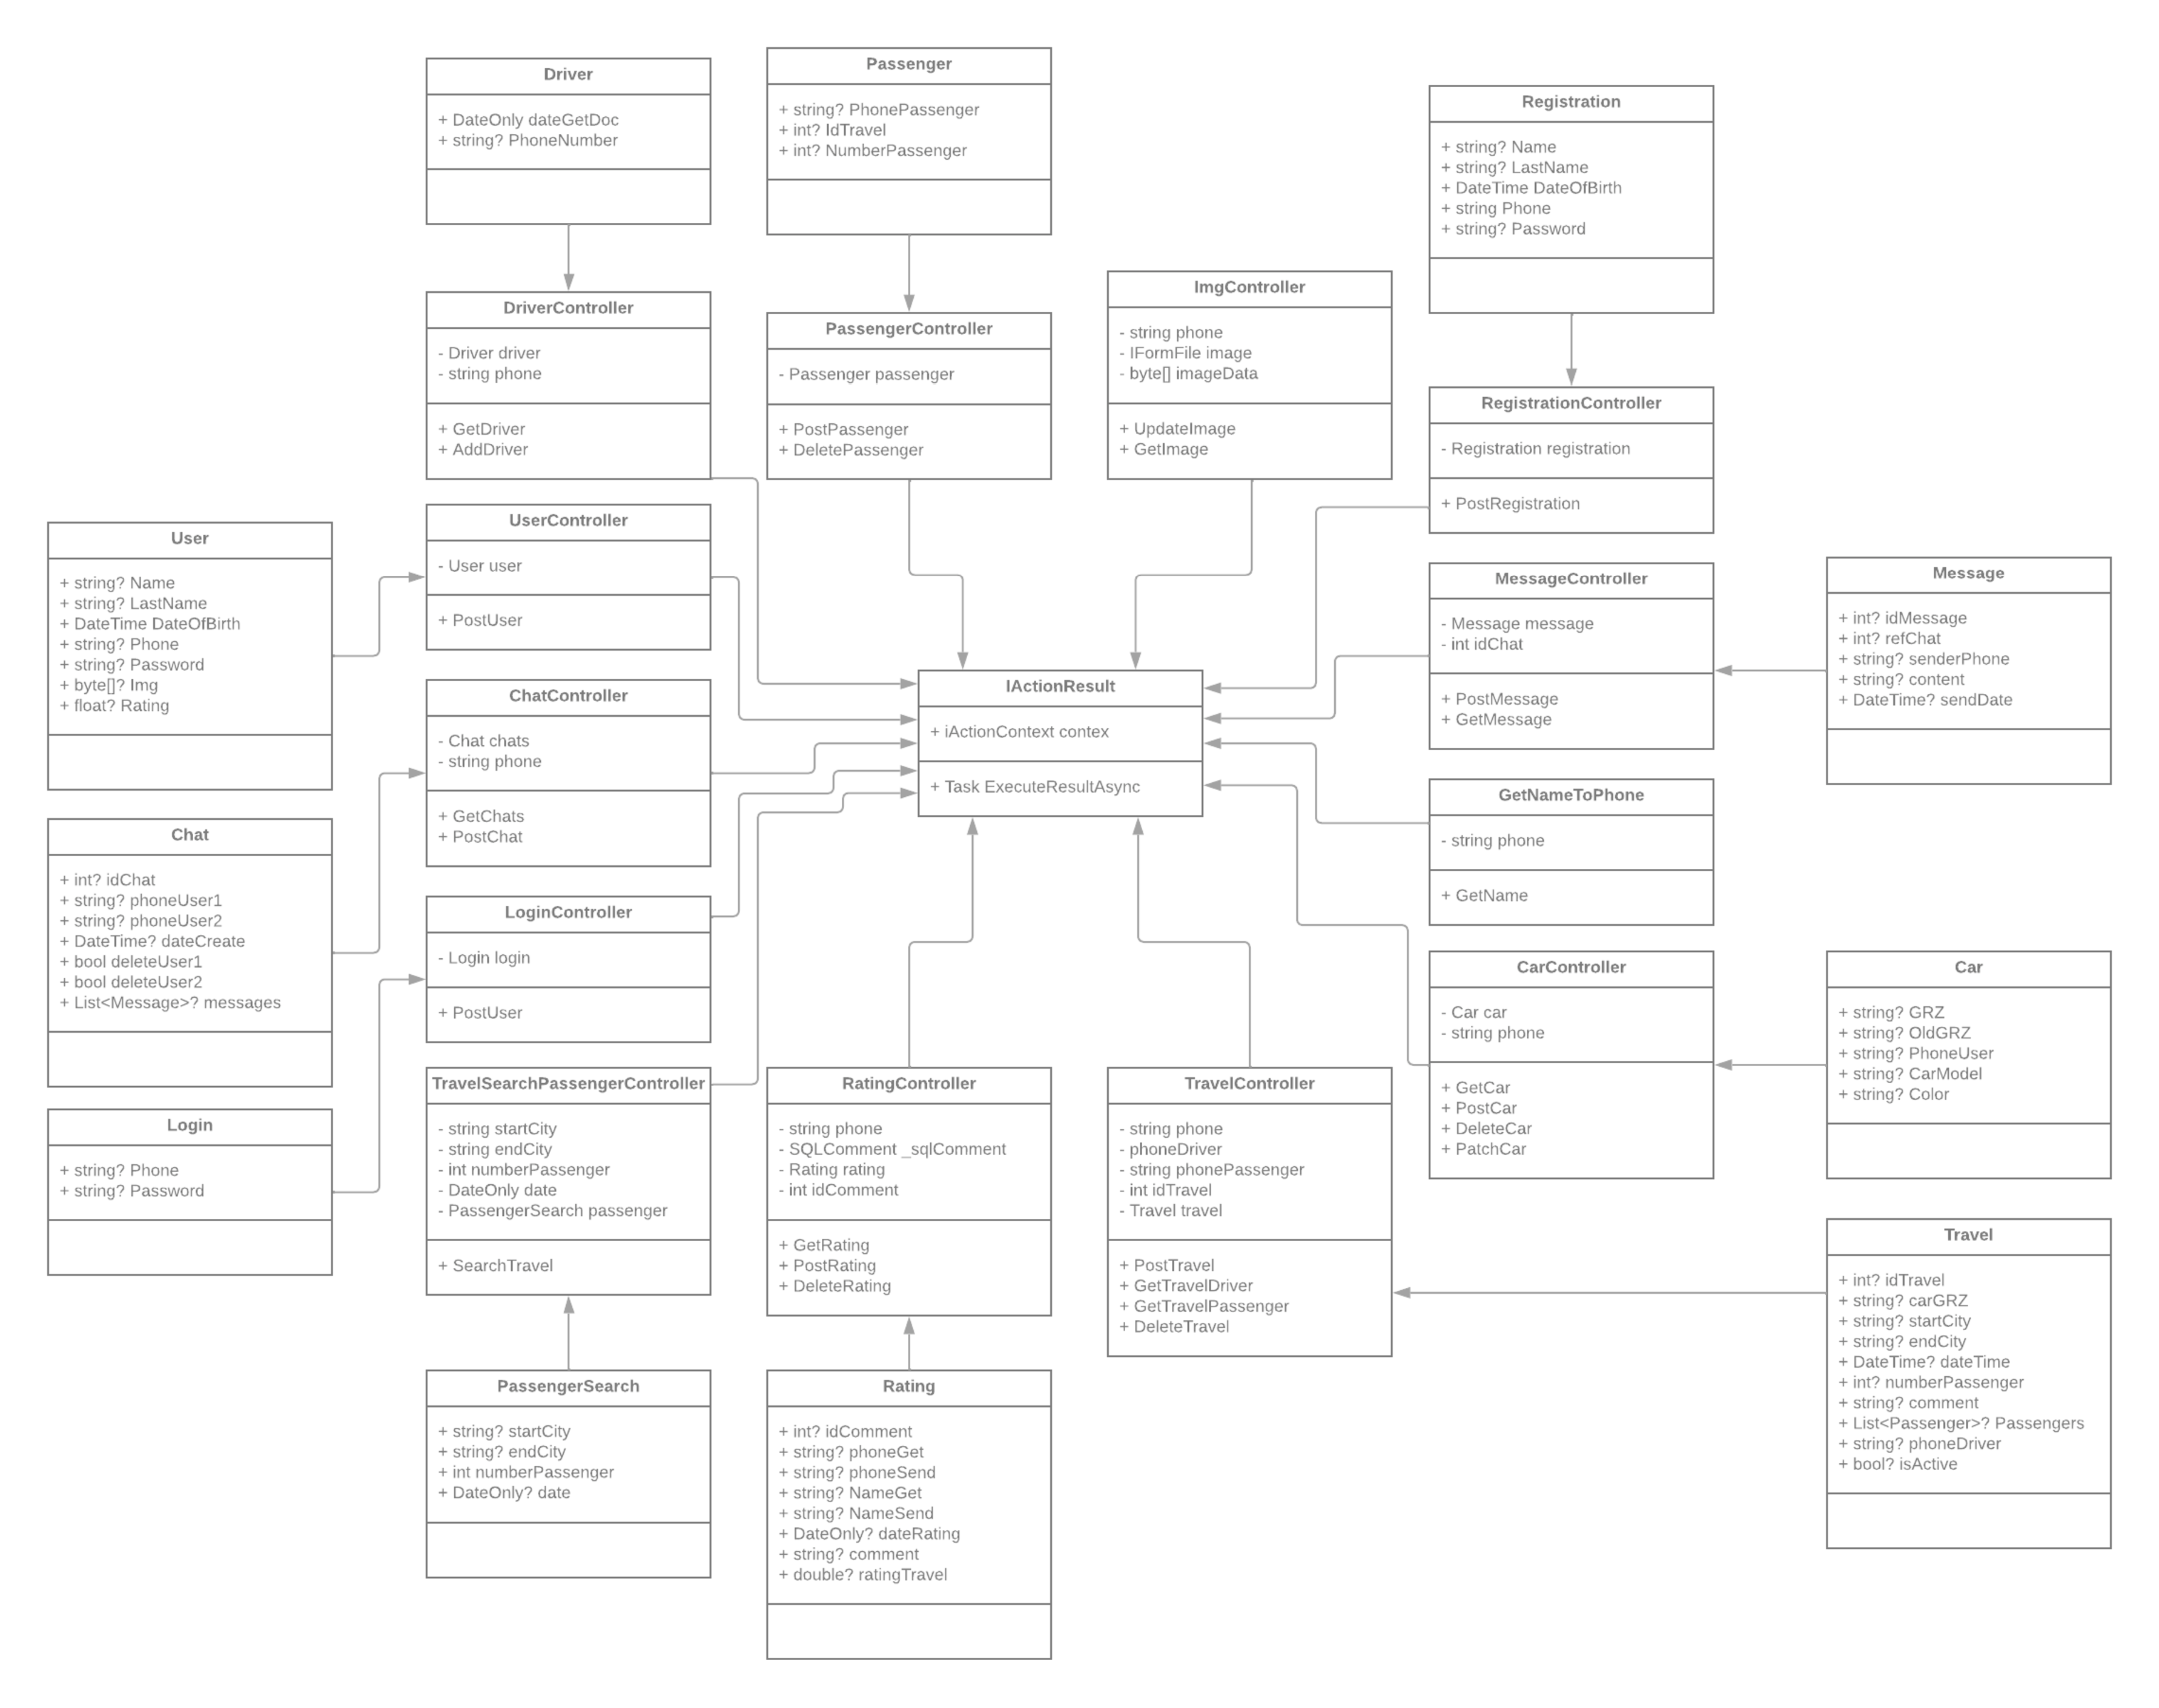
\includegraphics[width=0.9\linewidth]{images/DiagramArch2}
	\caption{Диаграмма классов моделей и контроллеров}
	\label{fig:diagramarch2}
\end{figure}

Driver (Водитель) -- хранит информацию о водителях.

Passenger (Пассажир) -- содержит данные о пассажирах.

User (Пользователь) -- включает основную информацию о пользователях системы.

Chat (Чат) -- содержит информацию о чатах между пользователями.

Login (Логин) -- хранит данные для входа в систему.

Registration (Регистрация) -- содержит информацию для регистрации новых пользователей.

Message (Сообщение) -- представляет сообщения в чатах.

Car (Автомобиль) -- включает данные об автомобилях пользователей.

Travel (Поездка) -- содержит информацию о поездках.

PassengerSearch (Поиск пассажиров) -- используется для поиска пассажиров.

Rating (Рейтинг) -- включает данные о рейтингах пользователей.

DriverController (Контроллер водителей) -- управляет операциями, связанными с водителями.

PassengerController (Контроллер пассажиров) -- обрабатывает операции, связанные с пассажирами.

UserController (Контроллер пользователей) -- управляет действиями, связанными с пользователями.

ChatController (Контроллер чатов) -- управляет взаимодействиями в чатах.

LoginController (Контроллер входа) -- обрабатывает операции входа в систему.

RegistrationController (Контроллер регистрации) -- управляет регистрацией новых пользователей.

MessageController (Контроллер сообщений) -- обрабатывает операции, связанные с сообщениями в чатах.

GetNameToPhone (Контроллер получения имени по телефону) -- предоставляет функциональность получения имени по номеру телефона.

CarController (Контроллер автомобилей) -- управляет данными об автомобилях.

TravelController (Контроллер поездок) -- обрабатывает операции, связанные с поездками.

TravelSearchPassengerController (Контроллер поиска пассажиров для поездок) -- управляет поиском пассажиров для поездок.

RatingController (Контроллер рейтингов) -- управляет данными о рейтингах.


\subsubsection{Архитектура программных классов SQL запросов}

SQLConnectionDb предоставляет стандартные параметры для подключения к базе данных. Этот класс отвечает за установку и хранение параметров подключения, таких как строка подключения и настройки, необходимые для подключения к базе данных.

SqlConnection представляет подключение к базе данных и управляет его состоянием. Это класс от Microsoft, который обеспечивает методы для открытия и закрытия соединения, а также выполнения команд SQL.

DatabaseManager предоставляет асинхронные методы для работы с базой данных. Этот класс управляет открытием и закрытием подключений в асинхронном режиме, что позволяет повысить производительность системы за счет эффективного использования ресурсов и предотвращения блокировок.

На рисунке 3.4 представлена UML-диаграмма классов программной системы, отражающих принцип работы SQL запросов.

\begin{figure}[H]
	\centering
	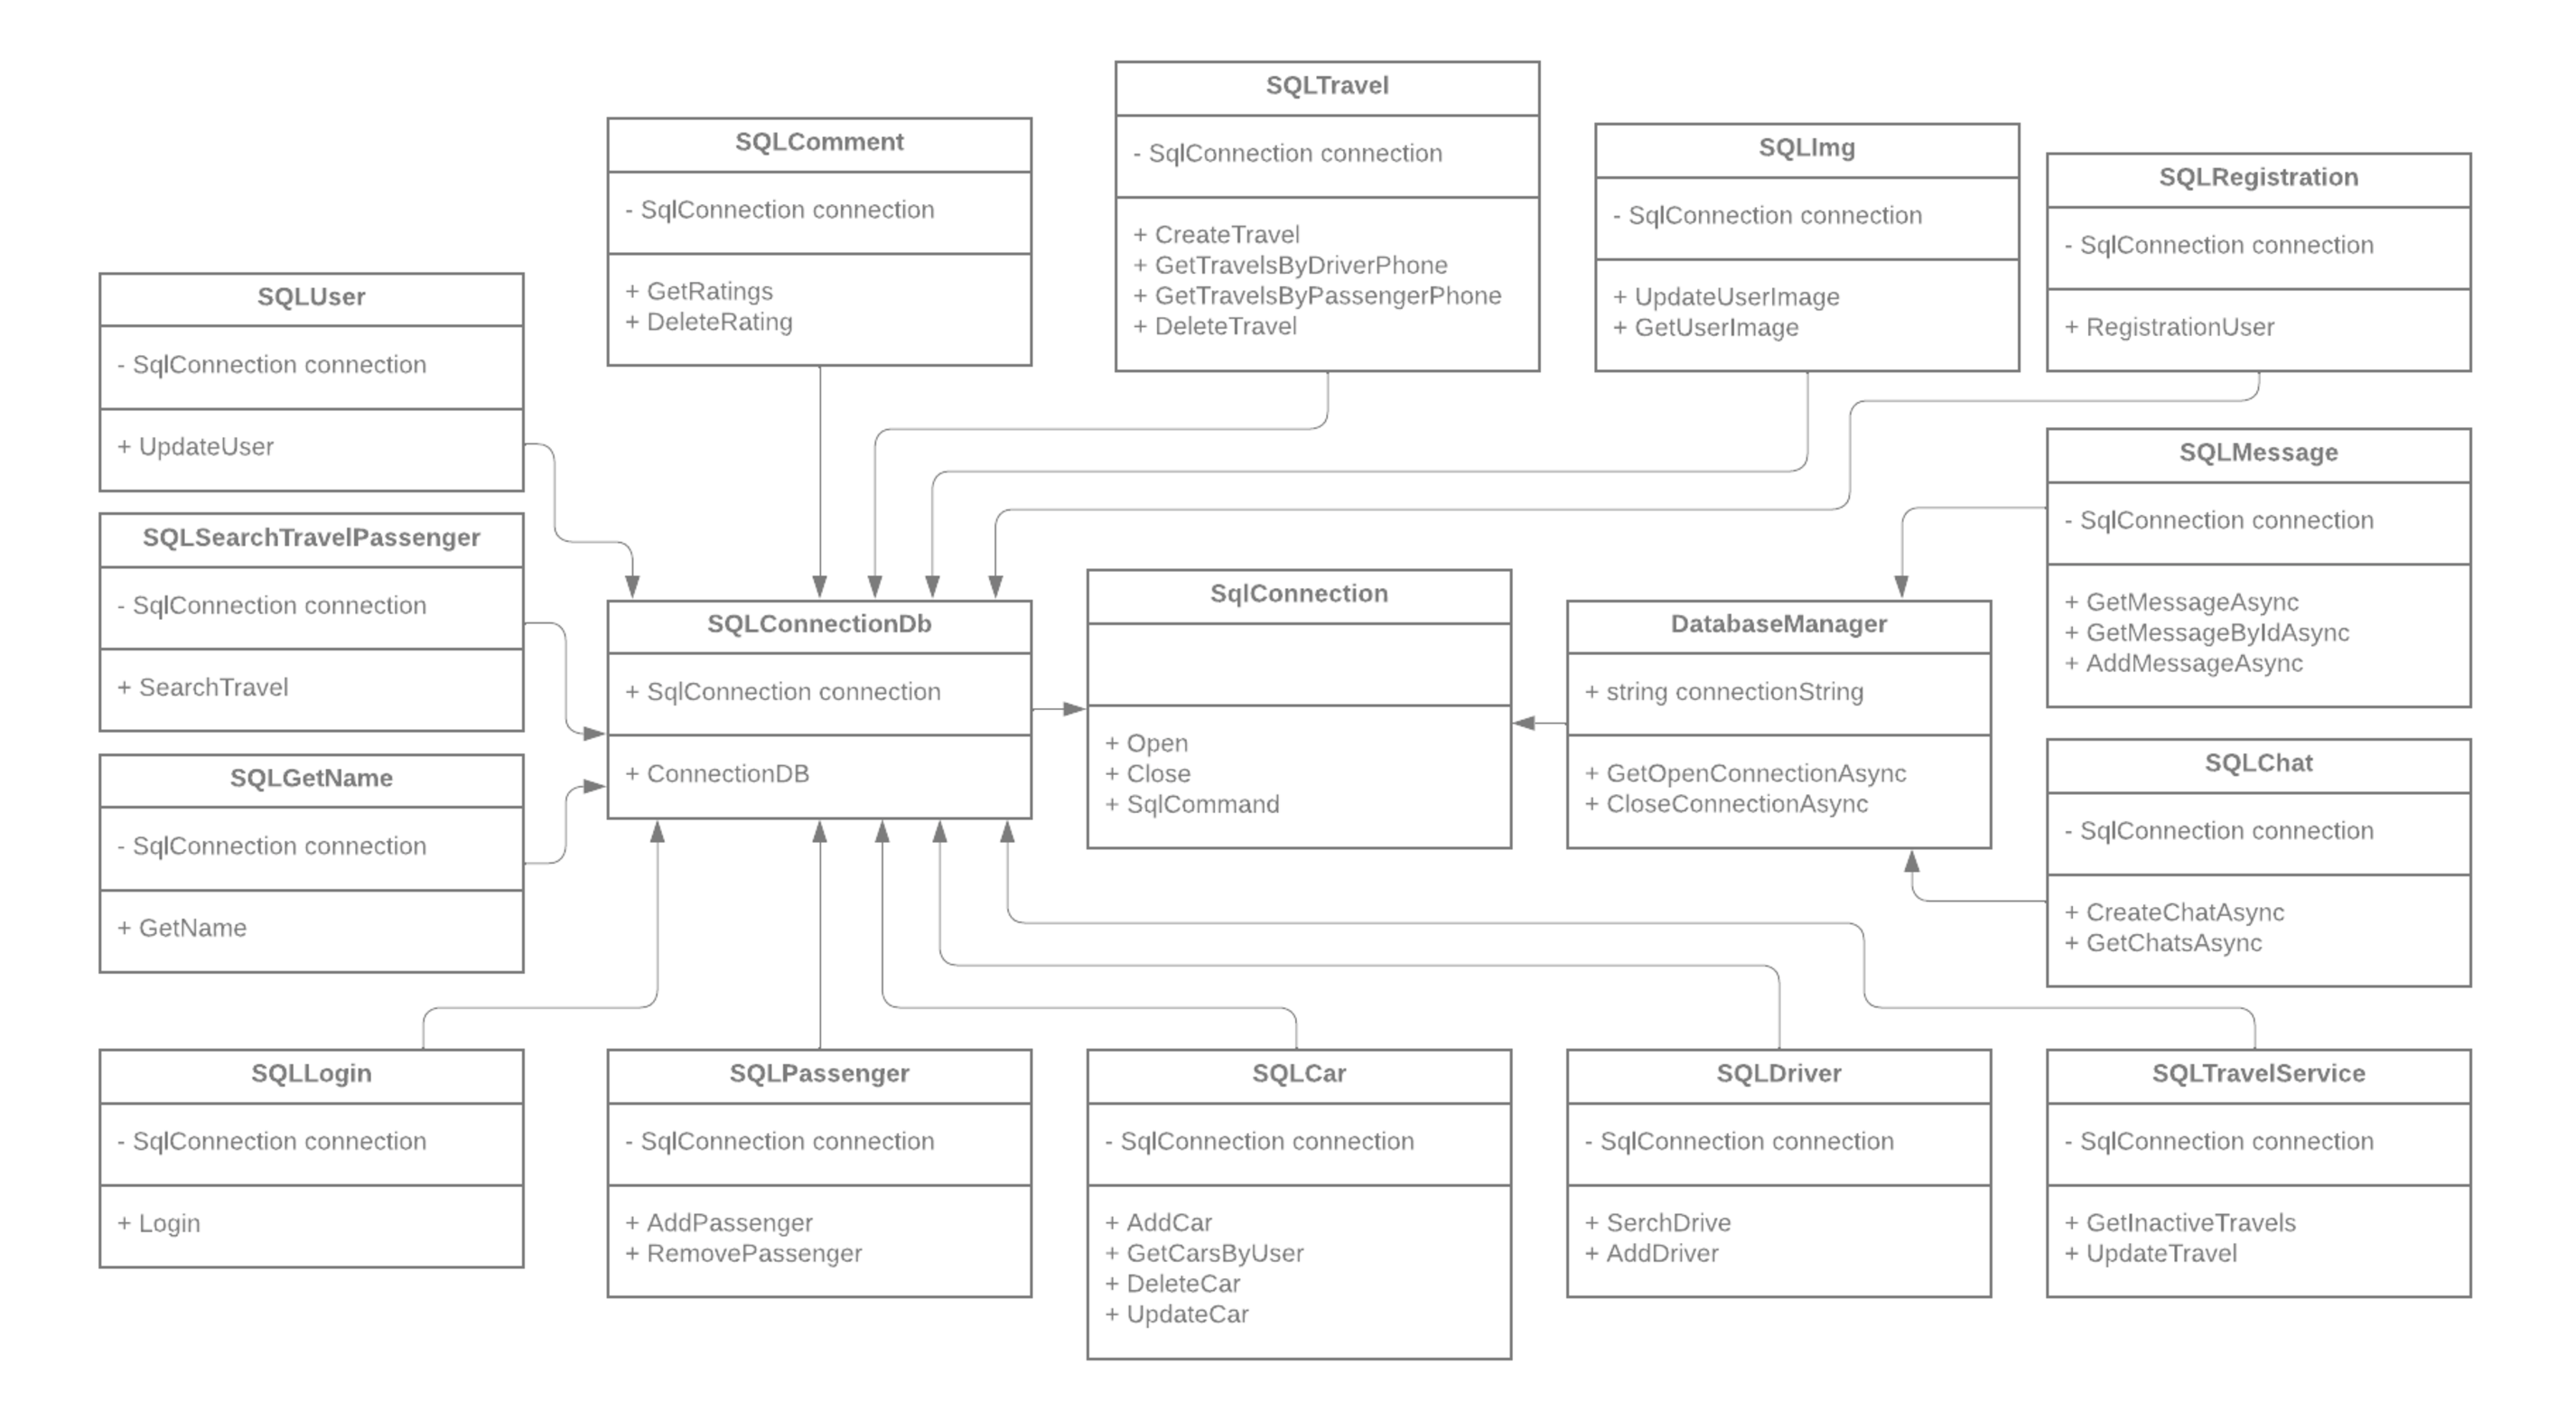
\includegraphics[width=0.9\linewidth]{images/DiagramArch3}
	\caption{Диаграмма классов SQL запросов}
	\label{fig:diagramarch3}
\end{figure}

SQLUser позволяет обновлять информацию о пользователях.

SQLSearchTravelPassenger обеспечивает функциональность поиска пассажиров для поездок.

SQLGetName позволяет получать имя пользователя по номеру телефона.

SQLLogin управляет операциями входа в систему.

SQLPassenger позволяет добавлять и удалять пассажиров.

SQLCar управляет данными об автомобилях, включая добавление, получение, удаление и обновление информации о них.

SQLDriver обеспечивает поиск и добавление водителей.

SQLTravel управляет данными о поездках, включая создание, получение и удаление поездок.

SQLImg позволяет обновлять и получать изображения пользователей.

SQLRegistration управляет регистрацией новых пользователей.

SQLMessage обеспечивает функциональность для работы с сообщениями в чатах, включая их получение и добавление.

SQLChat управляет созданием чатов и получением списка чатов.

SQLTravelService обеспечивает дополнительные сервисы для работы с поездками, такие как получение неактивных поездок и обновление информации о поездках.

SQLComment управляет данными о рейтингах и комментариях, включая их получение и удаление.

\ifПрактика{}\else{
   \section{Рабочий проект}
\subsection{Классы, используемые при разработке серверной части программной системы}

В данном разделе описывается список классов и их методов, использованных при разработке серверной части программной системы. 

\subsubsection{Спецификация классов SQL запросов}

Основные SQL-классы для подключения к базе данных включают SQLConnectionDb и DatabaseManager. 

SQLConnectionDb предоставляет методы для управления соединением с базой данных, включая открытие, закрытие и проверку состояния соединения. Этот класс используется для синхронного взаимодействия с базой данных.

DatabaseManager - это асинхронная версия класса подключения к базе данных, которая обеспечивает возможность выполнения асинхронных запросов к базе данных для улучшения производительности и масштабируемости. Он предоставляет асинхронные версии методов для работы с соединением, что позволяет выполнять асинхронные операции базы данных без блокировки потока.

В таблицах 4.1 -- 4.19 приведено описание полей и методов классов для работы с базой данных.

\renewcommand{\arraystretch}{0.8} % уменьшение расстояний до сетки таблицы
\begin{xltabular}{\textwidth}{|X|p{3cm}|p{3cm}|>{\setlength{\baselineskip}{0.7\baselineskip}}p{4.85cm}|}
	\caption{Спецификация полей класса «SQLConnectionDb» \label{class1:table}}\\
	\hline \centrow \setlength{\baselineskip}{0.7\baselineskip} Наименование & \centrow \setlength{\baselineskip}{0.7\baselineskip} Метод доступа & \centrow Тип данных & \centrow Описание \\
	\hline \centrow 1 & \centrow 2 & \centrow 3 & \centrow 4\\ \hline
	\endfirsthead
	\continuecaption{Продолжение таблицы \ref{class1:table}}
	\centrow 1 & \centrow 2 & \centrow 3 & \centrow 4\\ \hline
	\finishhead
	connectionString & private & string? & Строка подключения к БД \\ \hline 
	connection & protected & SqlConnection & Состояние подключения к БД \\ \hline 
\end{xltabular}
\renewcommand{\arraystretch}{1.0} % восстановление сетки

\renewcommand{\arraystretch}{0.8} % уменьшение расстояний до сетки таблицы
\begin{xltabular}{\textwidth}{|p{4cm}|p{3cm}|>{\setlength{\baselineskip}{0.7\baselineskip}}X|}
	\caption{Спецификация методов класса «SQLConnectionDb» \label{class2:table}}\\
	\hline \centrow \setlength{\baselineskip}{0.7\baselineskip} Наименование & \centrow \setlength{\baselineskip}{0.7\baselineskip} Метод доступа & \centrow Описание \\
	\hline \centrow 1 & \centrow 2 & \centrow 3\\ \hline
	\endfirsthead
	\continuecaption{Продолжение таблицы \ref{class2:table}}
	\centrow 1 & \centrow 2 & \centrow 3\\ \hline
	\finishhead
	ConnectionDB & public & Устанавливает соединение с базой данных, используя заданную строку подключения. В случае успеха возвращает объект типа SqlConnection, представляющий активное соединение. В случае ошибки выводит сообщение об ошибке и возвращает null.\\ \hline 
	CloseDB & public & Закрывает текущее соединение с базой данных. Не принимает аргументов. Возвращает объект типа SqlConnection, представляющий закрытое соединение.\\ \hline 
\end{xltabular}
\renewcommand{\arraystretch}{1.0} % восстановление сетки

\renewcommand{\arraystretch}{0.8} % уменьшение расстояний до сетки таблицы
\begin{xltabular}{\textwidth}{|X|p{3cm}|p{3cm}|>{\setlength{\baselineskip}{0.7\baselineskip}}p{4.85cm}|}
	\caption{Спецификация полей класса «DatabaseManager» \label{class3:table}}\\
	\hline \centrow \setlength{\baselineskip}{0.7\baselineskip} Наименование & \centrow \setlength{\baselineskip}{0.7\baselineskip} Метод доступа & \centrow Тип данных & \centrow Описание \\
	\hline \centrow 1 & \centrow 2 & \centrow 3 & \centrow 4\\ \hline
	\endfirsthead
	\continuecaption{Продолжение таблицы \ref{class3:table}}
	\centrow 1 & \centrow 2 & \centrow 3 & \centrow 4\\ \hline
	\finishhead
	connectionString & private static & string & Строка подключения к БД \\ \hline 
\end{xltabular}
\renewcommand{\arraystretch}{1.0} % восстановление сетки

\renewcommand{\arraystretch}{0.8} % уменьшение расстояний до сетки таблицы
\begin{xltabular}{\textwidth}{|p{4cm}|p{3cm}|>{\setlength{\baselineskip}{0.7\baselineskip}}X|}
	\caption{Спецификация методов класса «DatabaseManager» \label{class4:table}}\\
	\hline \centrow \setlength{\baselineskip}{0.7\baselineskip} Наименование & \centrow \setlength{\baselineskip}{0.7\baselineskip} Метод доступа & \centrow Описание \\
	\hline \centrow 1 & \centrow 2 & \centrow 3\\ \hline
	\endfirsthead
	\continuecaption{Продолжение таблицы \ref{class4:table}}
	\centrow 1 & \centrow 2 & \centrow 3\\ \hline
	\finishhead
	OpenConnection Async & public async & Асинхронно открывает соединение с базой данных, используя строку подключения. Возвращает объект типа SqlConnection, представляющий активное соединение.\\ \hline 
	CloseConnection Async & public async & Асинхронно закрывает указанное соединение с базой данных, если оно открыто. Не принимает аргументов.\\ \hline 
\end{xltabular}
\renewcommand{\arraystretch}{1.0} % восстановление сетки

\renewcommand{\arraystretch}{0.8} % уменьшение расстояний до сетки таблицы
\begin{xltabular}{\textwidth}{|p{4cm}|p{3cm}|>{\setlength{\baselineskip}{0.7\baselineskip}}X|}
	\caption{Спецификация методов класса «SQLCar» \label{class6:table}}\\
	\hline \centrow \setlength{\baselineskip}{0.7\baselineskip} Наименование & \centrow \setlength{\baselineskip}{0.7\baselineskip} Метод доступа & \centrow Описание \\
	\hline \centrow 1 & \centrow 2 & \centrow 3\\ \hline
	\endfirsthead
	\continuecaption{Продолжение таблицы \ref{class6:table}}
	\centrow 1 & \centrow 2 & \centrow 3\\ \hline
	\finishhead
	AddCar & public & Добавляет новую запись о машине в базу данных. Принимает объект типа Car в качестве аргумента. Возвращает логическое значение, указывающее на успешность операции добавления.\\ \hline 
	GetCarsByUser & public & Возвращает список машин, принадлежащих определенному пользователю. Принимает номер телефона пользователя в качестве аргумента. Возвращает список объектов типа Car.\\ \hline 
	DeleteCar & public & Удаляет запись о машине из базы данных. Принимает номер телефона пользователя и государственный регистрационный знак (ГРЗ) машины в качестве аргументов. Возвращает логическое значение, указывающее на успешность операции удаления.\\ \hline 
	UpdateCar & public & Обновляет информацию о машине в базе данных. Принимает объект типа Car, содержащий новую информацию о машине, а также старый ГРЗ машины в качестве аргументов. Возвращает логическое значение, указывающее на успешность операции обновления.\\ \hline 
\end{xltabular}
\renewcommand{\arraystretch}{1.0} % восстановление сетки

\renewcommand{\arraystretch}{0.8} % уменьшение расстояний до сетки таблицы
\begin{xltabular}{\textwidth}{|p{4cm}|p{3cm}|>{\setlength{\baselineskip}{0.7\baselineskip}}X|}
	\caption{Спецификация методов класса «SQLChat» \label{class8:table}}\\
	\hline \centrow \setlength{\baselineskip}{0.7\baselineskip} Наименование & \centrow \setlength{\baselineskip}{0.7\baselineskip} Метод доступа & \centrow Описание \\
	\hline \centrow 1 & \centrow 2 & \centrow 3\\ \hline
	\endfirsthead
	\continuecaption{Продолжение таблицы \ref{class8:table}}
	\centrow 1 & \centrow 2 & \centrow 3\\ \hline
	\finishhead
	CreateChatAsync & public & Создает чат между двумя пользователями. Если чат уже существует, возвращает информацию о нем. Принимает объект типа Chat в качестве аргумента. Возвращает объект типа Chat.\\ \hline 
	GetChatsAsync & public & Возвращает список всех чатов для определенного пользователя. Принимает номер телефона пользователя в качестве аргумента. Возвращает список объектов типа Chat.\\ \hline 
\end{xltabular}
\renewcommand{\arraystretch}{1.0} % восстановление сетки

\renewcommand{\arraystretch}{0.8} % уменьшение расстояний до сетки таблицы
\begin{xltabular}{\textwidth}{|p{4cm}|p{3cm}|>{\setlength{\baselineskip}{0.7\baselineskip}}X|}
	\caption{Спецификация методов класса «SQLComment» \label{class10:table}}\\
	\hline \centrow \setlength{\baselineskip}{0.7\baselineskip} Наименование & \centrow \setlength{\baselineskip}{0.7\baselineskip} Метод доступа & \centrow Описание \\
	\hline \centrow 1 & \centrow 2 & \centrow 3\\ \hline
	\endfirsthead
	\continuecaption{Продолжение таблицы \ref{class10:table}}
	\centrow 1 & \centrow 2 & \centrow 3\\ \hline
	\finishhead
	GetRatings & public & Возвращает список оценок для указанного пользователя. Принимает номер телефона пользователя в качестве аргумента. Возвращает список объектов типа Rating.\\ \hline 
	AddRating & public & Добавляет новую оценку в базу данных. Принимает объект типа Rating в качестве аргумента. Возвращает идентификатор новой оценки.\\ \hline 
	DeleteRating & public & Удаляет оценку из базы данных по указанному идентификатору. Принимает идентификатор оценки в качестве аргумента. Возвращает логическое значение, указывающее на успешность операции удаления.\\ \hline 
\end{xltabular}
\renewcommand{\arraystretch}{1.0} % восстановление сетки

\renewcommand{\arraystretch}{0.8} % уменьшение расстояний до сетки таблицы
\begin{xltabular}{\textwidth}{|p{4cm}|p{3cm}|>{\setlength{\baselineskip}{0.7\baselineskip}}X|}
	\caption{Спецификация методов класса «SQLDriver» \label{class12:table}}\\
	\hline \centrow \setlength{\baselineskip}{0.7\baselineskip} Наименование & \centrow \setlength{\baselineskip}{0.7\baselineskip} Метод доступа & \centrow Описание \\
	\hline \centrow 1 & \centrow 2 & \centrow 3\\ \hline
	\endfirsthead
	\continuecaption{Продолжение таблицы \ref{class12:table}}
	\centrow 1 & \centrow 2 & \centrow 3\\ \hline
	\finishhead
	SerchDrive & public & Возвращает дату получения водительских документов пользователя с указанным номером телефона. Принимает номер телефона пользователя в качестве аргумента. Возвращает объект типа DateOnly, представляющий дату получения документов. Если запись не найдена или значение поля равно NULL, возвращает null.\\ \hline 
	AddDriver & public & Обновляет дату получения водительских документов пользователя с указанным номером телефона. Принимает объект типа Driver в качестве аргумента. Возвращает логическое значение, указывающее на успешность операции обновления.\\ \hline 
\end{xltabular}
\renewcommand{\arraystretch}{1.0} % восстановление сетки

\renewcommand{\arraystretch}{0.8} % уменьшение расстояний до сетки таблицы
\begin{xltabular}{\textwidth}{|p{4cm}|p{3cm}|>{\setlength{\baselineskip}{0.7\baselineskip}}X|}
	\caption{Спецификация методов класса «SQLGetName» \label{class14:table}}\\
	\hline \centrow \setlength{\baselineskip}{0.7\baselineskip} Наименование & \centrow \setlength{\baselineskip}{0.7\baselineskip} Метод доступа & \centrow Описание \\
	\hline \centrow 1 & \centrow 2 & \centrow 3\\ \hline
	\endfirsthead
	\continuecaption{Продолжение таблицы \ref{class14:table}}
	\centrow 1 & \centrow 2 & \centrow 3\\ \hline
	\finishhead
	GetName & public & Получает имя пользователя по его номеру телефона. Принимает номер телефона пользователя в качестве аргумента. Возвращает строку с именем пользователя. Если пользователь с указанным номером телефона не найден, возвращает null.\\ \hline 
\end{xltabular}
\renewcommand{\arraystretch}{1.0} % восстановление сетки

\renewcommand{\arraystretch}{0.8} % уменьшение расстояний до сетки таблицы
\begin{xltabular}{\textwidth}{|p{4cm}|p{3cm}|>{\setlength{\baselineskip}{0.7\baselineskip}}X|}
	\caption{Спецификация методов класса «SQLImg» \label{class16:table}}\\
	\hline \centrow \setlength{\baselineskip}{0.7\baselineskip} Наименование & \centrow \setlength{\baselineskip}{0.7\baselineskip} Метод доступа & \centrow Описание \\
	\hline \centrow 1 & \centrow 2 & \centrow 3\\ \hline
	\endfirsthead
	\continuecaption{Продолжение таблицы \ref{class16:table}}
	\centrow 1 & \centrow 2 & \centrow 3\\ 
	\hline
	\finishhead
	UpdateUserImage & public & Обновляет изображение пользователя в базе данных. Принимает номер телефона пользователя и массив байтов с изображением в качестве аргументов. Возвращает логическое значение, указывающее на успешность операции обновления.\\ \hline 
	GetUserImage & public & Получает изображение пользователя из базы данных. Принимает номер телефона пользователя в качестве аргумента. Возвращает массив байтов с изображением пользователя. Если изображение не найдено или возникает ошибка, возвращает null.\\ \hline 
\end{xltabular}
\renewcommand{\arraystretch}{1.0} % восстановление сетки

\renewcommand{\arraystretch}{0.8} % уменьшение расстояний до сетки таблицы
\begin{xltabular}{\textwidth}{|p{4cm}|p{3cm}|>{\setlength{\baselineskip}{0.7\baselineskip}}X|}
	\caption{Спецификация методов класса «SQLLogin» \label{class18:table}}\\
	\hline \centrow \setlength{\baselineskip}{0.7\baselineskip} Наименование & \centrow \setlength{\baselineskip}{0.7\baselineskip} Метод доступа & \centrow Описание \\
	\hline \centrow 1 & \centrow 2 & \centrow 3\\ \hline
	\endfirsthead
	\continuecaption{Продолжение таблицы \ref{class18:table}}
	\centrow 1 & \centrow 2 & \centrow 3\\ 
	\hline
	\finishhead
	Login & public & Выполняет аутентификацию пользователя. Принимает объект Login, содержащий телефон и пароль пользователя. Возвращает объект User, если аутентификация успешна, или null, если неуспешна.\\ \hline 
\end{xltabular}
\renewcommand{\arraystretch}{1.0} % восстановление сетки

\renewcommand{\arraystretch}{0.8} % уменьшение расстояний до сетки таблицы
\begin{xltabular}{\textwidth}{|X|p{3cm}|p{3cm}|>{\setlength{\baselineskip}{0.7\baselineskip}}p{4.85cm}|}
	\caption{Спецификация полей класса «SQLMessage» \label{class19:table}}\\
	\hline \centrow \setlength{\baselineskip}{0.7\baselineskip} Наименование & \centrow \setlength{\baselineskip}{0.7\baselineskip} Метод доступа & \centrow Тип данных & \centrow Описание \\
	\hline \centrow 1 & \centrow 2 & \centrow 3 & \centrow 4\\ \hline
	\endfirsthead
	\continuecaption{Продолжение таблицы \ref{class19:table}}
	\centrow 1 & \centrow 2 & \centrow 3 & \centrow 4\\ 
	\hline
	\finishhead
	dbManager & private & Database Manager & Менеджер базы данных для управления подключениями и операциями с БД \\ \hline 
\end{xltabular}
\renewcommand{\arraystretch}{1.0} % восстановление сетки

\renewcommand{\arraystretch}{0.8} % уменьшение расстояний до сетки таблицы
\begin{xltabular}{\textwidth}{|p{4cm}|p{3cm}|>{\setlength{\baselineskip}{0.7\baselineskip}}X|}
	\caption{Спецификация методов класса «SQLMessage» \label{class20:table}}\\
	\hline \centrow \setlength{\baselineskip}{0.7\baselineskip} Наименование & \centrow \setlength{\baselineskip}{0.7\baselineskip} Метод доступа & \centrow Описание \\
	\hline \centrow 1 & \centrow 2 & \centrow 3\\ \hline
	\endfirsthead
	\continuecaption{Продолжение таблицы \ref{class20:table}}
	\centrow 1 & \centrow 2 & \centrow 3\\ 
	\hline
	\finishhead
	GetMessageAsync & public & Асинхронно получает список сообщений для заданного чата. Принимает объект Chat, содержащий номера телефонов пользователей. Возвращает список объектов Message.\\ \hline 
	GetMessageById Async & public & Асинхронно получает список сообщений по идентификатору чата. Принимает идентификатор чата в качестве аргумента. Возвращает список объектов Message.\\ \hline 
	AddMessageAsync & public & Асинхронно добавляет новое сообщение в базу данных. Принимает объект Message, содержащий данные сообщения. Возвращает идентификатор добавленного сообщения.\\ \hline 
\end{xltabular}
\renewcommand{\arraystretch}{1.0} % восстановление сетки

\renewcommand{\arraystretch}{0.8} % уменьшение расстояний до сетки таблицы
\begin{xltabular}{\textwidth}{|p{4cm}|p{3cm}|>{\setlength{\baselineskip}{0.7\baselineskip}}X|}
	\caption{Спецификация методов класса «SQLPassenger» \label{class22:table}}\\
	\hline \centrow \setlength{\baselineskip}{0.7\baselineskip} Наименование & \centrow \setlength{\baselineskip}{0.7\baselineskip} Метод доступа & \centrow Описание \\
	\hline \centrow 1 & \centrow 2 & \centrow 3\\ \hline
	\endfirsthead
	\continuecaption{Продолжение таблицы \ref{class22:table}}
	\centrow 1 & \centrow 2 & \centrow 3\\ 
	\hline
	\finishhead
	AddPassenger & public & Добавляет нового пассажира в базу данных. Принимает объект Passenger, содержащий данные пассажира. Возвращает результат добавления (успешно, уже существует, ошибка).\\ \hline 
	RemovePassenger & public & Удаляет пассажира из базы данных. Принимает объект Passenger, содержащий данные пассажира. Возвращает логическое значение, указывающее на успешность операции удаления.\\ \hline 
\end{xltabular}
\renewcommand{\arraystretch}{1.0} % восстановление сетки

\renewcommand{\arraystretch}{0.8} % уменьшение расстояний до сетки таблицы
\begin{xltabular}{\textwidth}{|p{4cm}|p{3cm}|>{\setlength{\baselineskip}{0.7\baselineskip}}X|}
	\caption{Спецификация методов класса «SQLRegistration» \label{class24:table}}\\
	\hline \centrow \setlength{\baselineskip}{0.7\baselineskip} Наименование & \centrow \setlength{\baselineskip}{0.7\baselineskip} Метод доступа & \centrow Описание \\
	\hline \centrow 1 & \centrow 2 & \centrow 3 \\ \hline
	\endfirsthead
	\continuecaption{Продолжение таблицы \ref{class24:table}}
	\centrow 1 & \centrow 2 & \centrow 3\\ 
	\hline
	\finishhead
	RegistrationUser & public & Регистрирует нового пользователя в базе данных. Принимает объект Registration, содержащий данные пользователя. Выполняет команду INSERT для добавления данных пользователя в таблицу Users.\\ \hline 
\end{xltabular}
\renewcommand{\arraystretch}{1.0} % восстановление сетки

\renewcommand{\arraystretch}{0.8} % уменьшение расстояний до сетки таблицы
\begin{xltabular}{\textwidth}{|p{4cm}|p{3cm}|>{\setlength{\baselineskip}{0.7\baselineskip}}X|}
	\caption{Спецификация методов класса «SQLSearchTravelPassenger» \label{class26:table}}\\
	\hline \centrow \setlength{\baselineskip}{0.7\baselineskip} Наименование & \centrow \setlength{\baselineskip}{0.7\baselineskip} Метод доступа & \centrow Описание \\
	\hline \centrow 1 & \centrow 2 & \centrow 3\\ \hline
	\endfirsthead
	\continuecaption{Продолжение таблицы \ref{class26:table}}
	\centrow 1 & \centrow 2 & \centrow 3\\ 
	\hline
	\finishhead
	SearchTravel & public & Выполняет поиск поездок для пассажира. Принимает объект PassengerSearch, содержащий данные для поиска поездок (город отправления, город прибытия, дата и количество пассажиров). Возвращает список объектов Travel, соответствующих критериям поиска.\\ \hline 
\end{xltabular}
\renewcommand{\arraystretch}{1.0} % восстановление сетки


\renewcommand{\arraystretch}{0.8} % уменьшение расстояний до сетки таблицы
\begin{xltabular}{\textwidth}{|p{4cm}|p{3cm}|>{\setlength{\baselineskip}{0.7\baselineskip}}X|}
	\caption{Спецификация методов класса «SQLTravel» \label{class28:table}}\\
	\hline \centrow \setlength{\baselineskip}{0.7\baselineskip} Наименование & \centrow \setlength{\baselineskip}{0.7\baselineskip} Метод доступа & \centrow Описание \\
	\hline \centrow 1 & \centrow 2 & \centrow 3\\ \hline
	\endfirsthead
	\continuecaption{Продолжение таблицы \ref{class28:table}}
	\centrow 1 & \centrow 2 & \centrow 3\\ 
	\hline
	\finishhead
	CreateTravel & public & Создаёт новую поездку в базе данных. Принимает объект Travel и возвращает идентификатор созданной поездки или null в случае ошибки. \\ \hline 
	GetTravelsBy DriverPhone & public & Возвращает список поездок, связанных с указанным номером телефона водителя. Принимает строку с номером телефона водителя и возвращает список объектов Travel. \\ \hline 
	GetTravelsBy PassengerPhone & public & Возвращает список поездок, связанных с указанным номером телефона пассажира. Принимает строку с номером телефона пассажира и возвращает список объектов Travel. \\ \hline 
	DeleteTravel & public & Удаляет поездку из базы данных по указанному идентификатору. Принимает идентификатор поездки и возвращает true, если удаление прошло успешно, или false в случае ошибки. \\ \hline 
\end{xltabular}
\renewcommand{\arraystretch}{1.0} % восстановление сетки

\renewcommand{\arraystretch}{0.8} % уменьшение расстояний до сетки таблицы
\begin{xltabular}{\textwidth}{|p{4cm}|p{3cm}|>{\setlength{\baselineskip}{0.7\baselineskip}}X|}
	\caption{Спецификация методов класса «SQLTravelService» \label{class30:table}}\\
	\hline \centrow \setlength{\baselineskip}{0.7\baselineskip} Наименование & \centrow \setlength{\baselineskip}{0.7\baselineskip} Метод доступа & \centrow Описание \\
	\hline \centrow 1 & \centrow 2 & \centrow 3\\ \hline
	\endfirsthead
	\continuecaption{Продолжение таблицы \ref{class30:table}}
	\centrow 1 & \centrow 2 & \centrow 3\\ 
	\hline
	\finishhead
	GetInactiveTravels & public & Возвращает список неактивных поездок, которые завершились до текущей даты. Принимает текущую дату в качестве параметра и возвращает список объектов Travel. \\ \hline 
	UpdateTravel & public & Обновляет информацию о поездке в базе данных. Принимает объект Travel и изменяет его статус активности в базе данных. \\ \hline 
\end{xltabular}
\renewcommand{\arraystretch}{1.0} % восстановление сетки


\renewcommand{\arraystretch}{0.8} % уменьшение расстояний до сетки таблицы
\begin{xltabular}{\textwidth}{|p{4cm}|p{3cm}|>{\setlength{\baselineskip}{0.7\baselineskip}}X|}
	\caption{Спецификация методов класса «SQLUser» \label{class32:table}}\\
	\hline \centrow \setlength{\baselineskip}{0.7\baselineskip} Наименование & \centrow \setlength{\baselineskip}{0.7\baselineskip} Метод доступа & \centrow Описание \\
	\hline \centrow 1 & \centrow 2 & \centrow 3\\ \hline
	\endfirsthead
	\continuecaption{Продолжение таблицы \ref{class32:table}}
	\centrow 1 & \centrow 2 & \centrow 3\\ 
	\hline
	\finishhead
	UpdateUser & public & Обновляет информацию о пользователе в базе данных. Принимает объект User и изменяет его данные (пароль, имя, фамилию и дату рождения) в базе данных по номеру телефона. Возвращает true, если операция успешна, и false в случае ошибки. \\ \hline 
\end{xltabular}
\renewcommand{\arraystretch}{1.0} % восстановление сетки

\subsubsection{Описание моделей программной системы}

Модели служат для описания данных, которые используются в приложении. Они представляют собой структуры данных, которые содержат информацию о различных объектах, таких как пользователи, поездки, сообщения и другие.

В таблицах 4.20 -- 4.29 приведено описание полей моделей.

\renewcommand{\arraystretch}{0.8} % уменьшение расстояний до сетки таблицы
\begin{xltabular}{\textwidth}{|X|p{3cm}|p{3cm}|>{\setlength{\baselineskip}{0.7\baselineskip}}p{4.85cm}|}
	\caption{Спецификация полей класса «Car» \label{class33:table}}\\
	\hline \centrow \setlength{\baselineskip}{0.7\baselineskip} Наименование & \centrow \setlength{\baselineskip}{0.7\baselineskip} Метод доступа & \centrow Тип данных & \centrow Описание \\
	\hline \centrow 1 & \centrow 2 & \centrow 3 & \centrow 4\\ \hline
	\endfirsthead
	\continuecaption{Продолжение таблицы \ref{class33:table}}
	\centrow 1 & \centrow 2 & \centrow 3 & \centrow 4\\ 
	\hline
	\finishhead
	GRZ & public & string? & Государственный регистрационный знак автомобиля \\ \hline 
	OldGRZ & public & string? & Предыдущий государственный регистрационный знак автомобиля \\ \hline 
	PhoneUser & public & string? & Номер телефона пользователя, владеющего автомобилем \\ \hline 
	CarModel & public & string? & Модель автомобиля \\ \hline 
	Color & public & string? & Цвет автомобиля \\ \hline 
\end{xltabular}
\renewcommand{\arraystretch}{1.0} % восстановление сетки

\renewcommand{\arraystretch}{0.8} % уменьшение расстояний до сетки таблицы
\begin{xltabular}{\textwidth}{|X|p{3cm}|p{3cm}|>{\setlength{\baselineskip}{0.7\baselineskip}}p{4.85cm}|}
	\caption{Спецификация полей класса «Chat» \label{class34:table}}\\
	\hline \centrow \setlength{\baselineskip}{0.7\baselineskip} Наименование & \centrow \setlength{\baselineskip}{0.7\baselineskip} Метод доступа & \centrow Тип данных & \centrow Описание \\
	\hline \centrow 1 & \centrow 2 & \centrow 3 & \centrow 4\\ \hline
	\endfirsthead
	\continuecaption{Продолжение таблицы \ref{class34:table}}
	\centrow 1 & \centrow 2 & \centrow 3 & \centrow 4\\ 
	\hline
	\finishhead
	idChat & public & int? & Уникальный идентификатор чата \\ \hline 
	phoneUser1 & public & string? & Номер телефона первого пользователя \\ \hline 
	phoneUser2 & public & string? & Номер телефона второго пользователя \\ \hline 
	dateCreate & public & DateTime? & Дата создания чата \\ \hline 
	deleteUser1 & public & bool & Показывает, удален ли чат у первого пользователя \\ \hline 
	deleteUser2 & public & bool & Показывает, удален ли чат у второго пользователя \\ \hline 
	messages & public & List<Message> & Список сообщений в чате \\ \hline 
\end{xltabular}
\renewcommand{\arraystretch}{1.0} % восстановление сетки

\renewcommand{\arraystretch}{0.8} % уменьшение расстояний до сетки таблицы
\begin{xltabular}{\textwidth}{|X|p{3cm}|p{3cm}|>{\setlength{\baselineskip}{0.7\baselineskip}}p{4.85cm}|}
	\caption{Спецификация полей класса «Driver» \label{class35:table}}\\
	\hline \centrow \setlength{\baselineskip}{0.7\baselineskip} Наименование & \centrow \setlength{\baselineskip}{0.7\baselineskip} Метод доступа & \centrow Тип данных & \centrow Описание \\
	\hline \centrow 1 & \centrow 2 & \centrow 3 & \centrow 4\\ \hline
	\endfirsthead
	\continuecaption{Продолжение таблицы \ref{class35:table}}
	\centrow 1 & \centrow 2 & \centrow 3 & \centrow 4\\ 
	\hline
	\finishhead
	dateGetDoc & public & DateOnly & Дата получения водительского удостоверения \\ \hline 
	PhoneNumber & public & string? & Номер телефона водителя \\ \hline 
\end{xltabular}
\renewcommand{\arraystretch}{1.0} % восстановление сетки

\renewcommand{\arraystretch}{0.8} % уменьшение расстояний до сетки таблицы
\begin{xltabular}{\textwidth}{|X|p{3cm}|p{3cm}|>{\setlength{\baselineskip}{0.7\baselineskip}}p{4.85cm}|}
	\caption{Спецификация полей класса «Login» \label{class36:table}}\\
	\hline \centrow \setlength{\baselineskip}{0.7\baselineskip} Наименование & \centrow \setlength{\baselineskip}{0.7\baselineskip} Метод доступа & \centrow Тип данных & \centrow Описание \\
	\hline \centrow 1 & \centrow 2 & \centrow 3 & \centrow 4\\ \hline
	\endfirsthead
	\continuecaption{Продолжение таблицы \ref{class36:table}}
	\centrow 1 & \centrow 2 & \centrow 3 & \centrow 4\\ 
	\hline
	\finishhead
	Phone & public & string? & Номер телефона пользователя \\ \hline 
	Password & public & string? & Пароль пользователя \\ \hline 
\end{xltabular}
\renewcommand{\arraystretch}{1.0} % восстановление сетки

\renewcommand{\arraystretch}{0.8} % уменьшение расстояний до сетки таблицы
\begin{xltabular}{\textwidth}{|X|p{3cm}|p{3cm}|>{\setlength{\baselineskip}{0.7\baselineskip}}p{4.85cm}|}
	\caption{Спецификация полей класса «Message» \label{class37:table}}\\
	\hline \centrow \setlength{\baselineskip}{0.7\baselineskip} Наименование & \centrow \setlength{\baselineskip}{0.7\baselineskip} Метод доступа & \centrow Тип данных & \centrow Описание \\
	\hline \centrow 1 & \centrow 2 & \centrow 3 & \centrow 4\\ \hline
	\endfirsthead
	\continuecaption{Продолжение таблицы \ref{class37:table}}
	\centrow 1 & \centrow 2 & \centrow 3 & \centrow 4\\ 
	\hline
	\finishhead
	idMessage & public & int? & Идентификатор сообщения \\ \hline
	refChat & public & int? & Идентификатор чата, к которому относится сообщение \\ \hline
	senderPhone & public & string? & Номер телефона отправителя сообщения \\ \hline
	content & public & string? & Содержимое сообщения \\ \hline
	sendDate & public & DateTime? & Дата и время отправки сообщения \\ \hline
\end{xltabular}
\renewcommand{\arraystretch}{1.0} % восстановление сетки

\renewcommand{\arraystretch}{0.8} % уменьшение расстояний до сетки таблицы
\begin{xltabular}{\textwidth}{|X|p{3cm}|p{3cm}|>{\setlength{\baselineskip}{0.7\baselineskip}}p{4.85cm}|}
	\caption{Спецификация полей класса «Passenger» \label{class38:table}}\\
	\hline \centrow \setlength{\baselineskip}{0.7\baselineskip} Наименование & \centrow \setlength{\baselineskip}{0.7\baselineskip} Метод доступа & \centrow Тип данных & \centrow Описание \\
	\hline \centrow 1 & \centrow 2 & \centrow 3 & \centrow 4\\ \hline
	\endfirsthead
	\continuecaption{Продолжение таблицы \ref{class38:table}}
	\centrow 1 & \centrow 2 & \centrow 3 & \centrow 4\\ 
	\hline
	\finishhead
	PhonePassenger & public & string? & Номер телефона пассажира \\ \hline
	IdTravel & public & int? & Идентификатор поездки \\ \hline
	NumberPassenger & public & int? & Количество пассажиров \\ \hline
\end{xltabular}
\renewcommand{\arraystretch}{1.0} % восстановление сетки

\renewcommand{\arraystretch}{0.8} % уменьшение расстояний до сетки таблицы
\begin{xltabular}{\textwidth}{|X|p{3cm}|p{3cm}|>{\setlength{\baselineskip}{0.7\baselineskip}}p{4.85cm}|}
	\caption{Спецификация полей класса «PassengerSearch» \label{class39:table}}\\
	\hline \centrow \setlength{\baselineskip}{0.7\baselineskip} Наименование & \centrow \setlength{\baselineskip}{0.7\baselineskip} Метод доступа & \centrow Тип данных & \centrow Описание \\
	\hline \centrow 1 & \centrow 2 & \centrow 3 & \centrow 4\\ \hline
	\endfirsthead
	\continuecaption{Продолжение таблицы \ref{class39:table}}
	\centrow 1 & \centrow 2 & \centrow 3 & \centrow 4\\ 
	\hline
	\finishhead
	startCity & public & string? & Город отправления \\ \hline
	endCity & public & string? & Город прибытия \\ \hline
	numberPassenger & public & int & Количество пассажиров \\ \hline
	date & public & DateOnly? & Дата отправления \\ \hline
\end{xltabular}
\renewcommand{\arraystretch}{1.0} % восстановление сетки

\renewcommand{\arraystretch}{0.8} % уменьшение расстояний до сетки таблицы
\begin{xltabular}{\textwidth}{|X|p{3cm}|p{3cm}|>{\setlength{\baselineskip}{0.7\baselineskip}}p{4.85cm}|}
	\caption{Спецификация полей класса «Registration» \label{class40:table}}\\
	\hline \centrow \setlength{\baselineskip}{0.7\baselineskip} Наименование & \centrow \setlength{\baselineskip}{0.7\baselineskip} Метод доступа & \centrow Тип данных & \centrow Описание \\
	\hline \centrow 1 & \centrow 2 & \centrow 3 & \centrow 4\\ \hline
	\endfirsthead
	\continuecaption{Продолжение таблицы \ref{class40:table}}
	\centrow 1 & \centrow 2 & \centrow 3 & \centrow 4\\ 
	\hline
	\finishhead
	Name & public & string? & Имя пользователя \\ \hline
	LastName & public & string? & Фамилия пользователя \\ \hline
	DateOfBirth & public & DateTime & Дата рождения пользователя \\ \hline
	Phone & public & string & Номер телефона пользователя \\ \hline
	Password & public & string? & Пароль пользователя \\ \hline
\end{xltabular}
\renewcommand{\arraystretch}{1.0} % восстановление сетки

\renewcommand{\arraystretch}{0.8} % уменьшение расстояний до сетки таблицы
\begin{xltabular}{\textwidth}{|X|p{3cm}|p{3cm}|>{\setlength{\baselineskip}{0.7\baselineskip}}p{4.85cm}|}
	\caption{Спецификация полей класса «Travel» \label{class41:table}}\\
	\hline \centrow \setlength{\baselineskip}{0.7\baselineskip} Наименование & \centrow \setlength{\baselineskip}{0.7\baselineskip} Метод доступа & \centrow Тип данных & \centrow Описание \\
	\hline \centrow 1 & \centrow 2 & \centrow 3 & \centrow 4\\ \hline
	\endfirsthead
	\continuecaption{Продолжение таблицы \ref{class41:table}}
	\centrow 1 & \centrow 2 & \centrow 3 & \centrow 4\\ 
	\hline
	\finishhead
	idTravel & public & int? & Идентификатор поездки \\ \hline
	carGRZ & public & string? & Номерной знак автомобиля \\ \hline
	startCity & public & string? & Город отправления \\ \hline
	endCity & public & string? & Город назначения \\ \hline
	dateTime & public & DateTime? & Время отправления \\ \hline
	numberPassenger & public & int? & Количество пассажиров \\ \hline
	comment & public & string? & Комментарий к поездке \\ \hline
	Passengers & public & List <Passenger>? & Список пассажиров \\ \hline
	phoneDriver & public & string? & Номер телефона водителя \\ \hline
	isActive & public & bool? & Показатель активности поездки \\ \hline
\end{xltabular}
\renewcommand{\arraystretch}{1.0} % восстановление сетки

\renewcommand{\arraystretch}{0.8} % уменьшение расстояний до сетки таблицы
\begin{xltabular}{\textwidth}{|X|p{3cm}|p{3cm}|>{\setlength{\baselineskip}{0.7\baselineskip}}p{4.85cm}|}
	\caption{Спецификация полей класса «User» \label{class42:table}}\\
	\hline \centrow \setlength{\baselineskip}{0.7\baselineskip} Наименование & \centrow \setlength{\baselineskip}{0.7\baselineskip} Метод доступа & \centrow Тип данных & \centrow Описание \\
	\hline \centrow 1 & \centrow 2 & \centrow 3 & \centrow 4\\ \hline
	\endfirsthead
	\continuecaption{Продолжение таблицы \ref{class42:table}}
	\centrow 1 & \centrow 2 & \centrow 3 & \centrow 4\\ 
	\hline
	\finishhead
	Name & public & string? & Имя пользователя \\ \hline
	LastName & public & string? & Фамилия пользователя \\ \hline
	DateOfBirth & public & DateTime & Дата рождения пользователя \\ \hline
	Phone & public & string? & Номер телефона пользователя \\ \hline
	Password & public & string? & Пароль пользователя \\ \hline
	Img & public & byte[]? & Фотография пользователя в виде массива байтов \\ \hline
	Rating & public & float? & Рейтинг пользователя \\ \hline
\end{xltabular}
\renewcommand{\arraystretch}{1.0} % восстановление сетки

\subsubsection{Описание контроллеров}

Контроллеры в нашем приложении действуют как посредники между фронтендом и базой данных, обрабатывая запросы, поступающие от клиента, и предоставляя соответствующие данные. Некоторые из наших контроллеров, такие как ChatAPIController, TravelAPIController, и MessageAPIController, работают асинхронно, что означает, что они могут обрабатывать несколько запросов параллельно, что повышает производительность системы и улучшает отзывчивость интерфейса для пользователей. Это особенно важно в случае обработки большого количества данных или при взаимодействии с внешними сервисами.

В то время как другие контроллеры, такие как UserAPIController и RegistrationAPIController, выполняются процедурно, обрабатывая запросы последовательно и возвращая результаты по мере готовности. Это позволяет им обеспечивать надежное взаимодействие с базой данных и выполнение операций в строгом порядке, что особенно важно для операций, которые требуют транзакционности и целостности данных.

В таблицах 4.30 -- 4.42 приведено описание методов контроллеров.

\renewcommand{\arraystretch}{0.8} % уменьшение расстояний до сетки таблицы
\begin{xltabular}{\textwidth}{|p{4cm}|p{3cm}|>{\setlength{\baselineskip}{0.7\baselineskip}}X|}
	\caption{Спецификация методов класса «CarController» \label{class43:table}}\\
	\hline \centrow \setlength{\baselineskip}{0.7\baselineskip} Наименование & \centrow \setlength{\baselineskip}{0.7\baselineskip} Метод доступа & \centrow Описание \\
	\hline \centrow 1 & \centrow 2 & \centrow 3\\ \hline
	\endfirsthead
	\continuecaption{Продолжение таблицы \ref{class43:table}}
	\centrow 1 & \centrow 2 & \centrow 3\\ 
	\hline
	\finishhead
	GetCar & [HttpGet] & Получает список машин для указанного пользователя. Принимает номер телефона пользователя в качестве параметра запроса. Возвращает список объектов Car или код 404, если машины не найдены. \\ \hline 
	PostCar & [HttpPost] & Добавляет новую машину в базу данных. Принимает объект Car в теле запроса. Возвращает добавленный объект Car или код 400 в случае ошибки. \\ \hline 
	DeleteCar & [HttpDelete] & Удаляет машину из базы данных. Принимает объект Car с указанием телефона пользователя и номера машины в теле запроса. Возвращает сообщение об успешном удалении или код 404 в случае ошибки. \\ \hline 
	PatchCar & [HttpPatch] & Обновляет информацию о машине в базе данных. Принимает объект Car с обновленными данными в теле запроса. Возвращает сообщение об успешном обновлении или код 400 в случае ошибки. \\ \hline 
\end{xltabular}
\renewcommand{\arraystretch}{1.0} % восстановление сетки

\renewcommand{\arraystretch}{0.8} % уменьшение расстояний до сетки таблицы
\begin{xltabular}{\textwidth}{|p{4cm}|p{3cm}|>{\setlength{\baselineskip}{0.7\baselineskip}}X|}
	\caption{Спецификация методов класса «ChatAPIController» \label{class44:table}}\\
	\hline \centrow \setlength{\baselineskip}{0.7\baselineskip} Наименование & \centrow \setlength{\baselineskip}{0.7\baselineskip} Метод доступа & \centrow Описание \\
	\hline \centrow 1 & \centrow 2 & \centrow 3\\ \hline
	\endfirsthead
	\continuecaption{Продолжение таблицы \ref{class44:table}}
	\centrow 1 & \centrow 2 & \centrow 3\\ 
	\hline
	\finishhead
	GetChats & [HttpGet] & Получает список чатов для указанного пользователя. Принимает номер телефона пользователя в качестве параметра запроса. Возвращает список объектов Chat или код 400, если чаты не найдены. \\ \hline 
	PostChat & [HttpPost] & Создает новый чат в базе данных. Принимает объект Chat в теле запроса. Возвращает созданный объект Chat или код 400 в случае ошибки. \\ \hline 
\end{xltabular}
\renewcommand{\arraystretch}{1.0} % восстановление сетки

\renewcommand{\arraystretch}{0.8} % уменьшение расстояний до сетки таблицы
\begin{xltabular}{\textwidth}{|p{4cm}|p{3cm}|>{\setlength{\baselineskip}{0.7\baselineskip}}X|}
	\caption{Спецификация методов класса «DriverController» \label{class45:table}}\\
	\hline \centrow \setlength{\baselineskip}{0.7\baselineskip} Наименование & \centrow \setlength{\baselineskip}{0.7\baselineskip} Метод доступа & \centrow Описание \\
	\hline \centrow 1 & \centrow 2 & \centrow 3\\ \hline
	\endfirsthead
	\continuecaption{Продолжение таблицы \ref{class45:table}}
	\centrow 1 & \centrow 2 & \centrow 3\\ 
	\hline
	\finishhead
	GetDriver & [HttpGet] & Получает информацию о водителе по указанному номеру телефона. Принимает номер телефона в качестве параметра запроса. Возвращает объект Driver или код 404, если водитель не найден. \\ \hline 
	AddDriver & [HttpPost] & Добавляет нового водителя в базу данных. Принимает объект Driver в теле запроса. Возвращает созданный объект Driver или код 404 в случае ошибки. \\ \hline 
\end{xltabular}
\renewcommand{\arraystretch}{1.0} % восстановление сетки

\renewcommand{\arraystretch}{0.8} % уменьшение расстояний до сетки таблицы
\begin{xltabular}{\textwidth}{|p{4cm}|p{3cm}|>{\setlength{\baselineskip}{0.7\baselineskip}}X|}
	\caption{Спецификация методов класса «GetNameToPhone» \label{class46:table}}\\
	\hline \centrow \setlength{\baselineskip}{0.7\baselineskip} Наименование & \centrow \setlength{\baselineskip}{0.7\baselineskip} Метод доступа & \centrow Описание \\
	\hline \centrow 1 & \centrow 2 & \centrow 3\\ \hline
	\endfirsthead
	\continuecaption{Продолжение таблицы \ref{class46:table}}
	\centrow 1 & \centrow 2 & \centrow 3\\ 
	\hline
	\finishhead
	GetName & [HttpGet] & Получает имя пользователя по указанному номеру телефона. Принимает номер телефона в качестве параметра запроса. Возвращает имя пользователя или код 404, если пользователь не найден. \\ \hline 
\end{xltabular}
\renewcommand{\arraystretch}{1.0} % восстановление сетки

\renewcommand{\arraystretch}{0.8} % уменьшение расстояний до сетки таблицы
\begin{xltabular}{\textwidth}{|p{4cm}|p{3cm}|>{\setlength{\baselineskip}{0.7\baselineskip}}X|}
	\caption{Спецификация методов класса «ImgAPIController» \label{class47:table}}\\
	\hline \centrow \setlength{\baselineskip}{0.7\baselineskip} Наименование & \centrow \setlength{\baselineskip}{0.7\baselineskip} Метод доступа & \centrow Описание \\
	\hline \centrow 1 & \centrow 2 & \centrow 3\\ \hline
	\endfirsthead
	\continuecaption{Продолжение таблицы \ref{class47:table}}
	\centrow 1 & \centrow 2 & \centrow 3\\ 
	\hline
	\finishhead
	UpdateImage & [HttpPatch] & Обновляет изображение пользователя по указанному номеру телефона. Принимает номер телефона и файл изображения в формате multipart/form-data. Возвращает код состояния 200 (OK) в случае успешного обновления, или код 400 (BadRequest), если файл изображения отсутствует. \\ \hline 
	GetImage & [HttpGet] & Получает изображение пользователя по указанному номеру телефона. Принимает номер телефона в качестве параметра пути. Возвращает изображение в формате jpeg или код 404 (NotFound), если изображение не найдено. \\ \hline 
\end{xltabular}
\renewcommand{\arraystretch}{1.0} % восстановление сетки

\renewcommand{\arraystretch}{0.8} % уменьшение расстояний до сетки таблицы
\begin{xltabular}{\textwidth}{|p{4cm}|p{3cm}|>{\setlength{\baselineskip}{0.7\baselineskip}}X|}
	\caption{Спецификация методов класса «LoginAPIController» \label{class48:table}}\\
	\hline \centrow \setlength{\baselineskip}{0.7\baselineskip} Наименование & \centrow \setlength{\baselineskip}{0.7\baselineskip} Метод доступа & \centrow Описание \\
	\hline \centrow 1 & \centrow 2 & \centrow 3\\ \hline
	\endfirsthead
	\continuecaption{Продолжение таблицы \ref{class48:table}}
	\centrow 1 & \centrow 2 & \centrow 3\\ 
	\hline
	\finishhead
	PostUser & [HttpPost] & Аутентификация пользователя. Принимает объект Login, содержащий номер телефона и пароль пользователя. Возвращает результат аутентификации: true, если пользователь успешно аутентифицирован, false в противном случае. \\ \hline 
\end{xltabular}
\renewcommand{\arraystretch}{1.0} % восстановление сетки

\renewcommand{\arraystretch}{0.8} % уменьшение расстояний до сетки таблицы
\begin{xltabular}{\textwidth}{|p{4cm}|p{3cm}|>{\setlength{\baselineskip}{0.7\baselineskip}}X|}
	\caption{Спецификация методов класса «MessageAPIController» \label{class49:table}}\\
	\hline \centrow \setlength{\baselineskip}{0.7\baselineskip} Наименование & \centrow \setlength{\baselineskip}{0.7\baselineskip} Метод доступа & \centrow Описание \\
	\hline \centrow 1 & \centrow 2 & \centrow 3\\ \hline
	\endfirsthead
	\continuecaption{Продолжение таблицы \ref{class49:table}}
	\centrow 1 & \centrow 2 & \centrow 3\\ 
	\hline
	\finishhead
	PostMessage & [HttpPost] & Отправка сообщения. Принимает объект Message, содержащий информацию о сообщении (id чата, отправитель, содержание и дата отправки). Возвращает идентификатор добавленного сообщения. \\ \hline 
	GetMessage & [HttpGet] & Получение сообщений по id чата. Принимает id чата. Возвращает список сообщений, относящихся к указанному чату. \\ \hline 
\end{xltabular}
\renewcommand{\arraystretch}{1.0} % восстановление сетки

\renewcommand{\arraystretch}{0.8} % уменьшение расстояний до сетки таблицы
\begin{xltabular}{\textwidth}{|p{4cm}|p{3cm}|>{\setlength{\baselineskip}{0.7\baselineskip}}X|}
	\caption{Спецификация методов класса «PassengerAPIController» \label{class50:table}}\\
	\hline \centrow \setlength{\baselineskip}{0.7\baselineskip} Наименование & \centrow \setlength{\baselineskip}{0.7\baselineskip} Метод доступа & \centrow Описание \\
	\hline \centrow 1 & \centrow 2 & \centrow 3\\ \hline
	\endfirsthead
	\continuecaption{Продолжение таблицы \ref{class50:table}}
	\centrow 1 & \centrow 2 & \centrow 3\\ 
	\hline
	\finishhead
	PostPassenger & [HttpPost] & Добавление пассажира к поездке. Принимает объект Passenger, содержащий информацию о пассажире (телефон пассажира, идентификатор поездки и количество пассажиров). Возвращает соответствующий HTTP-ответ в зависимости от результата операции (пассажир добавлен, пассажир уже существует в поездке, ошибка). \\ \hline 
	DeletePassenger & [HttpDelete] & Удаление пассажира из поездки. Принимает объект Passenger, содержащий информацию о пассажире (телефон пассажира и идентификатор поездки). Возвращает соответствующий HTTP-ответ в зависимости от результата операции (пассажир удален из поездки, пассажир не найден в поездке или произошла ошибка). \\ \hline 
\end{xltabular}
\renewcommand{\arraystretch}{1.0} % восстановление сетки

\renewcommand{\arraystretch}{0.8} % уменьшение расстояний до сетки таблицы
\begin{xltabular}{\textwidth}{|p{4cm}|p{3cm}|>{\setlength{\baselineskip}{0.7\baselineskip}}X|}
	\caption{Спецификация методов класса «RatingAPIController» \label{class51:table}}\\
	\hline \centrow \setlength{\baselineskip}{0.7\baselineskip} Наименование & \centrow \setlength{\baselineskip}{0.7\baselineskip} Метод доступа & \centrow Описание \\
	\hline \centrow 1 & \centrow 2 & \centrow 3\\ \hline
	\endfirsthead
	\continuecaption{Продолжение таблицы \ref{class51:table}}
	\centrow 1 & \centrow 2 & \centrow 3\\ 
	\hline
	\finishhead
	GetRating & [HttpGet] & Получение рейтинга пользователя. Принимает телефонный номер пользователя. Возвращает список объектов Rating, содержащих информацию о рейтинге данного пользователя. Если рейтинг не найден или не существует, возвращает соответствующий HTTP-ответ. \\ \hline 
	PostRating & [HttpPost] & Добавление рейтинга. Принимает объект Rating, содержащий информацию о рейтинге (телефон отправителя, телефон получателя и текст комментария). Возвращает идентификатор добавленного комментария или соответствующий HTTP-ответ в случае ошибки. \\ \hline 
	DeleteRating & [HttpDelete] & Удаление рейтинга. Принимает идентификатор комментария. Возвращает соответствующий HTTP-ответ в зависимости от результата операции (рейтинг успешно удален, рейтинг не найден или произошла ошибка). \\ \hline 
\end{xltabular}
\renewcommand{\arraystretch}{1.0} % восстановление сетки

\renewcommand{\arraystretch}{0.8} % уменьшение расстояний до сетки таблицы
\begin{xltabular}{\textwidth}{|p{4cm}|p{3cm}|>{\setlength{\baselineskip}{0.7\baselineskip}}X|}
	\caption{Спецификация методов класса «RegistrationAPIController» \label{class52:table}}\\
	\hline \centrow \setlength{\baselineskip}{0.7\baselineskip} Наименование & \centrow \setlength{\baselineskip}{0.7\baselineskip} Метод доступа & \centrow Описание \\
	\hline \centrow 1 & \centrow 2 & \centrow 3\\ \hline
	\endfirsthead
	\continuecaption{Продолжение таблицы \ref{class52:table}}
	\centrow 1 & \centrow 2 & \centrow 3\\ 
	\hline
	\finishhead
	PostRegistration & [HttpPost] & Регистрация пользователя. Принимает объект Registration, содержащий информацию о новом пользователе (имя, фамилия, дата рождения, телефон и пароль). Выполняет регистрацию пользователя в базе данных. Возвращает соответствующий HTTP-ответ. \\ \hline 
\end{xltabular}
\renewcommand{\arraystretch}{1.0} % восстановление сетки

\renewcommand{\arraystretch}{0.8} % уменьшение расстояний до сетки таблицы
\begin{xltabular}{\textwidth}{|p{4cm}|p{3cm}|>{\setlength{\baselineskip}{0.7\baselineskip}}X|}
	\caption{Спецификация методов класса «TravelAPIController» \label{class53:table}}\\
	\hline \centrow \setlength{\baselineskip}{0.7\baselineskip} Наименование & \centrow \setlength{\baselineskip}{0.7\baselineskip} Метод доступа & \centrow Описание \\
	\hline \centrow 1 & \centrow 2 & \centrow 3\\ \hline
	\endfirsthead
	\continuecaption{Продолжение таблицы \ref{class53:table}}
	\centrow 1 & \centrow 2 & \centrow 3\\ 
	\hline
	\finishhead
	PostTravel & [HttpPost] & Создание новой поездки. Принимает объект Travel, содержащий информацию о новой поездке. Выполняет создание новой поездки в базе данных. Возвращает идентификатор созданной поездки или код ошибки BadRequest. \\ \hline 
	GetTravelDriver & [HttpGet] & Получение списка поездок водителя. Принимает телефон водителя. Возвращает список поездок, связанных с указанным телефоном водителя, или соответствующий HTTP-ответ. \\ \hline
	GetTravelPassenger & [HttpGet ("passenger")] & Получение списка поездок пассажира. Принимает телефон пассажира. Возвращает список поездок, связанных с указанным телефоном пассажира, или соответствующий HTTP-ответ. \\ \hline
	DeleteTravel & [HttpDelete] & Удаление поездки. Принимает идентификатор поездки. Выполняет удаление поездки из базы данных. Возвращает соответствующий HTTP-ответ. \\ \hline
\end{xltabular}
\renewcommand{\arraystretch}{1.0} % восстановление сетки

\renewcommand{\arraystretch}{0.8} % уменьшение расстояний до сетки таблицы
\begin{xltabular}{\textwidth}{|p{4cm}|p{3cm}|>{\setlength{\baselineskip}{0.7\baselineskip}}X|}
	\caption{Спецификация методов класса «TravelSearchPassengerAPI» \label{class54:table}}\\
	\hline \centrow \setlength{\baselineskip}{0.7\baselineskip} Наименование & \centrow \setlength{\baselineskip}{0.7\baselineskip} Метод доступа & \centrow Описание \\
	\hline \centrow 1 & \centrow 2 & \centrow 3\\ \hline
	\endfirsthead
	\continuecaption{Продолжение таблицы \ref{class54:table}}
	\centrow 1 & \centrow 2 & \centrow 3\\ 
	\hline
	\finishhead
	SearchTravel & [HttpGet] & Поиск поездок для пассажира. Принимает параметры для поиска: startCity (начальный город), endCity (конечный город), numberPassenger (количество пассажиров), date (дата отправления). Выполняет поиск поездок, соответствующих указанным параметрам. Возвращает список найденных поездок или соответствующий HTTP-ответ[{46}]. В случае ошибки возвращает код состояния 500[{47}] с сообщением об ошибке. \\ \hline
\end{xltabular}
\renewcommand{\arraystretch}{1.0} % восстановление сетки

\renewcommand{\arraystretch}{0.8} % уменьшение расстояний до сетки таблицы
\begin{xltabular}{\textwidth}{|p{4cm}|p{3cm}|>{\setlength{\baselineskip}{0.7\baselineskip}}X|}
	\caption{Спецификация методов класса «UserAPIController» \label{class55:table}}\\
	\hline \centrow \setlength{\baselineskip}{0.7\baselineskip} Наименование & \centrow \setlength{\baselineskip}{0.7\baselineskip} Метод доступа & \centrow Описание \\
	\hline \centrow 1 & \centrow 2 & \centrow 3\\ \hline
	\endfirsthead
	\continuecaption{Продолжение таблицы \ref{class55:table}}
	\centrow 1 & \centrow 2 & \centrow 3\\ 
	\hline
	\finishhead
	PostUser & [HttpPatch] & Обновление информации о пользователе. Принимает объект типа User и обновляет информацию о пользователе в базе данных. Возвращает результат операции: true в случае успешного обновления и false в случае ошибки. В случае ошибки возвращает HTTP-ответ со статусом 400 (BadRequest). \\
	\hline
\end{xltabular}
\renewcommand{\arraystretch}{1.0} % восстановление сетки

\subsection{Тестирование серверной части программной системы}

\subsubsection{Инструмент тестирования Postman}

Postman предоставляет удобный интерфейс для отправки HTTP запросов различных типов, таких как GET, POST, PUT, DELETE и других. Этот инструмент позволяет легко настраивать URI, заголовки, параметры запроса и тело запроса. Он также предоставляет возможность работы с различными форматами данных, такими как JSON, XML[{48}][{49}], HTML и другими. Благодаря функциональности автоматической генерации кода, Postman значительно упрощает процесс тестирования API и взаимодействия с ними. Важно отметить, что Postman поддерживает средства автоматизации тестирования, что позволяет интегрировать его в CI/CD[{50}] процессы для обеспечения непрерывного контроля качества приложений.

\subsubsection{Тестирование URI запросов}

Тестирование было проведено с использованием инструмента Postman. В рамках тестирования были проверены основные запросы, и результаты показали, что все запросы были обработаны корректно. Каждый запрос включал в себя следующий цикл действий: запрос данных из базы данных, выполнение соответствующего действия в базе данных и получение ответа от сервера.

На рисунках 4.1 -- 4.11 представлены результаты тестирования.

\begin{figure}[H]
	\centering
	\includegraphics[width=0.7\linewidth]{images/test5}
	\caption{Тестирование запроса на создание поездки}
	\label{fig:test5}
\end{figure}

\begin{figure}[H]
	\centering
	\includegraphics[width=0.6\linewidth]{images/test1}
	\caption{Тестирование запроса на вход в систему}
	\label{fig:test1}
\end{figure}

\begin{figure}[H]
	\centering
	\includegraphics[width=0.6\linewidth]{images/test2}
	\caption{Тестирование запроса на получение автомобилей}
	\label{fig:test2}
\end{figure}

\begin{figure}[H]
	\centering
	\includegraphics[width=0.7\linewidth]{images/test3}
	\caption{Тестирование запроса на удаление автомобиля}
	\label{fig:test3}
\end{figure}

\begin{figure}[H]
	\centering
	\includegraphics[width=0.7\linewidth]{images/test4}
	\caption{Тестирование запроса на изменение автомобиля}
	\label{fig:test4}
\end{figure}

\begin{figure}[H]
	\centering
	\includegraphics[width=0.8\linewidth]{images/test6}
	\caption{Тестирование запроса на получение водительских поездок}
	\label{fig:test6}
\end{figure}

\begin{figure}
	\centering
	\includegraphics[width=0.9\linewidth]{images/test7}
	\caption{Тестирование запроса на удаление поездки}
	\label{fig:test7}
\end{figure}

\begin{figure}[H]
	\centering
	\includegraphics[width=0.9\linewidth]{images/test8}
	\caption{Тестирование запроса получение пассажирских поездок}
	\label{fig:test8}
\end{figure}

\begin{figure}[H]
	\centering
	\includegraphics[width=0.8\linewidth]{images/test9}
	\caption{Тестирование запроса на получение пользовательских чатов}
	\label{fig:test9}
\end{figure}

\begin{figure}[H]
	\centering
	\includegraphics[width=0.8\linewidth]{images/test10}
	\caption{Тестирование запроса на получение сообщений по чату}
	\label{fig:test10}
\end{figure}

\begin{figure}[H]
	\centering
	\includegraphics[width=0.7\linewidth]{images/test11}
	\caption{Тестирование запроса на создание комментария}
	\label{fig:test11}
\end{figure}

   \section*{ЗАКЛЮЧЕНИЕ}
\addcontentsline{toc}{section}{ЗАКЛЮЧЕНИЕ}

Разработка серверной части кроссплатформенного приложения для поиска попутчиков является актуальной и перспективной задачей. Современный рынок показывает растущий интерес к приложениям для совместных поездок, что обусловлено экономическими и экологическими факторами, а также удобством использования данных сервисов. В процессе работы были изучены потребности и ожидания пользователей, конкурентная ситуация и особенности технологической реализации серверной части приложения.

Основные результаты работы:
\begin{enumerate}
	\item Проведен анализ предметной области, что позволило выявить ключевые требования и ожидания пользователей от подобных приложений, а также определить основные конкурентные решения и их функциональные особенности.
	\item Разработана концептуальная модель программно-информационной системы, включающая варианты использования системы и требования к серверной части.
	\item Спроектирована и реализована серверная часть программной системы. Разработана архитектура системы с описанием основных компонентов и их взаимодействия, а также ключевых классов и методов.
	\item Проведено тестирование разработанной серверной части программной системы. Выполнено функциональное и системное тестирование для обеспечения корректной работы всех компонентов системы.
\end{enumerate}

Все требования, объявленные в техническом задании, были полностью реализованы. Все задачи, поставленные в начале разработки проекта, были также решены.

Предполагается, что разрабатываемая программная система будет использоваться широким кругом лиц, заинтересованных в совместных поездках, включая тех, кто ищет экономичные и экологически чистые способы передвижения.

Перспективы дальнейшей разработки программной системы включают расширение функционала приложения, увеличение числа пользователей, улучшение алгоритмов поиска и предложения попутчиков, а также интеграцию новых сервисов, таких как динамическое ценообразование и дополнительные средства безопасности для пользователей.
}\fi
\addcontentsline{toc}{section}{СПИСОК ИСПОЛЬЗОВАННЫХ ИСТОЧНИКОВ}

\begin{thebibliography}{9}

    \bibitem{1} Фленов, М.Е. Библия C\#. 5-е издание. / М.Е. Фленов. – СПб. : БХВ, 2022. – 464 с. – ISBN 978-5-9775-6827-2. – Текст: непосредственный.
    \bibitem{2} Троелсен, Э. Язык программирования C\# 9 и платформа .NET 5: основные принципы и практики программирования, 10-е издание. / Э. Троелсен, Ф. Джепикс. – Москва: Диалектика, 2022. – 1392 с. – ISBN 978-5-907458-67-3. – Текст: непосредственный.
    \bibitem{3} Умрихин, Е.Д. Разработка веб-приложений с помощью ASP.Net Core MVC. / Е.Д. Умрихин. – СПб. : БХВ, 2023. – 416 с. – ISBN 978-5-9775-1206-0. – Текст: непосредственный.
    \bibitem{4}	Лок, Э. ASP.NET CORE в действии / Э. Лок. – Москва: ДМК Пресс, 2021. – 906 с. – ISBN 978-5-97060-550-9. – Текст: непосредственный.
	\bibitem{5}	Смит, Д. Entity Framework Core в действии / Д. Смит. – Москва: ДМК Пресс, 2023. – 690 с. – ISBN 978-5-93700-114-6. – Текст: непосредственный.
	\bibitem{6}	Фримен, А. Entity Framework Core 2 для ASP.NET Core MVC для профессионалов / А. Фримен. – Москва: Диалектика, 2019. – 624 с. – ISBN 978-5-907114-86-9. – Текст: непосредственный.
	\bibitem{7}	Шилдс, У. SQL: быстрое погружение / У. Шилдс. – СПб. : Питер, 2022. – 224 с. – ISBN 978-5-4461-1835-9. – Текст: непосредственный.
	\bibitem{uchiru}	Болье, А. Изучаем SQL. Генерация, выборка и обработка данных / А. Болье. – Москва: Диалектика-Вильямс, 2021. – 400 с. – ISBN 978-5-907365-54-4. – Текст: непосредственный.
	\bibitem{8}	Осипов, Д.Л. Технологии проектирования баз данных / Д.Л. Осипов. – М.: ДМК Пресс, 2019. – 498 с. – ISBN 978-5-97060-737-4. – Текст: непосредственный.
	\bibitem{22}	Уотсон, Б. Высокопроизводительный код на платформе .NET. 2-е издание / Б. Уотсон. – СПб: Питер, 2020. – 416 с. – ISBN 978-5-4461-0911-1. – Текст: непосредственный.
	\bibitem{9}	Литвиненко, Н.А. Программирование на С\# для платформы .NET Core 3. Курс лекций / Н.А. Литвиненко. – Москва: Горячая Линия - Телеком, 2021. – 328 с. – ISBN 978-5-9912-0874-1. – Текст: непосредственный.
	\bibitem{10}	Черткова, Е.А. Программная инженерия. Визуальное моделирование программных систем / Е.А. Черткова. – Москва: ЮРАЙТ, 2022. – 148 с. – ISBN 978-5-534-09823-5. – Текст: непосредственный.
	\bibitem{11}	Хориков, В. Принципы юнит-тестирования / В. Хориков. – СПб. : Питер, 2022. – 320 с. – ISBN 978-5-4461-1683-6. – Текст: непосредственный.
	\bibitem{14} Маурисио, А. Эффективное тестирование программного обеспечения / А. Маурисио. – Москва: ДМК Пресс, 2023. – 370 с. – ISBN 978-5-97060-997-2. – Текст: непосредственный.
	\bibitem{15} Игнатьев, А. В. Тестирование программного обеспечения / А. В. Игнатьев. – Москва: Лань, 2021. – 56 с. – ISBN 978-5-8114-8072-2. – Текст: непосредственный.
	\bibitem{16} Плаксин, М. А. Тестирование и отладка программ для профессионалов будущих и настоящих / М. А. Плаксин. – Москва: БИНОМ, 2020. – 170 с. – ISBN 978-5-00101-810-0. – Текст: непосредственный.
	\bibitem{17} Ганди, Р. Head First. Git / Р. Ганди. – СПб. : БХВ, 2023. – 464 с. – ISBN 978-5-9775-1777-5. – Текст: непосредственный.
	\bibitem{18} Чакон, C. Git для профессионального программиста / C. Чакон. – Санкт-Петербург: Питер, 2016. – 496 с. – ISBN 978-5-496-01763-3. – Текст: непосредственный.
	\bibitem{19} Фримен, А. ASP.NET MVC 5 с примерами на C\# 5.0 для профессионалов / А. Фримен. – Москва: Вильямс, 2018. – 736 c. – ISBN: 978-5-8459-1911-3. – Текст: непосредственный.
	\bibitem{20} Дронов, В.А. JavaScript. 20 уроков для начинающих. / В.А. Дронов. – СПб. : БХВ, 2020. – 352 с. – ISBN 978-5-9775-6589-9. – Текст: непосредственный.
	\bibitem{21} Дронов, В.А. JavaScript. Дополнительные уроки для начинающих. / В.А. Дронов. – СПб. : БХВ, 2021. – 352 с. – ISBN 978-5-9775-6781-7. – Текст: непосредственный.
	\bibitem{22} Джепикс, Ф. Язык программирования C\# 7 и платформы .NET и .NET Core / Ф. Джепикс, Э. Троелсен. – Москва: Вильямс, 2018. – 1328 c. – ISBN: 978-1-4842-3017-6. – Текст: непосредственный.
	\bibitem{23} Роберт, А. UML для простых смертных / А. Роберт. – Москва: Манн, Иванов и Фербер, 2014. – 272 с. – ISBN 978-5-85582-367-7. – Текст: непосредственный.
	\bibitem{24} Пайлон, Д. UML 2 для программистов / Д. Пайлон. – СПб: Питер, 2012. – 240 с. – ISBN 978-5-459-01684-0. – Текст: непосредственный.
	\bibitem{25} Ларман, К. Применение UML и шаблонов проектирования. Введение в объектно-ориентированный анализ, проектирование и итеративную разработку: учебник и практикум для бакалавриата и магистратуры / К. Ларман. – М.: ООО “И.Д. Вильямс”, 2013. – 426 с. – ISBN 978-5-8459-1185-8.. – Текст: непосредственный.
	\bibitem{26} Гаско, Р. Объектно Ориентированное Программирование / Р. Гаско. – Москва: Солон-Пресс, 2021. – 298 с. – ISBN 978-5-91359-285-9. – Текст: непосредственный.
	\bibitem{27} Вайсфельд, М. Объектно-ориентированное мышление / М. Вайсфельд. – СПб: Питер, 2014. – 304 с. – ISBN 978-5-496-00793-1. – Текст: непосредственный.
	\bibitem{28} Джонсон, Р. Приемы объектно-ориентированного проектирования. Паттерны проектирования / Р. Джонсон, Г. Эрих, Р. Хелм, Д. Влисседес. – Санкт-Петербург: Питер, 2016. – 366 с. – ISBN 978-5-459-01720-5. – Текст: непосредственный.
	\bibitem{29} Коннолли, Т. Базы данных. Проектирование, реализация и сопровождение / Т. Коннолли, К. Бегг. – Москва: Логосфера, 2021. – 1448 с. – ISBN 978-5-94774-185-0. – Текст: непосредственный.
	\bibitem{30} Маккарт, Дж. Чистый код. Создание, анализ и рефакторинг / Дж. Маккарт. – Москва: Диалектика, 2020. – 464 с. – ISBN 978-5-907114-85-2. – Текст: непосредственный.
	\bibitem{31} Бло, Дж. Чистая архитектура. Искусство разработки программного обеспечения / Дж. Бло. – Москва: Питер, 2019. – 432 с. – ISBN 978-5-496-02482-2. – Текст: непосредственный.
	\bibitem{32} Сандерс, Г. Паттерны интеграции корпоративных приложений / Г. Сандерс. – Москва: Бином, 2020. – 368 с. – ISBN 978-5-001-01304-0. – Текст: непосредственный.
	\bibitem{33} Смит, Д. Enterprise Integration Patterns / Д. Смит. – Москва: ДМК Пресс, 2018. – 528 с. – ISBN 978-5-94074-808-4. – Текст: непосредственный.
	\bibitem{34} Джордж, Р. Архитектура корпоративных приложений. Паттерны проектирования / Р. Джордж. – Москва: Логосфера, 2020. – 488 с. – ISBN 978-5-94774-204-8. – Текст: непосредственный.
	\bibitem{35} Голов, А. Микросервисы. Паттерны проектирования / А. Голов. – СПб. : БХВ, 2023. – 544 с. – ISBN 978-5-9775-1347-0. – Текст: непосредственный.
	\bibitem{36} Рихтер, Д. CLR via C\#. Программирование на платформе Microsoft .NET Framework 4.5 на языке C\#. / Д. Рихтер. – М.: Вильямс, 2016. – 896 с. – ISBN 978-5-8459-1913-7. – Текст: непосредственный.
	\bibitem{37} Джонсон, Р. Spring в действии / Р. Джонсон, Д. Хоулер, М. Лайт, Т. Фишер. – М.: Вильямс, 2019. – 688 с. – ISBN 978-5-8459-1917-5. – Текст: непосредственный.
	\bibitem{38} Шапошников, К. Программирование на языке C\#. Полное руководство / К. Шапошников. – СПб.: БХВ-Петербург, 2020. – 768 с. – ISBN 978-5-9775-6906-4. – Текст: непосредственный.
	\bibitem{39} Блошин, А. Эффективный C\#: 50 специфичных рекомендаций для улучшения ваших программ на C\# / А. Блошин. – М.: Вильямс, 2018. – 384 с. – ISBN 978-5-8459-1948-9. – Текст: непосредственный.
	\bibitem{40} Мезенцев, Е. Основы разработки ASP.NET Core 5 / Е. Мезенцев. – СПб.: БХВ-Петербург, 2021. – 352 с. – ISBN 978-5-9775-7891-2. – Текст: непосредственный.
	\bibitem{41} Гудман, Д. JavaScript jQuery. Исчерпывающее руководство / Д. Гудман. – СПб.: Питер, 2019. – 1072 с. – ISBN 978-5-496-01342-0. – Текст: непосредственный.
	\bibitem{42} Албахари, Дж. C\# 8.0 и .NET Core 3.0. Карманный справочник / Дж. Албахари, Б. Албахари. – СПб.: Питер, 2020. – 1040 с. – ISBN 978-5-4461-1464-1. – Текст: непосредственный.
	\bibitem{43} Петцольд, Ч. Программирование для Windows на языке C\#. / Ч. Петцольд. – М.: Вильямс, 2021. – 1104 с. – ISBN 978-5-8459-1905-2. – Текст: непосредственный.
	\bibitem{44} Кроули, М. Эффективное управление базами данных. / М. Кроули. – СПб.: Питер, 2019. – 672 с. – ISBN 978-5-496-01601-8. – Текст: непосредственный.
	\bibitem{45} Харгривз, Д. Разработка приложений на платформе Microsoft .NET. / Д. Харгривз. – СПб.: БХВ-Петербург, 2018. – 512 с. – ISBN 978-5-9775-7102-8. – Текст: непосредственный.
	\bibitem{46} Фримен, А. Программирование ASP.NET MVC 4 с примерами на C\# 5.0 / А. Фримен. – М.: Вильямс, 2017. – 832 с. – ISBN 978-5-8459-1832-1. – Текст: непосредственный.
	\bibitem{47} Бертон, Б. Программирование на C\#. Полное руководство / Б. Бертон. – СПб.: Питер, 2021. – 864 с. – ISBN 978-5-4461-1878-6. – Текст: непосредственный.
	\bibitem{48} Криспин, Л. Гибкое тестирование: как сделать тестирование ценным для всех / Л. Криспин, Д. Грегори. – М.: Вильямс, 2020. – 456 с. – ISBN 978-5-8459-1958-8. – Текст: непосредственный.
	\bibitem{49} Шрайбер, Р. Архитектура программного обеспечения: от концепций к практике / Р. Шрайбер. – М.: Вильямс, 2019. – 368 с. – ISBN 978-5-8459-1916-8. – Текст: непосредственный.
	\bibitem{50} Куусела, Р. Разработка корпоративных приложений на платформе .NET / Р. Куусела. – СПб.: БХВ-Петербург, 2020. – 576 с. – ISBN 978-5-9775-7643-6. – Текст: непосредственный.

\end{thebibliography}

\ifВКР{\appendix{Представление графического материала}

Графический материал, выполненный на отдельных листах,
изображен на рисунках А.1--А.\arabic{числоПлакатов}.
\setcounter{числоПлакатов}{0}

\renewcommand{\thefigure}{А.\arabic{figure}} % шаблон номера для плакатов

\begin{landscape}

\begin{плакат}
	\includegraphics[width=0.82\linewidth]{images/Placat1}
	\заголовок{Сведения о ВКРБ}
	\label{pl1:placat1}
\end{плакат}

\begin{плакат}
	\includegraphics[width=0.82\linewidth]{images/Placat2}
	\заголовок{Цель и задачи разработки}
	\label{pl1:placat2}
\end{плакат}

\begin{плакат}
	\includegraphics[width=0.82\linewidth]{images/Placat3}
	\заголовок{Диаграммы вариантов использования}
	\label{pl1:placat3}
\end{плакат}

\begin{плакат}
	\includegraphics[width=0.82\linewidth]{images/Placat4}
	\заголовок{ER - Диаграмма базы данных}
	\label{pl1:placat4}
\end{плакат}

\begin{плакат}
	\includegraphics[width=0.82\linewidth]{images/Placat5}
	\заголовок{Диаграмма развертывания программы}
	\label{pl1:placat5}
\end{плакат}

\begin{плакат}
	\includegraphics[width=0.82\linewidth]{images/Placat6}
	\заголовок{Диаграммы классов моделей и контроллеров}
	\label{pl1:placat6}
\end{плакат}

\begin{плакат}
	\includegraphics[width=0.82\linewidth]{images/Placat7}
	\заголовок{Диаграмма классов SQL запросов}
	\label{pl1:placat7}
\end{плакат}

\begin{плакат}
	\includegraphics[width=0.82\linewidth]{images/Placat8}
	\заголовок{Заключение}
	\label{pl1:placat8}
\end{плакат}

\end{landscape}
}\fi
\ifПрактика{}\else{\appendix{Фрагменты исходного кода программы}

Program.cs
\begin{lstlisting}[language=Java]

using Microsoft.Extensions.DependencyInjection;
using Microsoft.Extensions.Hosting;
using AutoStopAPI.Models.SQL;

namespace AutoStopAPI
{
	public class Program
	{
		public static void Main(string[] args)
		{
			var builder = WebApplication.CreateBuilder(args);
			
			// Add services to the container.
			builder.Services.AddControllersWithViews();
			
			// Register SQLTravel and SQLConnectionDb
			builder.Services.AddSingleton<SQLConnectionDb>();
			builder.Services.AddSingleton<SQLTravelService>();
			
			// Register the background service
			builder.Services.AddHostedService<TravelCheckService>();
			
			var app = builder.Build();
			
			if (!app.Environment.IsDevelopment())
			{
				app.UseExceptionHandler("/Home/Error");
				app.UseHsts();
			}
			
			app.UseHttpsRedirection();
			app.UseStaticFiles();
			
			app.UseRouting();
			
			app.UseAuthorization();
			
			app.MapControllerRoute(
			name: "default",
			pattern: "{controller=Home}/{action=Index}/{id?}");
			
			app.Run();
		}
	}
}


\end{lstlisting}

CarController.cs
\begin{lstlisting}[language=Java]
	using AutoStopAPI.Models;
	using AutoStopAPI.Models.SQL;
	using Microsoft.AspNetCore.Mvc;
	using System.Collections.Generic;
	
	namespace AutoStopAPI.Controllers
	{
		[ApiController]
		[Route("api/car")]
		public class CarController : Controller
		{
			[HttpGet]
			public IActionResult GetCar([FromQuery] string phone)
			{
				SQLCar sqlCar = new SQLCar();
				List<Car> cars = sqlCar.GetCarsByUser(phone);
				if (cars.Count == 0)
				{
					return NotFound(new { message = "No cars found for this user" });
				}
				
				return Ok(cars);
			}
			
			[HttpPost]
			public IActionResult PostCar([FromBody] Car car)
			{
				SQLCar sqlCar = new SQLCar();
				bool result = sqlCar.AddCar(car);
				if (result == false)
				{
					// Возвращаем 400, если добавление не удалось
					return BadRequest(new { message = "Failed to add car" });
				}
				
				return Ok(car);
			}
			
			[HttpDelete]
			public IActionResult DeleteCar([FromBody] Car car)
			{
				SQLCar sqlCar = new SQLCar();
				bool result = sqlCar.DeleteCar(car.PhoneUser, car.GRZ);
				if (result == false)
				{
					// Возвращаем 404, если удаление не удалось
					return NotFound(new { message = "Car not found or failed to delete" });
				}
				
				return Ok(new { message = "Car successfully deleted" });
			}
			
			[HttpPatch]
			public IActionResult PatchCar([FromBody] Car car)
			{
				SQLCar sqlCar = new SQLCar();
				bool result = sqlCar.UpdateCar(car);
				if (result == false)
				{
					// Возвращаем 400, если обновление не удалось
					return BadRequest(new { message = "Failed to update car" });
				}
				
				return Ok(new { message = "Car update" });
			}
		}
	}
	
\end{lstlisting}

ChatAPIController.cs
\begin{lstlisting}[language=Java]
	using AutoStopAPI.Models;
	using AutoStopAPI.Models.SQL;
	using Microsoft.AspNetCore.Http;
	using Microsoft.AspNetCore.Mvc;
	using System;
	using System.Collections.Generic;
	using System.Threading.Tasks;
	
	namespace AutoStopAPI.Controllers
	{
		[Route("api/chat")]
		[ApiController]
		public class ChatAPIController : ControllerBase
		{
			[HttpGet]
			public async Task<IActionResult> GetChats([FromQuery] string phone)
			{
				SQLChat sqlchat = new SQLChat();
				List<Chat> chats = await sqlchat.GetChatsAsync(phone);
				if (chats == null)
				return BadRequest("Error. Chat not found!");
				return Ok(chats);
			}
			
			[HttpPost]
			public async Task<IActionResult> PostChat([FromBody] Chat chat)
			{
				SQLChat sqlChat = new SQLChat();
				chat = await sqlChat.CreateChatAsync(chat);
				if (chat == null)
				return BadRequest("Error. Chat don't create!");
				return Ok(chat);
			}
			
			[HttpDelete]
			public IActionResult DeleteChat([FromBody] Chat chat)
			{
				return Ok();
			}
		}
	}
\end{lstlisting}

DriverController.cs
\begin{lstlisting}[language=Java]
	using AutoStopAPI.Models.SQL;
	using AutoStopAPI.Models;
	using Microsoft.AspNetCore.Mvc;
	
	namespace AutoStopAPI.Controllers
	{
		[ApiController]
		[Route("api/driver")]
		public class DriverController : ControllerBase
		{
			//Проверяем является ли User водителем
			[HttpGet]
			public IActionResult GetDriver([FromQuery] string phone)
			{
				SQLDriver sqlDriver = new SQLDriver();
				var driver = sqlDriver.SerchDrive(phone);
				
				if (driver == null)
				{
					// Возвращаем 404, если запись не найдена
					return NotFound(new { message = "Driver not found" });
				}
				
				return Ok(driver);
			}
			
			[HttpPost]
			public IActionResult AddDriver([FromBody] Driver driver)
			{
				SQLDriver sqlDriver = new SQLDriver();
				bool result = sqlDriver.AddDriver(driver);
				if (result == false)
				{
					// Возвращаем 404, если запись не найдена
					return NotFound(new { message = "Driver not found" });
				}
				
				return Ok(driver);
			}
		}
	}
\end{lstlisting}

GetNameToPhone.cs
\begin{lstlisting}[language=Java]
	using AutoStopAPI.Models.SQL;
	using Microsoft.AspNetCore.Http;
	using Microsoft.AspNetCore.Mvc;
	
	namespace AutoStopAPI.Controllers
	{
		[Route("api/GetName")]
		[ApiController]
		public class GetNameToPhone : ControllerBase
		{
			[HttpGet]
			public IActionResult GetName([FromQuery] string phone) 
			{
				SQLGetName getname = new SQLGetName();
				string name = getname.GetName(phone);
				return Ok(name);
			}
		}
	}
	
\end{lstlisting}

ImgAPIController.cs
\begin{lstlisting}[language=Java]
	using Microsoft.AspNetCore.Http;
	using Microsoft.AspNetCore.Mvc;
	using System.IO;
	using System.Threading.Tasks;
	using AutoStopAPI.Models.SQL;
	
	namespace AutoStopAPI.Controllers
	{
		[Route("api/img")]
		[ApiController]
		public class ImgAPIController : ControllerBase
		{
			private readonly SQLImg _sqlImg;
			
			public ImgAPIController()
			{
				_sqlImg = new SQLImg();
			}
			
			[HttpPatch]
			public async Task<IActionResult> UpdateImage(string phone, IFormFile image)
			{
				if (image == null || image.Length == 0)
				{
					return BadRequest("No image file provided.");
				}
				
				byte[] imageData;
				using (var ms = new MemoryStream())
				{
					await image.CopyToAsync(ms);
					imageData = ms.ToArray();
				}
				
				bool updateSuccess = _sqlImg.UpdateUserImage(phone, imageData);
				if (updateSuccess)
				{
					return Ok("Image updated successfully.");
				}
				else
				{
					return StatusCode(StatusCodes.Status500InternalServerError, "Error updating image.");
				}
			}
			
			[HttpGet("{phone}")]
			public IActionResult GetImage(string phone)
			{
				var imageData = _sqlImg.GetUserImage(phone);
				if (imageData != null)
				{
					return File(imageData, "image/jpeg"); // Assuming the image format is jpeg
				}
				else
				{
					return NotFound("Image not found.");
				}
			}
		}
	}
\end{lstlisting}

LoginAPIController.cs
\begin{lstlisting}[language=Java]
	using AutoStopAPI.Models;
	using AutoStopAPI.Models.SQL;
	using Microsoft.AspNetCore.Mvc;
	
	namespace AutoStopAPI.Controllers
	{
		[ApiController]
		[Route("api/login")]
		public class LoginAPIController : Controller
		{
			[HttpPost]
			public IActionResult PostUser([FromBody] Login login)
			{
				SQLLogin sqlLogin = new SQLLogin();
				var result = sqlLogin.Login(login);
				return Ok(result);
			}
		}
	}
\end{lstlisting}

MessageAPIController.cs
\begin{lstlisting}[language=Java]
	using AutoStopAPI.Models;
	using AutoStopAPI.Models.SQL;
	using Microsoft.AspNetCore.Http;
	using Microsoft.AspNetCore.Mvc;
	using System.Collections.Generic;
	using System.Threading.Tasks;
	
	namespace AutoStopAPI.Controllers
	{
		[Route("api/message")]
		[ApiController]
		public class MessageAPIController : ControllerBase
		{
			[HttpPost]
			public async Task<IActionResult> PostMessage([FromBody] Message message)
			{
				SQLMessage sqlMessage = new SQLMessage();
				int idMessage = await sqlMessage.AddMessageAsync(message);
				return Ok(idMessage);
			}
			
			[HttpGet]
			public async Task<IActionResult> GetMessage([FromQuery] int idChat)
			{
				var sqlMessage = new SQLMessage();
				List<Message> messages = await sqlMessage.GetMessageByIdAsync(idChat);
				return Ok(messages);
			}
		}
	}
\end{lstlisting}

PassengerAPIController.cs
\begin{lstlisting}[language=Java]
	using AutoStopAPI.Models.SQL;
	using AutoStopAPI.Models;
	using Microsoft.AspNetCore.Mvc;
	
	[Route("api/passenger")]
	[ApiController]
	public class PassengerAPIController : ControllerBase
	{
		[HttpPost]
		public IActionResult PostPassenger([FromBody] Passenger passenger)
		{
			SQLPassenger sqlPassenger = new SQLPassenger();
			var result = sqlPassenger.AddPassenger(passenger);
			
			switch (result)
			{
				case AddResult.Added:
				return Ok("Passenger added to travel");
				case AddResult.AlreadyExists:
				return Conflict("Passenger already exists in travel");
				case AddResult.Error:
				return BadRequest("Error! Passenger not added to travel");
				default:
				return StatusCode(StatusCodes.Status500InternalServerError, "Unknown error");
			}
		}
		
		[HttpDelete]
		public IActionResult DeletePassenger([FromBody] Passenger passenger)
		{
			SQLPassenger sqlPassenger = new SQLPassenger();
			bool result = sqlPassenger.RemovePassenger(passenger);
			
			if (result)
			{
				return Ok("Passenger removed from travel");
			}
			else
			{
				return NotFound("Passenger not found in travel or error occurred");
			}
		}
	}
\end{lstlisting}

RatingAPIController.cs
\begin{lstlisting}[language=Java]
	using Microsoft.AspNetCore.Http;
	using Microsoft.AspNetCore.Mvc;
	using AutoStopAPI.Models.SQL;
	using System.Collections.Generic;
	
	namespace AutoStopAPI.Controllers
	{
		[Route("api/rating")]
		[ApiController]
		public class RatingAPIController : ControllerBase
		{
			private readonly SQLComment _sqlComment;
			
			public RatingAPIController()
			{
				_sqlComment = new SQLComment();
			}
			
			[HttpGet]
			public IActionResult GetRating(string phone)
			{
				try
				{
					List<Rating> ratings = _sqlComment.GetRatings(phone);
					if (ratings == null || ratings.Count == 0)
					{
						return NotFound("No ratings found for the given phone number.");
					}
					return Ok(ratings);
				}
				catch (Exception ex)
				{
					return StatusCode(StatusCodes.Status500InternalServerError, $"Error retrieving data: {ex.Message}");
				}
			}
			
			[HttpPost]
			public IActionResult PostRating([FromBody] Rating rating)
			{
				if (rating == null || string.IsNullOrEmpty(rating.phoneGet) || string.IsNullOrEmpty(rating.phoneSend))
				{
					return BadRequest("Invalid rating data.");
				}
				
				try
				{
					int idComment = _sqlComment.AddRating(rating);
					if (idComment > 0)
					{
						return Ok(idComment);
					}
					else
					{
						return StatusCode(StatusCodes.Status500InternalServerError, "Error adding rating.");
					}
				}
				catch (Exception ex)
				{
					return StatusCode(StatusCodes.Status500InternalServerError, $"Error adding rating: {ex.Message}");
				}
			}
			
			[HttpDelete]
			public IActionResult DeleteRating(int idComment)
			{
				try
				{
					bool isDeleted = _sqlComment.DeleteRating(idComment);
					if (isDeleted)
					{
						return Ok("Rating deleted successfully.");
					}
					else
					{
						return NotFound("Rating not found.");
					}
				}
				catch (Exception ex)
				{
					return StatusCode(StatusCodes.Status500InternalServerError, $"Error deleting rating: {ex.Message}");
				}
			}
		}
	}
\end{lstlisting}

RegistrationAPIController.cs
\begin{lstlisting}[language=Java]
	using AutoStopAPI.Models;
	using AutoStopAPI.Models.SQL;
	using Microsoft.AspNetCore.Mvc;
	
	namespace AutoStopAPI.Controllers
	{
		[ApiController]
		[Route("api/registration")]
		public class RegistrationAPIController : Controller
		{
			[HttpPost]
			public IActionResult PostRegistration([FromBody] Registration registration)
			{
				SQLRegistration SQLReg = new SQLRegistration();
				SQLReg.RegistrationUser(registration);
				return Ok();
			}
		}
	}
\end{lstlisting}

TravelAPIController.cs
\begin{lstlisting}[language=Java]
	using AutoStopAPI.Models.SQL;
	using AutoStopAPI.Models;
	using Microsoft.AspNetCore.Mvc;
	
	namespace AutoStopAPI.Controllers
	{
		[Route("api/Travel")]
		[ApiController]
		public class TravelAPIController : Controller
		{
			[HttpPost]
			public IActionResult PostTravel([FromBody] Travel travel)
			{
				SQLTravel sqlTravel = new SQLTravel();
				int? result = sqlTravel.CreateTravel(travel);
				
				if (result == null)
				{
					return BadRequest();
				}
				return Ok(result);
			}
			
			[HttpGet]
			public IActionResult GetTravelDriver([FromQuery] string phoneDriver) 
			{
				SQLTravel sqlTravel = new SQLTravel();
				List<Travel> travels = sqlTravel.GetTravelsByDriverPhone(phoneDriver);
				
				if (travels == null || travels.Count == 0)
				{
					return NotFound(new { message = "No travels found for the given driver phone number" });
				}
				return Ok(travels);
			}
			
			[HttpGet("passenger")]
			public IActionResult GetTravelPassenger([FromQuery] string phonePassenger)
			{
				SQLTravel sqlTravel = new SQLTravel();
				List<Travel> travels = sqlTravel.GetTravelsByPassengerPhone(phonePassenger);
				
				if (travels == null || travels.Count == 0)
				{
					return NotFound(new { message = "No travels found for the given passenger phone number" });
				}
				return Ok(travels);
			}
			
			[HttpDelete]
			public IActionResult DeleteTravel(int idTravel)
			{
				SQLTravel sqlTravel = new SQLTravel();
				bool result = sqlTravel.DeleteTravel(idTravel);
				
				if (!result)
				{
					return NotFound(new { message = "Travel not found or could not be deleted" });
				}
				return Ok(new { message = "Travel deleted successfully" });
			}
		}
	}
\end{lstlisting}

TravelSearchPassengerAPIController.cs
\begin{lstlisting}[language=Java]
	using AutoStopAPI.Models.SQL;
	using AutoStopAPI.Models;
	using Microsoft.AspNetCore.Mvc;
	using Microsoft.Data.SqlClient;
	
	namespace AutoStopAPI.Controllers
	{
		[Route("api/searchTravel")]
		[ApiController]
		public class TravelSearchPassengerAPIController : Controller
		{
			[HttpGet]
			public IActionResult SearchTravel([FromQuery] string startCity, string endCity, int numberPassenger, DateOnly date)
			{
				PassengerSearch passenger = new PassengerSearch();
				passenger.startCity = startCity;
				passenger.endCity = endCity;
				passenger.numberPassenger = numberPassenger;
				passenger.date = date;
				try
				{
					SQLSearchTravelPassenger search = new SQLSearchTravelPassenger();
					List<Travel> result = search.SearchTravel(passenger);
					return Ok(result);
				}
				catch (Exception ex)
				{
					// Логируем ошибку
					Console.WriteLine("Ошибка при поиске поездки: " + ex.Message);
					return StatusCode(500, "Внутренняя ошибка сервера");
				}
			}
		}
	}
\end{lstlisting}

UserAPIController.cs
\begin{lstlisting}[language=Java]
	using AutoStopAPI.Models;
	using AutoStopAPI.Models.SQL;
	using Microsoft.AspNetCore.Http;
	using Microsoft.AspNetCore.Mvc;
	
	namespace AutoStopAPI.Controllers
	{
		[Route("api/User")]
		[ApiController]
		public class UserAPIController : ControllerBase
		{
			[HttpPatch]
			public IActionResult PostUser([FromBody] User user)
			{
				SQLUser sqlUser = new SQLUser();
				bool result = sqlUser.UpdateUser(user);
				if (result == false) 
				{
					return BadRequest();
				}
				return Ok(result);
			}
		}
	}
\end{lstlisting}

\ifВКР{
\newpage
\addcontentsline{toc}{section}{На отдельных листах (CD-RW в прикрепленном конверте)}
\begin{center}
\textbf{Место для диска}
\end{center}
}\fi
}\fi
\end{document}
